\chapter{Null geodesics and images in Kerr spacetime}
\label{s:gik}

\minitoc

\section{Introduction}

Having investigated the properties of generic causal geodesics
in Kerr spacetime in Chap.~\ref{s:gek}, we focus here on null
geodesics.


\section{Main properties of null geodesics} \label{s:gik:properties}

We shall distinguish the null geodesics with $E=0$ (the so-called \emph{zero-energy} geodesics,
cf. Sec.~\ref{s:gek:sign_E})
 from those having
$E \neq 0$. Indeed, in the latter case, we will rescale the angular momentum
$L$ and the Carter constant $Q$ by $E$, so that only two constants of motion become
pertinent for the study: $L/E$ and $Q/E^2$.
We thus treat first the particular case $E=0$.

\subsection{Zero-energy null geodesics} \label{s:gik:zero_energy}

First, we note that a geodesic $\Li$ with $E=0$ cannot exist outside the ergoregion
$\mathscr{G}$, by virtue of the result (\ref{e:gek:E_positive}). In particular,
it cannot exist far from the black hole.

Another property of null geodesics with $E=0$ is to have a nonnegative Carter constant:
\be \label{e:gik:Q_nonneg_E_zero}
   \encadre{ Q \geq 0 }_{E=0} .
\ee
This follows immediately from the result of Sec.~\ref{s:gek:th_motion}
stating that a necessary condition for $Q < 0$ is $a\neq 0$ and
$|E| > \sqrt{\mu^2 + L^2/a^2}$. Specializing this last inequality to $\mu=0$
and $E=0$, we get $0 > |L|$, which is impossible.

Besides, if $\Li$ has some part in $\M_{\rm I}$ (necessarily in the outer ergoregion)
or in $\M_{\rm III}$ (necessarily in the inner ergoregion),
the constraint (\ref{e:gek:future_directed_Carter})
reduces to $L<0$:
\be \label{e:gik:E_zero_L_neg_ergo}
    \Li \cap (\M_{\rm I} \cup \M_{\rm III}) \neq  \varnothing \quad \Longrightarrow \quad L < 0 .
\ee
We shall see below that actually $L \leq 0$ for all zero-energy null geodesics, as soon as $a\neq 0$.

The equations of geodesic motion expressed in terms of the Mino parameter $\lambda'$
[system (\ref{e:gek:eom_Mino})] simplify considerably for a geodesic $\Li$ with $\mu=0$ and $E=0$:
\begin{subequations}
\begin{align}
&  \derd{t}{\lambda'} = - \frac{2 a m L r}{\Delta} \label{e:gik:eom_t_E_zero} \\
&  \derd{r}{\lambda'} = \eps_r \sqrt{ R(r) }  \label{e:gik:eom_r_E_zero}\\
&  \derd{\th}{\lambda'} = \eps_\th \sqrt{\Theta(\th)}  \\
&  \derd{\ph}{\lambda'}  = \frac{L}{\Delta\sin^2\th} \left( r^2 - 2 m r + a^2\cos^2\th \right) ,
                                \label{e:gik:eom_ph_E_zero}
\end{align}
\end{subequations}
with [cf. Eqs.~(\ref{e:gek:R_r_powers}) and (\ref{e:gek:Theta_Q})]:
\be \label{e:gik:R_E_zero}
    R(r) = - (Q+L^2) r^2 + 2m (Q+L^2) r - a^2 Q
\ee
\be \label{e:gik:Theta_E_zero}
    \Theta(\th) = Q - \frac{L^2}{\tan^2\th} .
\ee
By combining (\ref{e:gik:eom_t_E_zero}) and (\ref{e:gik:eom_ph_E_zero}), we get
\be
    \encadre{ \left. \derd{\ph}{t} \right| _{\Li} = \frac{2mr - r^2 - a^2\cos^2\th}{2 a m r\sin^2\th} }_{E=0} .
\ee
It is remarkable that this expression does not depend on $L$ or $Q$; it is therefore the
same for all zero-energy null geodesics. Moreover, we note that the numerator
of the right-hand side is always positive or zero in the closure $\overline{\mathscr{G}}$ of the ergoregion,
which is precisely defined by $2mr - r^2 - a^2\cos^2\th \geq 0$ (cf. Sec.~\ref{s:ker:ergoregion})
and where $\Li$ is necessarily confined. Since moreover $r > 0$ in $\overline{\mathscr{G}}$,
we conclude that
\be
    \left. \derd{\ph}{t} \right| _{\Li} \geq 0 .
\ee


To proceed, we shall distinguish the subcases $Q\neq 0$ and $Q=0$.

\subsubsection{Case $Q\neq 0$}

This case actually corresponds to $Q > 0$, since $Q<0$ is forbidden by
(\ref{e:gik:Q_nonneg_E_zero}). We set
\be \label{e:gik:def_L_bar}
    \bar{L} := \frac{L}{\sqrt{Q}}
\ee
and rewrite expression (\ref{e:gik:R_E_zero}) for $R(r)$ as
\be \label{e:gik:R_E_zero_Lb}
    R(r)/Q  = - (1 + \bar{L}^2) r^2 + 2m (1 + \bar{L}^2) r - a^2 .
\ee
Since $1 + \bar{L}^2 \neq 0$, this is a second-order polynomial in $r$,
the two roots of which are
\be \label{e:gik:E_zero_rmin_rmax}
    r_{\rm min} = m - \sqrt{m^2 - \frac{a^2}{1 + \bar{L}^2}}
    \qand
    r_{\rm max} = m + \sqrt{m^2 - \frac{a^2}{1 + \bar{L}^2}} .
\ee
Since $m^2 \geq a^2$, the two roots are real. They are distinct
except for $a=m$ and $L=0$.
The range of radial motion being determined by $R(r)\geq 0$
[Eq.~(\ref{e:gek:R_non_neg})], we get
\be
    r_{\rm min} \leq r \leq r_{\rm max} ,
\ee
with a turning point at $r_{\rm min}$ and at $r_{\rm max}$.
Given that $r_- = m - \sqrt{m^2 - a^2}$ and $r_+ = m + \sqrt{m^2 - a^2}$
[Eq.~(\ref{e:ker:def_r_pm})], we note that
\be
     0 \leq r_{\rm min} \leq r_- \leq m \leq r_+ \leq r_{\rm max} \leq 2 m ,
\ee
with $r_{\rm min} = 0$ for $a = 0$ or $\bar{L}^2 \to +\infty$,
$r_{\rm min} = r_-$ for $L=0$, $r_{\rm max} = 2m$ for $a=0$
or $\bar{L}^2 \to +\infty$ and $r_{\rm max} = r_+$ for $L=0$.
If $L\neq 0$ and $a\neq 0$, then $r_{\rm max} > r_+$, so that $\Li$ has a part in the outer
ergoregion and (\ref{e:gik:E_zero_L_neg_ergo}) implies that $L < 0$. Hence
\be \label{e:gik:E_zero_Qnz_L_neg}
    a\neq 0 \implies L \leq 0 .
\ee

Let us consider a zero-energy null geodesic $\Li$ emitted outward (i.e.
with $\epsilon_r = +1$) from a point $A$ in the outer ergoregion $\mathscr{G}^+$.
The coordinate $r$ increases along $\Li$ from $r_A$ to $r_{\rm max}$, which
corresponds to a $r$-turning point. Then $r$ decreases to $r_+$, which means
that $\Li$
crosses the black hole event horizon $\Hor$ and enters the region $\M_{\rm II}$.
In all $\M_{\rm II}$, $r$ keeps decreasing and reaches $r_-$. There $\Li$
crosses the inner horizon $\Hor_{\rm in}$ and enters the region $\M_{\rm III}$,
where $r$ continues to decrease until it reaches $r_{\rm min}$. The latter
corresponding to a $r$-turning point, $r$ starts to increase and reaches
$r_-$ again. There one might think that $\Li$ crosses the inner horizon
$\Hor_{\rm in}$ and enters into $\M_{\rm II}$. But this is impossible since
$\Hor_{\rm in}$ is a 1-way membrane: it can be crossed by a causal curve
from $\M_{\rm II}$ to $\M_{\rm III}$ but not in the reverse way. Moreover, $r$
could not continue to increase into $\M_{\rm II}$ since $r$ must be decreasing
towards the future in all this region (this follows from the hypersurfaces
$r=\mathrm{const}$ being spacelike in $\M_{\rm II}$, cf. Sec.~\ref{s:ker:Killing_hor}).
The solution to this apparent puzzle is immediate as soon as one realizes
that the boundary $r = r_-$ of $\M_{\rm III}$ is not entirely constituted
by $\Hor_{\rm in}$: it also comprises a null hypersurface that separates
$\M_{\rm III}$ from a region distinct from $\M_{\rm II}$ in
the maximally extended Kerr spacetime, cf. Fig.~\ref{f:ker:max_ext}. This region
is a ``time-reversed'' copy of $\M_{\rm II}$ and is
denoted by ${\M_{\rm II}^*}'$ in Fig.~\ref{f:ker:max_ext} (cf. Sec.~\ref{s:ker:max_extension}
for details).
So actually, when it reaches $r=r_-$, the null geodesic $\Li$ enters
${\M_{\rm II}^*}'$. There $r$ necessarily increases towards the future, at
the opposite of $\M_{\rm II}$. It reaches then $r=r_+$, where $\Li$
crosses a white hole\index{white hole} horizon and emerges into
the asympototically flat region $\M_{\rm I}''$, as illustrated in
Fig.~\ref{f:gik:zero_ener_traj}. The region $\M_{\rm I}''$ is similar
to $\M_{\rm I}$. In particular, $\Li$ is confined into the outer ergoregion
of $\M_{\rm I}''$, having a $r$-turning point at $r=r_{\rm max}$ (same value
(\ref{e:gik:E_zero_rmin_rmax}) as in $\M_{\rm I}$). Then a new cycle
begins, with $\Li$ entering the future event horizon of $\M_{\rm I}''$.

\begin{figure}
\centerline{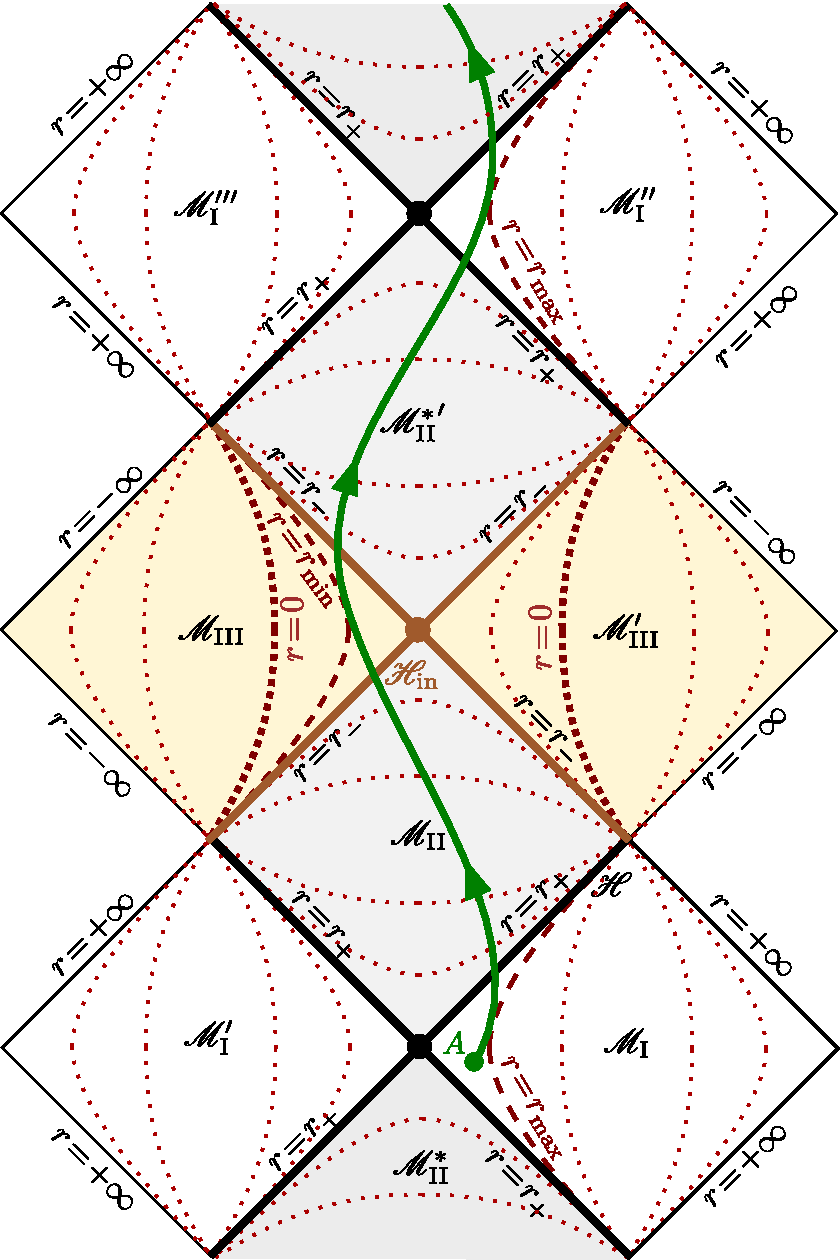
\includegraphics[width=0.6\textwidth]{gik_zero_ener_traj.pdf}}
\caption[]{\label{f:gik:zero_ener_traj} \footnotesize
Trajectory in the extended Kerr spacetime of a null geodesic
with $E=0$, $Q>0$ and $L<0$, emitted from a point $A$ in the outer ergoregion.
}
\end{figure}

The $\theta$-motion of $\Li$ is constrained by $\Theta(\th) \geq 0$ [Eq.~(\ref{e:gek:Theta_non_neg})],
which, given expression~(\ref{e:gik:Theta_E_zero}) for $\Theta$, is
equivalent to
\be
    \th_{\rm m} \leq \th \leq \pi - \th_{\rm m} \quad\mbox{with}\quad
    \th_{\rm m} := \arctan (-\bar{L}) .
\ee
\begin{remark}
The general formula for $\th_{\rm m}$ in the case
$a^2(E^2 - \mu^2) = 0$, Eq.~(\ref{e:gek:th0_a2E2mu2_zero}), which holds here since $\mu=0$ and $E=0$,
yields $\th_{\rm m} = \arccos\sqrt{1/(1+ \bar{L}^2)} = \arctan | \bar{L} |$.
Hence we recover the above formula.
\end{remark}
For $L = 0$, one has $\th_{\rm m} = 0$, so that $\th$ takes all values in the
range $[0,\pi]$, which means that $\Li$
crosses repeatedly the rotation axis. For $L< 0$, one has $0 < \th_{\rm m} < \pi/2$ and
$\Li$ oscillates symmetrically about the equatorial plane,
having two $\th$-turning points, at $\th_{\rm m} $ and $\pi-\th_{\rm m}$. Of course, we
recover the general results for $Q>0$ of Sec.~\ref{s:gek:th_motion}.

We can obtain $r$ as a function of $\th$ along $\Li$ by evaluating the integrals
in the identity (\ref{e:gek:integr_Mino}):
\[
    \dashint_{r_0}^r \frac{\eps_r \, \D \bar{r}}{\sqrt{R(\bar{r})}}
   = \dashint_{\th_0}^\th \frac{\eps_\th \, \D \bar{\th}}{\sqrt{\Theta(\bar{\th})}}
\]
Using (\ref{e:gik:R_E_zero_Lb}) and (\ref{e:gik:Theta_E_zero}), we get on
any portion of $\Li$ where $\eps_r$ and $\eps_\th$ are constant,
\[
    \eps_r \int_{r_0}^r
    \frac{\D \bar{r}}{\sqrt{- (1 + \bar{L}^2) \bar{r}^2 + 2m (1 + \bar{L}^2) \bar{r} - a^2}}
    = \eps_\th \int_{\th_0}^\th \frac{\D \bar{\th}}{\sqrt{1 - \bar{L}^2/\tan^2\bar{\th}}} .
\]
The changes of variables
\[
    x = \frac{r/m - 1}{\sqrt{1 - \frac{a^2}{m^2(1 + \bar{L}^2)}}}
    \qand
    \mu = \cos\th
\]
lead to
\[
   \frac{\eps_r}{\sqrt{1 + \bar{L}^2}} \int_{x_0}^x \frac{\D\bar{x}}{\sqrt{1 - \bar{x}^2}}
   = - \eps_\th \int_{\cos\th_0}^{\cos\th} \frac{\D\mu}{\sqrt{1 - (1 + \bar{L}^2)\mu^2}} .
\]
The integration is then immediate:
$\arcsin x = - \eps_r \eps_\th \arcsin(\sqrt{1 + \bar{L}^2} \cos\th) + K$,
where $K$ is a constant, from which we get
\be \label{e:gik:E_zero_r_theta}
   \encadre{ r = m + m\sqrt{1 - \frac{a^2}{m^2(1 + \bar{L}^2)}} \; \sin \left[
        K - \eps_r \eps_\th \arcsin\left(\sqrt{1 + \bar{L}^2} \cos\th\right) \right] }.
\ee
Since $\sqrt{1 + \bar{L}^2} \cos\th_{\rm m} = 1$, we see that the constant
$K$ is related to the value of $r$ at $\th = \th_{\rm m}$ by
\be \label{e:gik:E_zero_K}
    K =  \arcsin \left( \frac{r(\th_{\rm m})/m - 1}{\sqrt{1 - \frac{a^2}{m^2(1 + \bar{L}^2)}}} \right)
    + \eps_r \eps_\th \frac{\pi}{2} .
\ee
Note that $K$ is not a constant all along $\Li$, but only on portions where
$\eps_r$ and $\eps_\th$ are constant.
Expression~\ref{e:gik:E_zero_r_theta} gives the trace of the zero-energy
null geodesic $\Li$ in a meridional plane. It depends on $Q$ and $L$ only
through the ratio $\bar{L} := L / \sqrt{Q}$. It depends as well on the value of
$r$ at $\th_{\rm m}$ via $K$, as it appears in Eq.~(\ref{e:gik:E_zero_K}).
An example is shown in Fig.~\ref{f:gik:zero_ener_merid} for $a/m = 0.9$, $L / \sqrt{Q} = -1$
and $r(\th_{\rm m}) = 1.5\, m$. It has $\th_{\rm m} = \pi/4$,
$r_{\rm min} \simeq 0.229\, m$ and $r_{\rm max} \simeq 1.771\, m$,
while for $a/m = 0.9$, one has $r_- \simeq 0.564\, m$ and $r_+ \simeq 1.436\, m$.
For concreteness, the arrows indicate some direction of motion, but depending upon some
initial conditions, the opposite direction is possible.
In particular, one may consider that the geodesic is the same as that shown
in Fig.~\ref{f:gik:zero_ener_traj}, being emitted outward in the outer ergoregion
from a point $A$ in the equatorial plane ($\th=\pi/2$).

\begin{figure}
\centerline{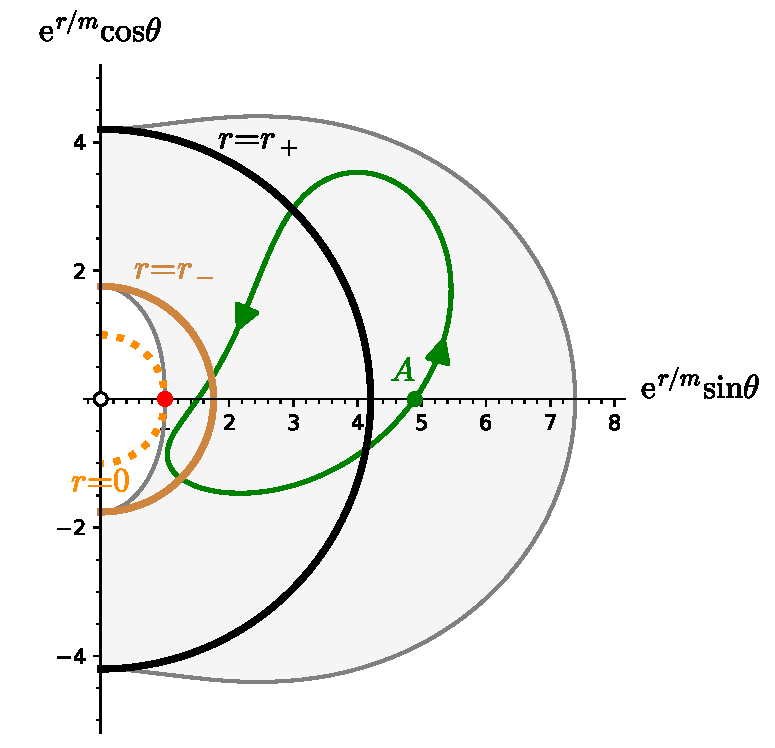
\includegraphics[width=0.6\textwidth]{gik_zero_ener_merid.pdf}}
\caption[]{\label{f:gik:zero_ener_merid} \footnotesize
Trajectory in the meridional plane, as given by Eq.~(\ref{e:gik:E_zero_r_theta}), of a null geodesic (green curve)
with $E=0$, $Q>0$, $L = - \sqrt{Q}$ and $r(\th_{\rm m}) = 1.5 \, m$
in the Kerr spacetime with $a/m = 0.9$.
The meridional plane is described in terms of
O'Neill exponential coordinates\index{O'Neill!coordinates} $x = \mathrm{e}^{r/m}\sin\th$ and $z = \mathrm{e}^{r/m}\cos\th$,
as in Figs.~\ref{f:ker:ergo_a90} -- \ref{f:ker:ergo_a99}.
The ergoregion is shown in grey.
The black (resp. blight rown) half-circle at $r=r_+$ (resp. $r=r_-$)
is the trace of the outer (resp. inner) Killing horizon.
The dotted orange half-circle marks the locus of $r=0$, with the
red dot indicating the curvature singularity at $r=0$ and $\th=\pi/2$.
The area $r> r_+$
corresponds to the regions $\M_{\rm I}$ and $\M_{\rm I}''$ in Fig.~\ref{f:gik:zero_ener_traj},
the area  $r_- < r < r_+$
corresponds to the regions $\M_{\rm II}$ and ${\M_{\rm II}^*}'$  in Fig.~\ref{f:gik:zero_ener_traj} and the area $r < r_-$
corresponds to the region $\M_{\rm III}$ in Fig.~\ref{f:gik:zero_ener_traj}.
\textsl{[Figure generated by the notebook \ref{s:sam:Kerr_null_geod_zero_ener}]}
}
\end{figure}

\subsubsection{Case $Q=0$}

If the zero-energy null geodesic $\Li$ has a vanishing Carter constant $Q$, Eq.~(\ref{e:gik:Theta_E_zero}) reduces to $\Theta(\th) = -L^2 / \tan^2\th$,
so that the constraint $\Theta(\th) \geq 0$ [Eq.~(\ref{e:gek:Theta_non_neg})]
implies $L=0$ or $\th = \pi/2$ .

In the first case, the four constants of motion $\mu$, $E$, $L$ and $Q$ are
zero. By virtue of the result (\ref{e:gek:all_const_zero}), $\Li$
is nothing but a null geodesic generator of the event horizon $\Hor$ or of the
inner horizon $\Hor_{\rm in}$.

In the second case ($\th=\pi/2$), $\Li$ is confined to the equatorial plane.
If $L=0$, we are back to the first case: $\Li$ is null geodesic generator of $\Hor$ or
$\Hor_{\rm in}$ lying in the equatorial plane.
If $L\neq 0$, the radial motion of $\Li$ is governed by Eq.~(\ref{e:gik:eom_r_E_zero}) with the
expression (\ref{e:gik:R_E_zero}) of $R(r)$ reduced to
\be
    R(r) = L^2 r (2m - r) .
\ee
The constraint $R(r) \geq 0$ [Eq.~(\ref{e:gek:R_non_neg})] implies then
that the motion is within the range $0 \leq r \leq 2 m$, with $r=2m$
being a $r$-turning point, since it is a simple root of $R(r)$ (cf. Sec.~\ref{s:gek:turning_points}).
It corresponds to the outer edge of the ergoregion in the equatorial plane,
cf. Eq.~(\ref{e:ker:r_ergo_p_eq}). Hence we have necessarily $\Li\cap \M_{\rm I} \neq \varnothing$
and (\ref{e:gik:E_zero_L_neg_ergo}) applies: $L < 0$.
The inner boundary of the radial motion, $r=0$, is the ring singularity.
Accordingly, in the maximally extended Kerr spacetime, $\Li$ starts at the ring
singularity in a $\M_{\rm III}$-type region (cf. Fig.~\ref{f:gik:zero_ener_traj_q0}),
has $r$ increasing, enters
a $\M_{\rm II}^*$-type region (time reversed copy of $\M_{\rm II}$), emerges
in $\M_{\rm I}$ via the white hole horizon at $r=r_+$ and reaches a $r$-turning point at
$r=2m$, then $r$ decreases continuously until $\Li$ terminates at the ring
singularity of $\M_{\rm III}$, after having crossed the black hole horizon $\Hor$
and the inner horizon $\Hor_{\rm in}$.
This trajectory, depicted in
Fig.~\ref{f:gik:zero_ener_traj_q0}, is similar to that for $Q\neq 0$
shown in Fig.~\ref{f:gik:zero_ener_traj}, except that it is ``blocked''
by two ring singularities and cannot oscillate forever between distinct
$\M_{\rm I}$-type regions.

\begin{figure}
\centerline{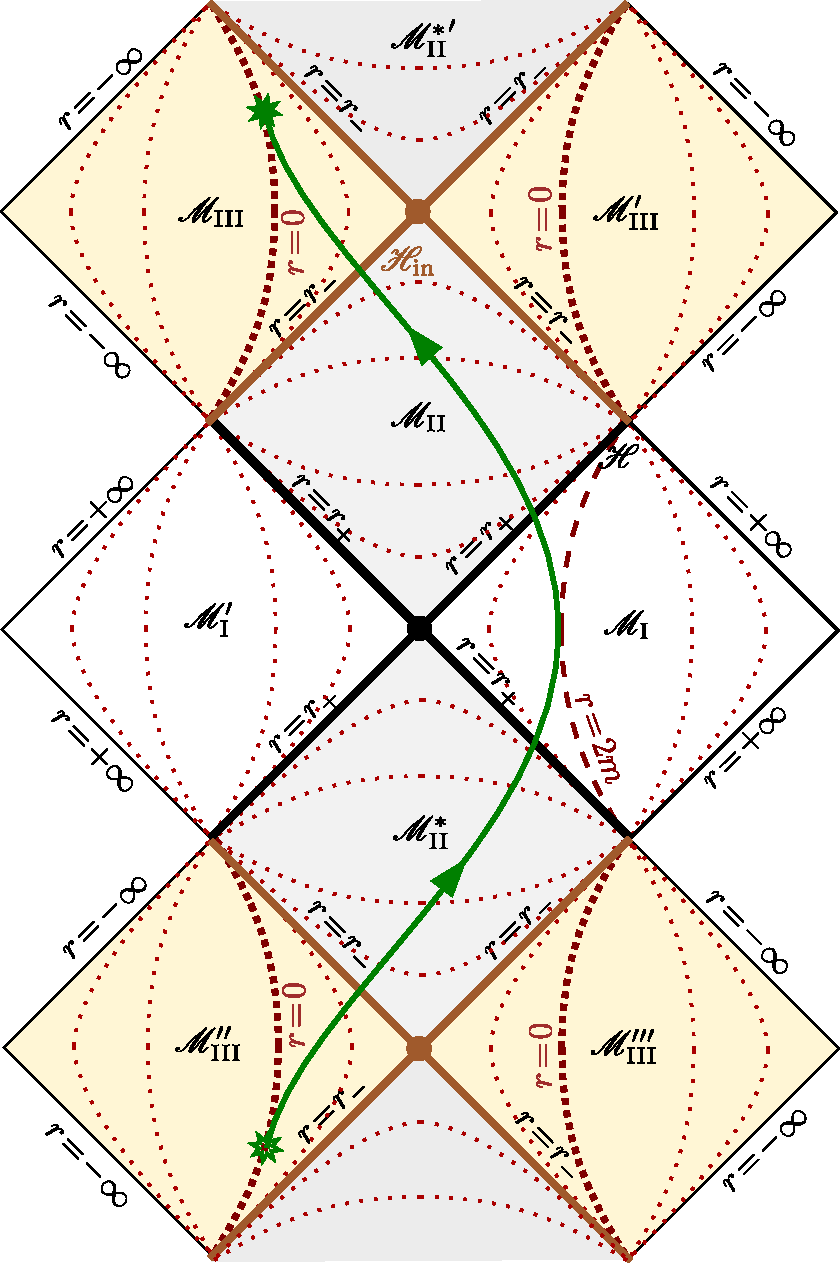
\includegraphics[width=0.6\textwidth]{gik_zero_ener_traj_q0.pdf}}
\caption[]{\label{f:gik:zero_ener_traj_q0} \footnotesize
Trajectory in the extended Kerr spacetime of a null geodesic
with $E=0$, $Q=0$ and $L<0$.
}
\end{figure}


\begin{remark}
For $Q\neq 0$ and $L\neq 0$, the limit $Q\to 0$ corresponds to
$\bar{L}^2 \to +\infty$ [cf. Eq.~(\ref{e:gik:def_L_bar})], so that
Eq.~(\ref{e:gik:E_zero_rmin_rmax}) yields
$r_{\rm min}\to 0$ and $r_{\rm max}\to 2m$.
We recover then the range $[0, 2m]$ for $r$ obtained here for $Q=0$.
\end{remark}


We conclude that
\begin{greybox}
Any null geodesic with $E=0$ and $Q=0$
is either a null generator of one of the two Killing horizons
$\Hor$ or $\Hor_{\rm in}$ (in which case, it has $L=0$) or it has
$L < 0$, lies in the equatorial plane,
emanates from a ring singularity, reaches the outer ergosphere ($r=2m$),
where it has a $r$-turning point, and terminates at a ring singularity.
\end{greybox}

Regarding the sign of $L$, we can combine the above result with that
obtained for $Q\neq 0$ [Eq.~(\ref{e:gik:E_zero_Qnz_L_neg})] to conclude:
\begin{greybox}
For $a\neq 0$, any null geodesic with $E=0$ has necessarily
\be
    \encadre{ L \leq 0 }_{{a\neq 0\atop E=0}}.
\ee
\end{greybox}

\begin{hist}
The zero-energy null geodesics in Kerr spacetime appear to have been first
studied by Zden\v{e}k Stuchl\'{\i}k\index{Stuchl\'{\i}k, Z.} in 1981, in the appendix
of the article~\cite{Stuch81}; some corrections and refinement of his results have been
performed by George Contopoulos\index{Contopoulos, G.} in 1984 \cite{Conto84},
who studied zero-energy timelike geodesics as well.
\end{hist}

\subsection{Equations of geodesic motion for $E\neq 0$} \label{s:gik:eom_Enonzero}

For any null geodesic $\Li$ with $E\neq 0$, we introduce the reduced constants of motion
\be \label{e:gik:def_ell_q}
    \encadre{\ell := \frac{L}{E}} \qand
    \encadre{q := \frac{Q}{E^2}} .
\ee
Note that, in geometrized units ($G=1$ and $c=1$), $\ell$ has the dimension of
a length and $q$ that of a squared length.

\begin{remark}
In the literature, $\ell$ is sometimes denoted by $\lambda$ (e.g. Refs.~\cite{Barde73,GrallL20b,DokucN20a})
or by $\xi$ (e.g. Ref.~\cite{Chand83}), while $q$ is sometimes denoted by
$\eta$ (e.g. Refs.~\cite{Barde73,Chand83,GrallL20b}). Moreover, in studies restricted
to $q\geq 0$, it may happen that the notation $q$ stands for the square root of the quantity $q$ defined by
(\ref{e:gik:def_ell_q}) (e.g. Refs.~\cite{DexteA09,GrallLS18,DokucN20a}).
\end{remark}

\begin{remark} \label{r:gik:ell_q_intrinsic}
Contrary to $L$ and $Q$,
the quantities $\ell$ and $q$ are independent from the affine parametrization of the geodesic $\Li$.
Indeed, if instead of the affine parameter $\lambda$ associated with the particle's 4-momentum $\w{p}$,
one considers the affine parameter $\lambda' = \alpha \lambda$, where $\alpha$ is a positive constant,
the tangent vector field becomes
$\w{p}' = \alpha^{-1} \w{p}$, so that the associated conserved
quantities are $E' = - \w{\xi}\cdot\w{p}' = \alpha^{-1} E$ [cf. Eq.~(\ref{e:gek:def_E})], $L' = \w{\eta}\cdot\w{p}' = \alpha^{-1} L$ [cf. Eq.~(\ref{e:gek:def_L})]
and $Q' = \w{\tilde K}(\w{p}',\w{p}') = \alpha^{-2} Q$ [cf. Eq. (\ref{e:gek:Q_tK_pp})],
so that $\ell' := L'/E' = \ell$ and $q' := Q'/{E'}^2 = q$.
\end{remark}

The nonnegative property of Carter constant $\mathscr{K}$ [Eq.~(\ref{e:ges:K_non_negative})],
along with the identity (\ref{e:gek:def_Q}) leads to the following constraint on
the parameters $\ell$ and $q$:
\be \label{e:gik:q_ell_a_constraint}
    \encadre{ q + (\ell - a)^2 \geq 0} .
\ee

\begin{example}[Principal null geodesic]
A principal null geodesic has $E\neq 0$ if, and only if, it does not belong to the outgoing
family generating the horizon $\Hor$ or $\Hor_{\rm in}$. This follows immediately from
Eqs.~(\ref{e:gek:ingoing_null_E_L}) and (\ref{e:gek:outgoing_null_E_L}).
One has then
$L = a E\sin^2\th_0$
[Eqs.~(\ref{e:gek:ingoing_null_E_L}) and (\ref{e:gek:outgoing_null_E_L})]
and $Q = - a^2 E^2 \cos^2\th_0$ [Eq.~(\ref{e:gek:Q_principal_null})], where
$\th_0$ is the constant value of $\th$ along the geodesic. We have thus
\be \label{e:gik:principal_null_l_q}
    \ell = a \sin^2\th_0 \qand q = - a^2 \cos^4\th_0 .
\ee
This yields
\be
    q + (\ell - a)^2  = 0 ,
\ee
so that (\ref{e:gik:q_ell_a_constraint}) is saturated for principal null
geodesics.
\end{example}

The equations of motion in term of the Mino parameter $\lambda'$,
Eqs.~(\ref{e:gek:eom_Mino}) specialized to $\mu=0$, can be rewritten as
\begin{subequations}
\label{e:gik:eom_Mino}
\begin{align}
& \encadre{ \frac{1}{E} \derd{t}{\lambda'} = \frac{1}{\Delta} \left[ (r^2 + a^2)^2 - 2 a m \ell r \right]   - a^2 \sin^2\th  } \label{e:gik:dtdl_Mino} \\
& \encadre{ \frac{1}{|E|} \derd{r}{\lambda'} = \eps_r \sqrt{ \mathcal{R}(r) } } \label{e:gik:drdl_Mino}\\
& \encadre{ \frac{1}{|E|} \derd{\th}{\lambda'} = \eps_\th \sqrt{\tilde\Theta(\th)} } \label{e:gik:dthdl_Mino}\\
& \encadre{ \frac{1}{E} \derd{\ph}{\lambda'}  = \frac{\ell}{\sin^2\th}
    + \frac{a}{\Delta}(2m r - a \ell) } , \label{e:gik:dphdl_Mino}
\end{align}
\end{subequations}
with
\be
    \mathcal{R}(r) := \frac{R(r)}{E^2}
    \qand
    \tilde\Theta(\th) := \frac{\Theta(\th)}{E^2} .
\ee
From the general expressions (\ref{e:gek:def_R_Q}), (\ref{e:gek:R_r_powers}) and (\ref{e:gek:Theta_Q}) specialized to $\mu=0$, we get
\begin{subequations}
\label{e:gik:mcR}
\begin{align}
    &\encadre{\mathcal{R}(r) = (r^2 + a^2 - a \ell)^2 - \Delta \left[ q + (\ell -a)^2 \right] }
      \label{e:gik:mcR_Delta}\\
    &\encadre{\mathcal{R}(r) =  r^4 + (a^2 - \ell^2 - q) r^2 + 2m\left[ q + (\ell -a)^2 \right] r
    - a^2 q } \label{e:gik:mcR_powers}
\end{align}
\end{subequations}
and
\be \label{e:gik:tTheta}
    \encadre{ \tilde\Theta(\th) = q + \cos^2\th \left( a^2
    - \frac{\ell^2}{\sin^2\th} \right) } .
\ee

It suffices to use the parameter $\lambda'' := |E| \lambda'$ to make $E$
disappear from the system~(\ref{e:gik:eom_Mino}). We therefore conclude that
\begin{greybox}
In Kerr spacetime, a null geodesic with $E\neq 0$  is entirely determined
by the two constants $(\ell,q)$, by the sign of $E$ and by the values of the two
signs $\eps_r=\pm 1$ and $\eps_\th=\pm 1$ at a given point.
\end{greybox}

\begin{example}[Principal null geodesic]
Given the values (\ref{e:gik:principal_null_l_q}) of $\ell$ and $q$
for a principal null geodesic, Eq.~(\ref{e:gik:mcR_powers}) reduces to
a simple expression for the quartic polynomial $\mathcal{R}$:
\be \label{e:gik:mR_PNG}
    \mathcal{R}(r) = \left( r^2 + a^2 \cos^2 \th_0 \right)^2 .
\ee
We note that $\mathcal{R}(r) = \rho^4$, which makes sense because $\th = \th_0$
is constant along such a geodesic. For any principal null geodesic lying
in the equatorial plane, the polynomial simplifies even further:
\be
    \mathcal{R}(r) = r^4 \qquad \left(\th_0 = \frac{\pi}{2} \right) .
\ee
\end{example}

\begin{figure}
\centerline{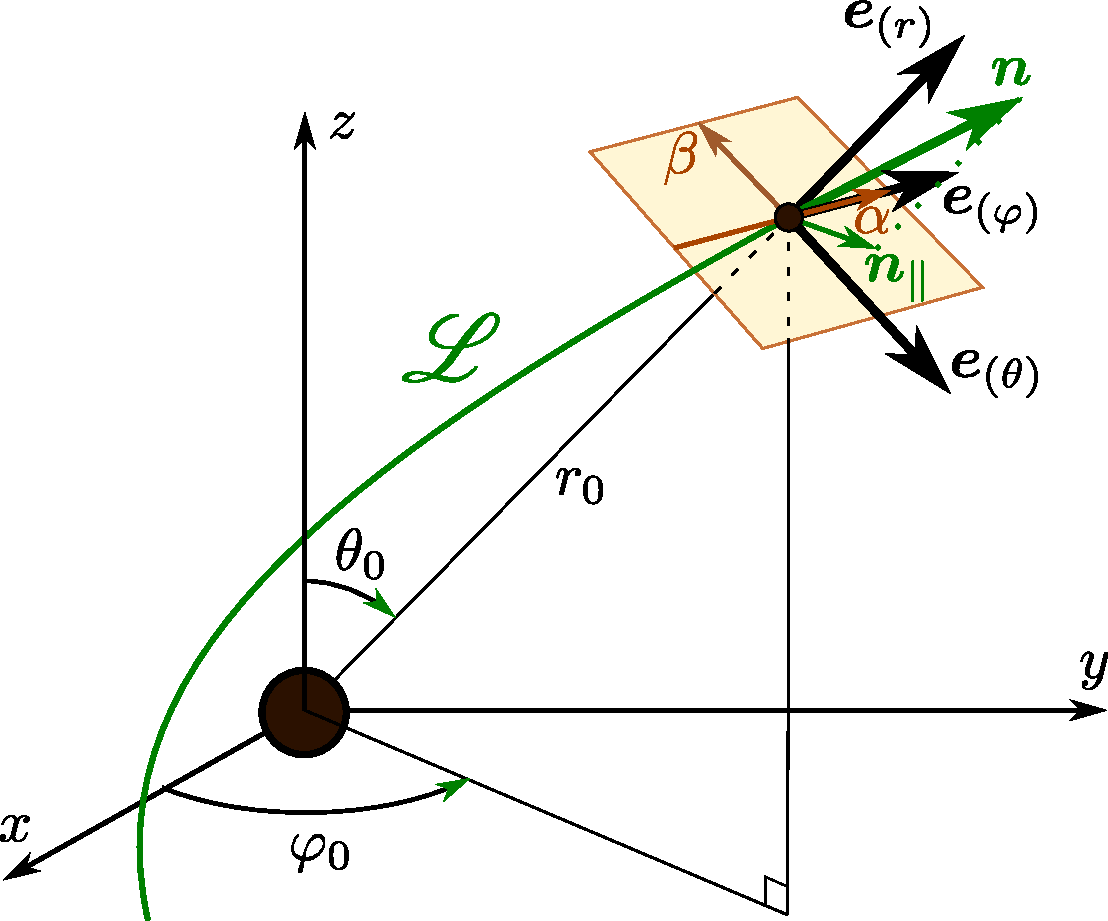
\includegraphics[width=0.6\textwidth]{gik_obs_screen.pdf}}
\caption[]{\label{f:gik:obs_screen} \footnotesize
Impact of a null geodesic $\Li$ onto the screen of a remote observer. $(x,y,z)$ are the Cartesian Boyer-Lindquist coordinates
defined by Eq.~(\ref{e:gek:Cartesian_BL}).
}
\end{figure}

\subsection{Position on a remote observer's screen} \label{s:gik:remote_screen}

The constants $(\ell,q)$ are closely related to the impact coordinates $(\alpha,\beta)$
on the screen of an asymptotic inertial observer (cf. Sec.~\ref{s:ker:asymp_inertial_obs})
in case the null geodesic $\Li$ reaches the asymptotic region $r\to +\infty$.
Indeed, let us consider an asymptotic inertial observer $\Obs$ located at (fixed) Boyer-Lindquist
coordinates $(r_{\Obs}, \th_{\Obs}, \ph_{\Obs})$, with $r_{\Obs} \gg m$ (cf. Fig.~\ref{f:gik:obs_screen}).
In order to reach $\Obs$, the geodesic $\Li$ must be such that the constraints
constraints $\mathcal{R}(r_{\Obs}) \geq 0$
[Eq.~(\ref{e:mcR_non_neg})]
and $\tilde\Theta(\th_{\Obs}) \geq 0$ [Eq.~(\ref{e:gek:Theta_non_neg})]
are fulfilled.
The first one is always satisfied due to the
assumption that $\Obs$ is an asymptotic observer, since
$\mathcal{R}(r) \sim r^4$ for $r\to +\infty$ [cf. Eq.~(\ref{e:gik:mcR_powers})].
In view of expression~(\ref{e:gik:tTheta}) for $\tilde\Theta$, the second
constraint is equivalent to
\be \label{e:gik:constraint_theta_obs}
    \left( q + a^2 \cos^2\th_{\Obs} \right) \sin^2\th_{\Obs}
         - \ell^2 \cos^2\th_{\Obs} \geq 0 .
\ee
If $\sin\th_{\Obs}$ is small,
this constraint limits significantly the amplitude of $\ell$.

\subsubsection{Observer not located on the rotation axis}

Here we treat the generic case of an observer $\Obs$ that is not located on the rotation axis,
i.e. we assume $\th_{\Obs}\not\in\{0,\pi\}$.
The orthonormal frame of $\Obs$ is $\w{e}_{(0)} =\w{\xi}$, $\w{e}_{(r)} = \wpar_r$,
$\w{e}_{(\th)} = r_{\Obs}^{-1} \wpar_\th$ and $\w{e}_{(\ph)} = (r_{\Obs}\sin\th_{\Obs})^{-1} \wpar_\ph$
[Eq.~(\ref{e:ker:def_ZAMO_frame}) with $r = r_{\Obs}\to +\infty$].
Let us assume that the observer set up a screen (via a telescope) centered on the direction to the
black hole, i.e. such that $\w{e}_{(r)}$ is the normal to the screen. The 4-momentum of the photon
having $\Li$ as worldline at the location of $\Obs$ writes
\[
    \w{p} = p^t \, \w{\xi} + p^r \, \w{e}_{(r)} + p^\th r_{\Obs} \, \w{e}_{(\th)}
    + p^\ph r_{\Obs} \sin\th_{\Obs} \, \w{e}_{(\ph)} =  E (\w{\xi} + \w{n}) ,
\]
where the second equality follows from the orthogonal decomposition (\ref{e:fra:p_E_V}) with respect to
$\Obs$, $\w{\xi}$ being the 4-velocity of $\Obs$ and the unit spacelike vector $\w{n}$ being the photon's velocity\footnote{$\w{n}$ is denoted by $\w{V}$ in Eq.~(\ref{e:fra:p_E_V}).} relative to $\Obs$; it
obeys $\w{\xi}\cdot\w{n} = 0$ and $\w{n}\cdot\w{n} = 1$ [Eq.~(\ref{e:fra:photon_V_one})].
That the conserved energy $E$ appears in the above equation is a direct consequence of its
definition as $E := - \w{\xi}\cdot \w{p}$ [Eq.~(\ref{e:gek:def_E})] with $\w{\xi}\cdot\w{\xi} = -1$
for $r_{\Obs}\to +\infty$. The above identity implies
$p^t = E$ and
\[
    \w{n} = \frac{p^r}{E} \, \w{e}_{(r)} + \frac{p^\th}{E} r_{\Obs} \, \w{e}_{(\th)}
    + \frac{p^\ph}{E} r_{\Obs} \sin\th_{\Obs} \, \w{e}_{(\ph)} .
\]
With respect to $\Obs$, the incoming direction of the photon is given by
the vector $-\w{n}$ and the trace on the screen is indicated by the component of that
vector that is tangent to the screen, namely
\be \label{e:gik:m_screen_p}
    \w{m} = - \w{n}_{\parallel} = - \frac{p^\th}{E} r_{\Obs} \, \w{e}_{(\th)}
    -  \frac{p^\ph}{E} r_{\Obs} \sin\th_{\Obs} \, \w{e}_{(\ph)}
\ee
since the screen plane is spanned by $\w{e}_{(\th)}$ and $\w{e}_{(\ph)}$
(cf. Fig.~\ref{f:gik:obs_screen}). Let us choose the screen dimensionless
Cartesian coordinates $(\alpha,\beta)$ so that the black hole's rotation axis
appears as the $\beta$-axis (cf. Fig.~\ref{f:gik:obs_screen}), then
\be \label{e:gik:m_screen_ab}
    \w{m} = \alpha \w{e}_{(\alpha)} + \beta \w{e}_{(\beta)}, \quad\mbox{with}\quad
    \w{e}_{(\alpha)} = \w{e}_{(\ph)} \quad\mbox{and}\quad
    \w{e}_{(\beta)} = - \w{e}_{(\th)} .
\ee
By comparing with (\ref{e:gik:m_screen_p}), we get
\[
    \alpha = -  \frac{p^\ph}{E} r_{\Obs} \sin\th_{\Obs}
    \qand
    \beta = \frac{p^\th}{E} r_{\Obs} .
\]
Now, for $r_{\Obs}\to +\infty$,
\[
   \frac{p^\th}{E} = \frac{1}{E} \derd{\th}{\lambda} = \frac{1}{E r_{\Obs}^2}  \derd{\th}{\lambda'} =
    \frac{\eps_\th}{r_{\Obs}^2} \sqrt{\tilde\Theta(\th_{\Obs})}
\]
\[
 \frac{p^\ph}{E} = \frac{1}{E} \derd{\ph}{\lambda} = \frac{1}{E r_{\Obs}^2}  \derd{\ph}{\lambda'}
 = \frac{\ell}{r_{\Obs}^2 \sin^2\th_{\Obs}} ,
\]
where we have used Eqs.~(\ref{e:gik:dthdl_Mino}) and (\ref{e:gik:dphdl_Mino}), with the
term involving $a/\Delta$ neglected since $\Delta \sim r^2$ for $r\to +\infty$.
By inserting these formula into the above expressions of $\alpha$ and $\beta$,
and using Eq.~(\ref{e:gik:tTheta}) for $\tilde\Theta(\th_{\Obs})$,
we get the sought relation between the constants of motion $(\ell, q)$ and
the screen coordinates:
\begin{subequations}
\label{e:gik:screen_alpha_beta}
\begin{align}
& \encadre{ \alpha = - \frac{\ell}{r_{\Obs}\sin\th_{\Obs}} } \\
& \encadre{ \beta = \frac{\eps_\th}{r_{\Obs}} \sqrt{ q + \cos^2\th_{\Obs} \left( a^2
    - \frac{\ell^2}{\sin^2\th_{\Obs}} \right) } } .
\end{align}
\end{subequations}

We have defined $(\alpha,\beta)$ as dimensionless Cartesian coordinates on
the screen, cf. Eq.~(\ref{e:gik:m_screen_ab}), where $\w{m}$ is
dimensionless and $(\w{e}_{(\alpha)}, \w{e}_{(\beta)})$
is the screen's orthonormal basis. In practice, their values are tiny,
being exactly zero at the limit $r_{\Obs}\to +\infty$. $(\alpha,\beta)$ can thus be interpreted as
\emph{angular} coordinates, measuring the departure from the direction
of the black hole ``center'' on the celestial sphere of observer $\Obs$.
We shall then call $(\alpha,\beta)$ the
\defin{screen angular coordinates}\index{screen!angular coordinates}\index{angular!screen -- coordinates}.

\begin{remark}
When studying null geodesics in Schwarzschild spacetime in Chap.~\ref{s:gis}, we
introduced the impact parameter $b$ as $b := |L|/E$ [Eq.~(\ref{e:ges:def_b})], hence
$b$ is related to $\ell$ by
\be
    b = |\ell| .
\ee
Moreover, thanks to spherical symmetry, we could reduce the study to the case
where both the observer
and the geodesic lie in the equatorial plane, which imply $\th_{\Obs} = \pi/2$
and $q=0$. Equations~(\ref{e:gik:screen_alpha_beta}) yield then
\be
    |\alpha| = \frac{b}{r_{\Obs}} = \hat{b} \qand \beta = 0 ,
\ee
where $\hat{b}$ is the angle introduced by formula (\ref{e:gis:hat_b}).
\end{remark}

\begin{remark}
The angular impact parameters $(\alpha, \beta)$ depend on the geodesic $\Li$ as a curve
in spacetime and not on any affine parametrization of $\Li$. Their direct
connection with $(\ell, q)$ expressed by (\ref{e:gik:screen_alpha_beta}) is thus in
perfect agreement with the invariance of $(\ell, q)$ in any affine reparametrization
of $\Li$, as noticed in Remark~\ref{r:gik:ell_q_intrinsic} p.~\pageref{r:gik:ell_q_intrinsic}.
\end{remark}

We deduce from Eqs.~(\ref{e:gik:screen_alpha_beta}) a
simple relation between the squared angular distance to the screen center, $\alpha^2 + \beta^2$,
and the constants of motion $(\ell, q)$ of the incoming geodesic:
\be \label{e:gik:alpha2_beta2}
    \alpha^2 + \beta^2 = \frac{1}{r_{\Obs}^2} \left(
    \ell^2 + q + a^2 \cos^2\th_{\Obs} \right) .
\ee
%The asymptotic formula (\ref{e:gek:Q_Ltot2_L2}) relates $\ell^2 + q = E^{-2} (L^2 + Q)$
%to the square of the total angular momentum $\w{L}_{\rm tot}$ of the incoming
%photon as measured by observer $\Obs$. Using it, we can turn (\ref{e:gik:alpha2_beta2})
%into
%\be
    %r_{\Obs}^2 (\alpha^2 + \beta^2) = \frac{\w{L}_{\rm tot}\cdot\w{L}_{\rm tot}}{E^2}
        %+ 2 a \frac{L}{E} - a^2 \sin^2\th_{\Obs} .
%\ee

\subsubsection{Observer on the rotation axis}

If the asymptotic inertial observer $\Obs$ is located on the rotation axis,
i.e. if $\th_{\Obs}=0$ or $\th_{\Obs} = \pi$,
the only value of $\ell$ compatible with
the constraint (\ref{e:gik:constraint_theta_obs}) is
\be \label{e:gik:obs_axis_ell_zero}
     \ell = 0 \qquad (\th_{\Obs} = 0\ \mbox{or}\  \th_{\Obs} = \pi).
\ee
Given that $\ell = L/E$, we
recover one of the properties listed in Sec.~\ref{s:gek:th_motion}:
a geodesic cannot encounter the rotation axis unless it has $L = 0$.

Moreover, on the rotation axis,
the vectors $\w{e}_{(\th)}$
and $\w{e}_{(\ph)}$ are not defined, due to the singularity of spherical
coordinates there. Consequently, the screen coordinates $(\alpha,\beta)$
cannot be defined by (\ref{e:gik:m_screen_ab}). In particular, the rotation axis appears as
single point on the screen, which forbids to use it to define the $\beta$-axis.
One has then to pick an arbitrary orthonormal frame
$(\w{e}_{(\alpha)}, \w{e}_{(\beta)})$ in the screen plane to define
$(\alpha,\beta)$. Formulas (\ref{e:gik:shadow_param_eq}) do no longer
hold, but formula (\ref{e:gik:alpha2_beta2}) is still valid,
since the distance from the screen's center is a quantity independent from
the orientation of the frame $(\w{e}_{(\alpha)}, \w{e}_{(\beta)})$. Another
way to see that (\ref{e:gik:alpha2_beta2}) is still valid is to notice that
it admits a well-defined limit for $\th_{\Obs}\to 0$ or $\pi$. Taking into
account $\ell=0$, we obtain
\be \label{e:gik:alpha2_beta2_axis}
    \alpha^2 + \beta^2 = \frac{1}{r_{\Obs}^2} \left( q + a^2\right)
    \qquad (\th_{\Obs} = 0\ \mbox{or}\  \th_{\Obs} = \pi).
\ee


\subsection{Latitudinal motion} \label{s:gik:th_motion}

Specializing the general results of Sec.~\ref{s:gek:th_motion} to $\mu=0$, we
get
\begin{greybox}
\begin{itemize}
\item A null geodesic $\Li$ of Kerr spacetime cannot encounter the rotation axis unless it has $\ell=0$.
\item If $|\ell|\geq a$,
the reduced Carter constant $q$ is necessarily nonnegative:
\be \label{e:gik:q_nonnegative}
    q \geq 0 .
\ee
\item The reduced Carter constant $q$ can take negative values only if $|\ell|<a$
(which implies  $a\neq 0$); its range is then
limited from below:
\be \label{e:gik:q_min}
    q \geq q_{\rm min} = - \left( a - |\ell| \right) ^2.
\ee
If $q<0$, $\Li$ is called a \defin{vortical null geodesic}\index{vortical geodesic}; it
never encounters the equatorial plane.
\item If $q>0$ and $\ell\not=0$, $\Li$ oscillates symmetrically about the equatorial plane,
between two $\th$-turning points, at $\th=\th_{\rm m}$ and $\th=\pi-\th_{\rm m}$,
where $\th_{\rm m}\in(0,\pi/2)$
is given by Eqs.~(\ref{e:gek:th0_a2E2mu2_zero}) and (\ref{e:gek:th0_E_gt_mu}):
\begin{align}
    &  \th_{\rm m} = \arccos\sqrt{\frac{q}{\ell^2 + q}} \quad\mbox{for}\quad a=0\\
    &  \th_{\rm m} =  \arccos  \sqrt{   \frac{1}{2} \left[ 1 - \frac{\ell^2 + q}{a^2}
        + \sqrt{ \left(1 - \frac{\ell^2 + q}{a^2}\right) ^2
        + \frac{4q}{a^2} } \right]  }  \quad\mbox{for}\quad a\neq 0 . \label{e:gik:th0}
\end{align}
If $q>0$ and $\ell=0$, $\Li$
crosses repeatedly the rotation axis, with $\th$ taking all values in the
range $[0,\pi]$.
\item If $q=0$, $\Li$ is stably confined to the equatorial plane
for $|\ell| > a$ or $|\ell| = a\neq 0$;
for $|\ell| < a$, $\Li$ either lies unstably in the equatorial
plane or approaches it asymptotically from one side, while for $\ell=0$ and $a=0$,
$\Li$ lies at a constant value $\th=\th_0\in[0,\pi]$.
\item If $q_{\rm min} < q < 0$, $\Li$ never encounters the equatorial plane,
having a $\th$-motion entirely confined either to the Northern hemisphere
($0<\th<\pi/2$) or to
the Southern one ($\pi/2<\th<\pi$); if $\ell\neq 0$, $\Li$ oscillates between
two $\th$-turning points, at $\th=\th_{\rm m}$ and $\th=\th_{\rm v}$ (Northern hemisphere)
or at $\th=\pi-\th_{\rm v}$ and $\th=\pi-\th_{\rm m}$ (Southern hemisphere), where
$\th_{\rm m}$ is given by Eq.~(\ref{e:gik:th0}) above and $\th_{\rm v}$ is given
by  Eq.~(\ref{e:gek:th1}):
\be \label{e:gik:th1_general}
   \th_{\rm v} =  \arccos  \sqrt{  \frac{1}{2} \left[ 1 - \frac{\ell^2 + q}{a^2}
        - \sqrt{ \left(1 - \frac{\ell^2 + q}{a^2}\right) ^2
        + \frac{4q}{a^2}} \right]  }  ;
\ee
if $\ell=0$,
$\Li$ oscillates about the rotation axis, with a $\th$-turning point at
$\th=\th_{\rm v}$ or $\th = \pi - \th_{\rm v}$, where $\th_{\rm v}$
is given by Eq.~(\ref{e:gek:th0_L_zero}), or equivalently by the $\ell\to 0$
limit of Eq.~(\ref{e:gik:th1_general}):
\be \label{e:gik:thv_ell_zero}
    \th_{\rm v} = \arccos \left( \frac{\sqrt{-q}}{a} \right) \qquad (\ell=0) .
\ee
\item If $q = q_{\rm min}$, $\Li$ lies stably at a constant value
$\th=\th_*$ or $\th = \pi - \th_*$, with $\th_*\in [0, \pi/2)$%]$
\ given by
\be \label{e:gik:th_s_ell_over_a}
     \th_* := \arcsin\sqrt{\frac{|\ell|}{a}} .
\ee
\end{itemize}
\end{greybox}

\begin{remark}
For $\ell < 0$, the constraint (\ref{e:gik:q_min}) is tighter than
(\ref{e:gik:q_ell_a_constraint}).
\end{remark}

\begin{example}[Principal null geodesic]
A principal null geodesic moves at a constant angle
$\th=\th_0$ and has
$\ell = a\sin^2\th_0$ [Eq.~(\ref{e:gik:principal_null_l_q})].
For $\th_0\neq \pi/2$, we have $|\ell| < a$ and
Eq.~(\ref{e:gik:q_min}) yields $q_{\rm min} = - a^2 \cos^4\th_0$.
Comparing with the value of $q$ given by Eq.~(\ref{e:gik:principal_null_l_q}),
we note that
\be
     q = q_{\rm min} ,
\ee
which agrees with the last case listed above, i.e. motion at constant
$\th$, with $\th_0 = \th_*$ or $\th_0 = \pi - \th_*$ according
to Eq.~(\ref{e:gik:th_s_ell_over_a}), since $\sqrt{|\ell|/a} = \sin\th_0$.
\end{example}

\subsection{Radial motion} \label{s:gik:radial_motion}

As for any geodesic, the radial motion of a null geodesic $\Li$ is ruled by
$R(r)\geq 0$ [Eq.~(\ref{e:gek:R_non_neg})], which, in terms of $\mathcal{R}(r)$
[Eq.~(\ref{e:gik:mcR})],
writes
\be \label{e:mcR_non_neg}
    \encadre{\mathcal{R}(r) \geq 0 }.
\ee

\begin{example}[Principal null geodesic]
Given the value (\ref{e:gik:mR_PNG}) of $\mathcal{R}(r)$ for
a principal null geodesic, we note that
$\mathcal{R}(r) > 0$ in all Kerr spacetime. This is
consistent with the fact that, for $E\neq 0$ and $\th_0\neq\pi/2$, ingoing principal null geodesics
travel from $r=+\infty$ to $r=-\infty$ (cf. the dashed green curve
in Fig.~\ref{f:ker:3blocks_in}) and outgoing principal null geodesics
travel from $r=-\infty$ to $r=+\infty$ (cf. the solid green curve
in Fig.~\ref{f:ker:3blocks_out}).
\end{example}

\begin{figure}
\begin{tabular}{c@{\hspace{-0.2ex}}c@{\hspace{-0.2ex}}c@{\hspace{-0.2ex}}c}
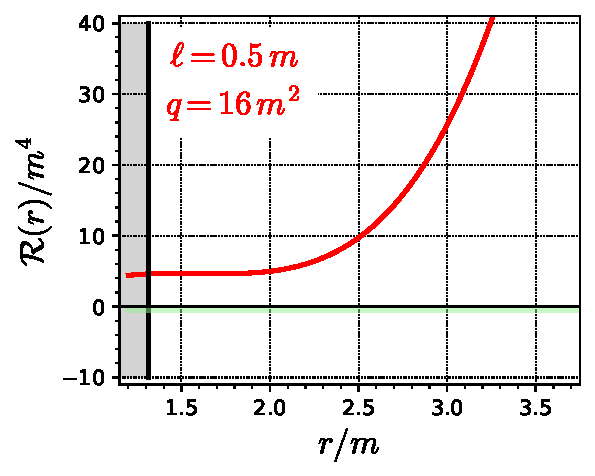
\includegraphics[height=0.15\textheight]{gik_R_in_M1_1.pdf}
& 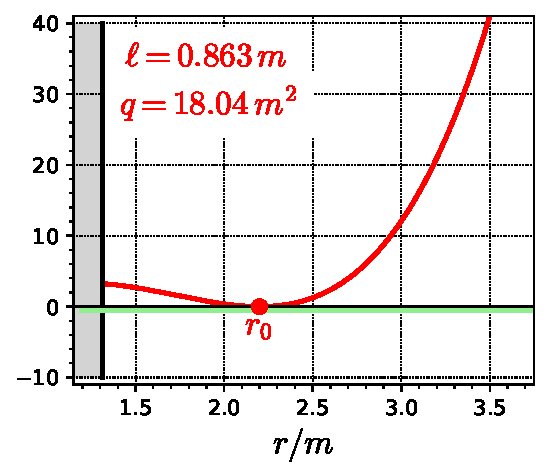
\includegraphics[height=0.15\textheight]{gik_R_in_M1_2.pdf}
&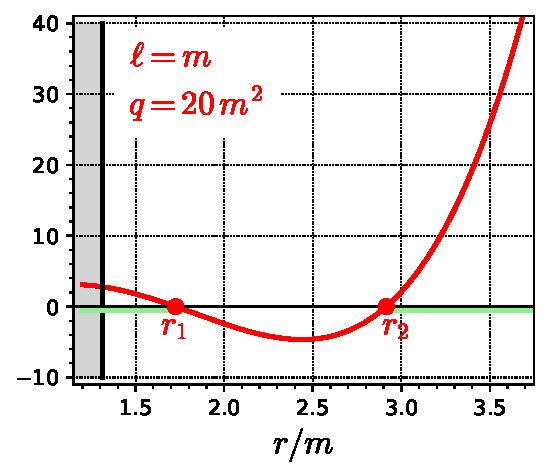
\includegraphics[height=0.15\textheight]{gik_R_in_M1_3.pdf}
&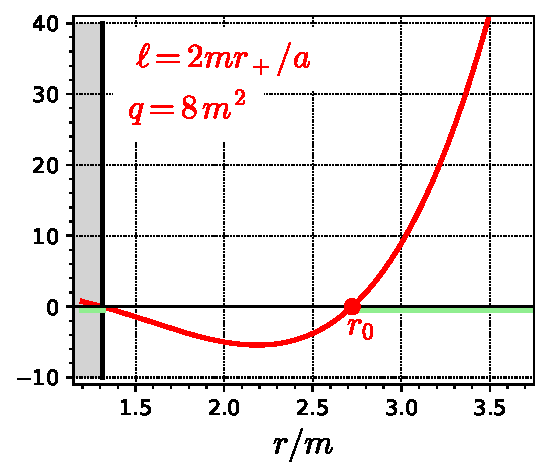
\includegraphics[height=0.15\textheight]{gik_R_in_M1_4.pdf}\\[-1.5ex]
(a) & (b) & (c)& (d)
\end{tabular}
\caption[]{\label{f:gik:R_in_M1} \footnotesize
Quartic polynomial $\mathcal{R}(r)$ in the region $\M_{\rm I}$ for
four values of $(\ell, q)$ and for $a=0.95\, m$.
The grey area marks the black hole region, with the vertical
black line at the event horizon, at $r=r_+ \simeq 1.312\, m$.
The green part of the $r$ axis corresponds to $\mathcal{R}(r) \geq 0$,
i.e. to regions where the geodesic motion is allowed.
\textsl{[Figure generated by the notebook \ref{s:sam:Kerr_null_geod_plots}]}
}
\end{figure}

Since $\mathcal{R}(r)$ is a polynomial of degree $4$ in $r$, its
behavior can be relatively complicated. However, it turns out that in the
black hole exterior, its behavior is quite simple, according to the
following lemma:
\begin{greybox}
\textbf{Lemma ($\mathcal{R}(r)$ in $\M_{\rm I}$)}\\[1ex]
In region $\M_{\rm I}$ of Kerr spacetime, i.e. for $r> r_+$, the
quartic polynomial $\mathcal{R}(r)$ associated to a given geodesic
[Eq.~(\ref{e:gik:mcR})] has one of the following behaviors, depending
on the value of $(\ell, q)$:
\begin{enumerate}
\item $\mathcal{R}(r)$ has no root in $(r_+,+\infty)$ and $\mathcal{R}(r) > 0$
there (Fig.~\ref{f:gik:R_in_M1}a);
\item $\mathcal{R}(r)$ has a double root in $(r_+,+\infty)$, at $r=r_0$ say, and
$\mathcal{R}(r) > 0$ iff $r\in(r_+, r_0)$ or $r\in(r_0, +\infty)$
(Fig.~\ref{f:gik:R_in_M1}b);
\item $\mathcal{R}(r)$ has two simple roots in $(r_+,+\infty)$, at $r=r_1$ and $r=r_2$ say, and
$\mathcal{R}(r) > 0$ iff $r\in(r_+, r_1)$ or $r\in(r_2, +\infty)$
(Fig.~\ref{f:gik:R_in_M1}c);
\item $\mathcal{R}(r)$ has a unique simple root in $(r_+,+\infty)$, at $r=r_0$ say; then
necessarily $\ell = 2 m r_+ /a$, $\mathcal{R}(r_+) = 0$ and
$\mathcal{R}(r) > 0$ iff $r\in(r_0, +\infty)$
(Fig.~\ref{f:gik:R_in_M1}d).
\end{enumerate}
\end{greybox}
\begin{proof}
First, we observe that $\mathcal{R}(r)$ is positive or zero at both
ends of $\M_{\rm I}$. This is clear
for the asymptotic flat end since, according to expression~(\ref{e:gik:mcR_powers}),
$\mathcal{R}(r) \sim r^4 > 0$ when $r\to +\infty$. At the inner end,
namely for $r \to r_+$,
we have $\Delta \to 0$ and expression~(\ref{e:gik:mcR_Delta}) yields the limit value
$\mathcal{R}(r_+) = (r_+^2 + a^2 - a \ell)^2 \geq 0$.
Now, as a polynomial of degree four, $\mathcal{R}(r)$ has at most four real roots.
Given the above boundary conditions, $\mathcal{R}(r)$ can have
a unique simple root in $(r_+,+\infty)$ only if $\mathcal{R}(r_+) = 0$ (cf. Fig.~\ref{f:gik:R_in_M1}d),
which occurs for a very specific value of $\ell$, namely $\ell = (r_+^2 + a^2)/a = 2 m r_+/a$.
This is case~4 above.
Similarly, the case of three roots in $(r_+,+\infty)$, either three simple roots or one double and one simple root,
is compatible with the boundary conditions only if $\mathcal{R}(r_+) = 0$, i.e.
if $r_+$ is a fourth root of $\mathcal{R}(r)$.
But then the four roots of $\mathcal{R}(r)$ would be positive (since $r_+ > 0$).
Now, since there is no $r^3$ term in the expression~(\ref{e:gik:mcR_powers}) of $\mathcal{R}(r)$,
the sum of the roots of $\mathcal{R}(r)$ is zero, which is impossible with all
the roots being positive. Hence there cannot be three roots in $(r_+,+\infty)$.
The same argument about the zero sum of the roots excludes as well the case
of four roots of $\mathcal{R}(r)$ in $(r_+,+\infty)$.
There remains then the cases of no root at all in  $(r_+,+\infty)$ (case 1 of the lemma) and that of two
roots (cases 2 and 3). These three cases are compatible
with the boundary conditions and the vanishing of the sum of the roots.
\end{proof}

\begin{remark}
Case~4 of the lemma can be seen as the limit $r_1\to r_+$ of case~3.
\end{remark}

\begin{remark}
In case~4, $\mathcal{R}(r_+) = 0$ occurs for $\Omega_H \ell = 1$, where $\Omega_H$ is the black hole
rotation velocity\index{black hole!rotation velocity}\index{rotation!velocity},
as given by Eq.~(\ref{e:ker:def_OmegaH}). Similarly, $\mathcal{R}(r_-) = 0$ for $\Omega_{\rm in} \ell = 1$,
where $\Omega_{\rm in}$ is the rotation velocity of the inner horizon, cf. Eq.~(\ref {e:ker:def_Omega_in}).
\end{remark}

\begin{remark} \label{r:gik:R_zero_M_III}
The region $\M_{\rm III}$ shares with $\M_{\rm I}$ that $\mathcal{R}(r)$ is
nonnegative at each of its ends: $\mathcal{R}(r) \sim r^4 > 0$ when $r\to -\infty$
and $\mathcal{R}(r_-) = (r_-^2 + a^2 - a \ell)^2 \geq 0$. However, the argument
used to limit the number of roots in $\M_{\rm I}$
cannot be applied to $\M_{\rm III}$ because the latter can accommodate for both positive and negative
values of $r$ and thus four roots of $\mathcal{R}(r)$ can be located in $\M_{\rm III}$.
\end{remark}


According to the definition given in Sec.~\ref{s:gek:turning_points},
a $r$-turning of a null geodesic $\Li$ is a point $p_0\in \Li$
such that $r_0 := r(p)$ is a simple root of $\mathcal{R}(r)$.
The above lemma leads then to:
\begin{greybox}
A null geodesic in Kerr spacetime has
\begin{itemize}
\item at most one $r$-turning point in region $\M_{\rm I}$;
\item no $r$-turning point in region $\M_{\rm II}$.
\end{itemize}
\end{greybox}
\begin{proof}
If a geodesic would have two turning points in $\M_{\rm I}$, this would mean
that there exist two simple roots in $\M_{\rm I}$ and that
$\mathcal{R}(r)$ is positive between them (so that the motion is possible
there). But this is excluded by the lemma.
In region $\M_{\rm II}$, we have $\Delta < 0$ and
Eqs.~(\ref{e:gik:mcR_Delta}) and (\ref{e:gik:q_ell_a_constraint}) show that
$\mathcal{R}(r)$ is the sum of two nonnegative terms. The only possibility
to have $\mathcal{R}(r)=0$ is then that each term vanishes separately:
$r^2 + a^2 - a\ell = 0$ and $q + (\ell -a)^2 = 0$, i.e.
\[
  r^2 = a (\ell - a) \qand q = - (\ell - a)^2 .
\]
The second equation implies $q\leq 0$. The case $q=0$ would lead to $\ell = a$ and $r^2 = 0$,
which is impossible in $\M_{\rm II}$. There remains $q < 0$, but
according to the results of Sec.~\ref{s:gik:th_motion}, this implies $|\ell| < a$, so
that $\ell - a < 0$ and the first equation above would yield $r^2 < 0$, which is impossible.
There is thus no $r$-turning point in $\M_{\rm II}$.
\end{proof}

\begin{remark}
That no $r$-turning point can exist in $\M_{\rm II}$ has been established
above by some considerations on $\mathcal{R}(r)$. This property can also be deduced as
an immediate consequence of the result (\ref{e:gek:r_decay_MII}), namely
that $r$ must be a strictly decreasing function of $\lambda$ at any point
in $\M_{\rm II}$.
\end{remark}

Let us consider case~2 of the lemma (double root of $\mathcal{R}(r)$ in $\M_{\rm I}$);
it corresponds to two distinct situations regarding the null geodesic $\Li$ having
$\mathcal{R}(r)$ as radial polynomial. First, $\Li$ can lie at a constant value
of $r$, which is necessarily the double root $r_0$ of $\mathcal{R}(r)$
by virtue of Eq.~(\ref{e:gik:drdl_Mino}); $\Li$ belongs then to the category
of the \emph{spherical photon orbits}, which will be
studied in Sec.~\ref{s:gik:spherical_orbits}. If $r$ is not constant along $\Li$,
then according to the definition in Sec.~\ref{s:gek:asymptotic_values},
$\Li$ has as an asymptotic $r$-value, which is the double root $r_0$.
Given that $r_0$ is the only root of $\mathcal{R}(r)$ in $(r_+,+\infty)$,
Eq.~(\ref{e:gik:drdl_Mino}) implies
$\D r/\D\lambda\neq 0$ all along $\Li$, so that $r(\lambda)\to r_0$ for
$\lambda\to+\infty$ (future asymptotic value)
or $\lambda\to-\infty$ (past asymptotic value). Such a geodesic belong to the
category of the \emph{critical null geodesics}, which will be studied in
Sec.~\ref{s:gik:critical_geod}.

%\begin{remark}
%Since their sum is zero, when the four roots of $\mathcal{R}(r)$ coincide,
%they must be equal to zero and we have $\mathcal{R}(r) = r^4$. This occurs for $\ell=a$ and $q=0$, i.e.
%for a principal null geodesics in the equatorial plane, cf. Eq.~(\ref{e:gik:principal_null_l_q})
%with $\th_0=\pi/2$.
%\end{remark}

In view of the above results, we can state:

\begin{greybox}
In the region $\M_{\rm I}$ of Kerr spacetime,
any null geodesic $\Li$ has one of the following behaviors.
For \emph{generic} values of the constant of motions $(\ell, q)$, the possibilities are:
\begin{enumerate}
\item $\Li$ arises from the past null infinity of $\M_{\rm I}$, $\scri^-$, has a $r$-turning point,
which we may call the \defin{periastron}\index{periastron}, and terminates at the future null infinity
of $\M_{\rm I}$, $\scri^+$;
\item $\Li$ arises from the past null infinity $\scri^-$, has $r$ decreasing
monotonically and crosses the black hole event horizon $\Hor$;
\item $\Li$ arises from the past event horizon $\Hor^-$ separating $\M_{\rm I}$
from the white hole region $\M_{\rm II}^*$, has $r$ increasing monotonically and
terminates at the future null infinity $\scri^+$;
\item $\Li$ arises from the past event horizon $\Hor^-$, has a $r$-turning point,
which we may call the \defin{apoastron}\index{apoastron}, and crosses the black hole event horizon $\Hor$;
\end{enumerate}
For some \emph{specific} values of the constant of motions $(\ell, q)$,
forming a 1-dimensional (hence zero-measure) subset of the set of all possible values\footnote{This
subset is given in parametric form by Eqs.~(\ref{e:gik:spher_ell_r0})-(\ref{e:gik:spher_q_r0}) below.},
the possibilities are:
\begin{enumerate}
\setcounter{enumi}{4}
\item $\Li$ evolves at a fixed value of $r$;
\item $\Li$ arises from the past null infinity $\scri^-$
and has $r$ decreasing monotonically to
a future asymptotic $r$-value at $r_0 > r_+$;
\item $\Li$ arises from a past asymptotic $r$-value at $r_0 > r_+$, has
$r$ increasing monotonically and terminates at the future null infinity
$\scri^+$;
\item $\Li$ arises from a past asymptotic $r$-value at $r_0 > r_+$, has
$r$ decreasing monotonically and crosses the black hole event horizon $\Hor$;
\item $\Li$ arises from the past event horizon $\Hor^-$, has
$r$ increasing monotonically to
a future asymptotic $r$-value at $r_0 > r_+$.
\end{enumerate}
\end{greybox}


Case 1 corresponds to a scattering\index{scattering} trajectory, leading to the standard phenomenon of deflection of light\index{deflection of light}. The polynomial $\mathcal{R}(r)$
belongs then to case~3 or 4 of the lemma.
Ingoing principal null geodesics belong to case 2, while the outgoing ones with $E\neq 0$ belong to case 3
(cf. Example~\ref{x:gik:png_R_positive} below).
Both cases 2 and 3 correspond to the lemma's case 1 (no root of $\mathcal{R}(r)$ in $\M_{\rm I}$).
Cases~5--9 correspond to the lemma's case 2 (double root of $\mathcal{R}(r)$ in $\M_{\rm I}$).
Case 5 is that of \emph{spherical photon orbits} and will be discussed in Sec.~\ref{s:gik:spherical_orbits}, while cases~6--9 are those of \emph{critical null geodesics},
to be discussed in Sec.~\ref{s:gik:critical_geod}.

\begin{remark}
The terminology  \emph{(periastron, apoastron)} employed here agrees with that
introduced for the Schwarzschild case in Sec.~\ref{s:ges:null_radial_behav}.
\end{remark}

\begin{example}[principal null geodesics] \label{x:gik:png_R_positive}
That the principal null geodesics with $E\neq 0$ belong to cases 2 and 3 above
is clear from their value (\ref{e:gik:mR_PNG}) for $\mathcal{R}(r)$:
$\mathcal{R}(r) = \rho^4 > 0$ in all $\M$, which precludes the existence
of any $r$-turning point nor any $r$-asymptotic value along these geodesics.
\end{example}

\begin{remark}
As a sequel of Remark~\ref{r:gik:R_zero_M_III} above, a null geodesic can have
two turnings points in region $\M_{\rm III}$. There can thus exist null geodesics that are trapped
between two distinct values of $r$ in $\M_{\rm III}$.
\end{remark}


%\section{Principal null geodesics}

%%%%%%%%%%%%%%%%%%%%%%%%%%%%%%%%%%%%%%%%%%%%%%%%%%%%%%%%%%%%%%%%%%%%%%%%%%%%%%%

\section{Spherical photon orbits} \label{s:gik:spherical_orbits}

In the Schwarzschild case studied in Chap.~\ref{s:gis}, circular photon
orbits at $r=3m$ played a central role in the computation of
the black hole shadow and the image of an accretion structure.
For the Kerr black hole, a similar role is played by spherical photon
orbits. They are also null geodesics evolving at a fixed value of $r$ but, contrary
to circular photon orbits of Schwarzschild spacetime, they are not planar
in general.


\subsection{Existence of spherical null geodesics} \label{s:gik:spher_existence}

We shall say that a null geodesic $\Li$ is \defin{spherical} or
is a \defin{spherical photon orbit}\index{photon!orbit!spherical --}\index{orbit!photon --}\index{spherical!photon orbit} iff $\Li$ lies at a constant value of the coordinate $r$, $r_0$ say.
We have already encountered such geodesics, namely the null generators of the two Killing horizons
$\Hor$ and $\Hor_{\rm in}$ (cf. Secs.~\ref{s:gek:null_gen_hor} and \ref{s:ker:Cauchy_hor}).
Indeed, they lie at a constant value of $r$: $r_0 = r_+$ for
$\Hor$ and $r_0 = r_-$ for $\Hor_{\rm in}$.  These spherical orbits have $E=0$
[cf. Eq.~(\ref{e:gek:all_const_zero})].
From the results of Sec.~\ref{s:gik:zero_energy}, there is no other null geodesic with $E=0$ at constant $r$.
Hence we conclude
\begin{greybox}
In Kerr spacetime, the only spherical photon orbits with $E=0$ are the null generators of the two Killing horizons $\Hor$ and $\Hor_{\rm in}$.
\end{greybox}

\begin{remark}
A spherical photon orbit of Kerr spacetime is an example of what has been called
a \defin{fundamental photon orbit}\index{fundamental!photon orbit}\index{photon!orbit!fundamental --} in a generic stationary and axisymmetric
spacetime \cite{CunhaH18,CunhaHR17}, namely a null geodesic $\Li$ of affine
parameter $\lambda$ such
that (i) $\Li$ is restricted a spatially compact region and (ii) there exists
$\Lambda\in\R^+$ such that
\[
    \forall \lambda\in\R, \quad \exists \Phi\in \R\times\mathrm{SO(2)},
    \quad p(\lambda + \Lambda) = \Phi(p(\lambda)) ,
\]
where $p(\lambda)$ stands for the point of affine parameter $\lambda$ along $\Li$
and $\R\times\mathrm{SO(2)}$ is the symmetry group implementing
stationarity and axisymmetry. Basically (i) says that $\Li$ is a bound orbit
and (ii) that $\Li$ is periodic, of period $\Lambda$ in terms of $\lambda$,
up to some isometry. Note that the definition of a fundamental photon orbit
is coordinate-independent. Introducing coordinates $(t,x^1,x^2,\ph)$ adapted
to the spacetime symmetries, the requirement (ii) is equivalent to
demanding that $x^1$ and $x^2$ are periodic functions of $\lambda$. In the
present case $x^1 = r$ and $x^2 = \th$. For a spherical photon orbit, $r$
is obviously a periodic function of $\lambda$, being a constant function, while
we shall see in Sec.~\ref{s:gik:spher_latitudinal} that $\th$ is indeed
a periodic function of $\lambda$.
\end{remark}

In the remainder of this section, we focus on spherical photon orbits with $E\neq 0$.
We shall then describe these geodesics by the reduced constants of motion $\ell := L/E$
and $q := Q/E^2$ introduced in Sec.~\ref{s:gik:eom_Enonzero}.

For a spherical photon orbit $\Li$,
the quartic polynomial $\mathcal{R}(r)$ associated to $(\ell,q)$ by Eq.~(\ref{e:gik:mcR})
must obey
\be \label{e:gik:R_Rp_r0_zero}
    \mathcal{R}(r_0) = 0 \qand \mathcal{R}'(r_0) = 0 .
\ee
\begin{proof}
Since $r=r_0$ with $r_0$ constant, we have $\D r/\D\lambda' = 0$ where $\lambda'$ is the Mino parameter along $\Li$, so
that Eq.~(\ref{e:gik:drdl_Mino}) implies $\mathcal{R}(r_0) = 0$. If $\mathcal{R}'(r_0) \neq 0$,
then $r_0$ would correspond to a $r$-turning point of $\Li$  (cf. Eq.~(\ref{e:gek:der_r_turning})),
which would contradict $r$ being constant.
\end{proof}
In other words, $r_0$ is a double root the polynomial $\mathcal{R}(r)$. A spherical
photon orbit in $\M_{\rm I}$ correspond then to case~2 of the lemma in
Sec.~\ref{s:gik:radial_motion} and an example of $\mathcal{R}(r)$ is shown
for $a=0.95\, m$ and $r_0=2.2\, m$ in Fig.~\ref{f:gik:R_in_M1}b.

In view of expression (\ref{e:gik:mcR_Delta}) for $\mathcal{R}(r)$, the system
(\ref{e:gik:R_Rp_r0_zero}) is equivalent to
\begin{subequations}
\label{e:gik:syst_spherical_orbit}
\begin{align}
    &(r_0^2 + a^2 - a \ell)^2 - \tilde{q} \Delta_0 = 0  \label{e:gik:syst_spherical_orbit_1} \\
    & 2 r_0 (r_0^2 + a^2 - a \ell) - \tilde{q} (r_0 - m) = 0 , \label{e:gik:syst_spherical_orbit_2}
\end{align}
\end{subequations}
where $\Delta_0 := r_0^2 - 2 m r_0 + a^2$ and
\be \label{e:gik:def_tq}
    \tilde{q} := q + (\ell - a)^2 .
\ee
This is a system of 2 equations for 3 unknowns: $(r_0,\ell,q)$. We thus
expect a one-parameter family of solutions. It is convenient to consider
$r_0$ as the parameter and to solve the system (\ref{e:gik:syst_spherical_orbit})
for $(\ell,q)$.
We shall distinguish the case $r_0 = m$ from $r_0 \neq m$.
If $r_0 = m$, the system (\ref{e:gik:syst_spherical_orbit}) reduces to
\[
\left\{\begin{array}{l}
    (m^2 + a^2 - a \ell)^2 - \tilde{q} (a^2 - m^2) = 0 \\
    m^2 + a^2 - a \ell = 0
\end{array}
\right.
\iff
\left\{\begin{array}{l}
    \ell = a + \frac{m^2}{a}\\
    \tilde{q} = 0 \quad\mbox{or}\quad a = m .
\end{array}
\right.
\]
Now, $\tilde{q} = 0$ is equivalent to $q = - (\ell - a)^2 = - m^4 / a^2$,
which implies $q< 0$, which is impossible for $\ell = a + \frac{m^2}{a} > a$,
due to the property $|\ell| > a \implies q \geq 0$ (cf. Sec.~\ref{s:gik:th_motion}).
There remains $a = m$, which implies $\ell = 2 m$. Hence we conclude
\be \label{e:gik:spher_orb_r0_eq_m}
  \encadre{ r_0 = m \iff
   \left\{\begin{array}{l}
   a = m \\
   \ell = 2 m .
\end{array}
\right. }
\ee
We shall discuss this case further in Sec.~\ref{s:gik:shadow_extremal}, as well as in
Chap.~\ref{s:exk}, which is devoted
to the extreme Kerr black hole ($a=m$).
In the remainder of this section, we assume $r_0 \neq m$.
Equation~(\ref{e:gik:syst_spherical_orbit_2}) is then equivalent to
\be \label{e:gik:spher_tq_sol}
    \tilde{q} = \frac{2 r_0 (r_0^2 + a^2 - a \ell)}{r_0 - m} .
\ee
Substituting this relation into Eq.~(\ref{e:gik:syst_spherical_orbit_1}), we get
an equation involving $\ell$ only:
\[
    (r_0^2 + a^2 - a \ell) \left( r_0^2 + a^2 - a \ell - \frac{2 r_0}{r_0 - m} \Delta_0 \right) = 0 .
\]
The two solutions are immediate:
\be \label{e:gik:spher_ell_sol1}
    \ell = a + \frac{r_0^2}{a}
\ee
or
\be \label{e:gik:spher_ell_sol2}
    \ell = a + \frac{r_0}{a(r_0 - m)} \left[r_0(r_0 - m) - 2 \Delta_0 \right] .
\ee
The solution (\ref{e:gik:spher_ell_sol1}), once inserted in (\ref{e:gik:spher_tq_sol})
leads to $\tilde{q} = 0$, i.e. to $q = - (\ell - a)^2 \leq 0$.
Now, $q<0$ is excluded since Eq.~(\ref{e:gik:spher_ell_sol1}) implies $|\ell| \geq a$
(cf. Sec.~\ref{s:gik:th_motion}). There remains $q=0$, which yields $\ell = a$. Then
Eq.~(\ref{e:gik:spher_ell_sol1}) leads to $r_0 = 0$. However, according to the
results stated in Sec.~\ref{s:gik:th_motion}, $q=0$ and $\ell = a$
imply that the geodesic is confined in the equatorial plane, where $r_0=0$
corresponds to the ring singularity. We thus conclude that the solution
(\ref{e:gik:spher_ell_sol1}) is not permitted. The remains then the solution
(\ref{e:gik:spher_ell_sol2}). Substituting it into Eq.~(\ref{e:gik:spher_tq_sol}), we get
\be \label{e:gik:spher_tq_r0}
    \tilde{q} = \frac{4 r_0^2 \Delta_0}{(r_0 -m)^2} ,
\ee
so that Eqs.~(\ref{e:gik:def_tq}) and (\ref{e:gik:spher_ell_sol2}) yield, after simplifications,
\be \label{e:gik:spher_q_prov}
    q = \frac{r_0^3}{a^2(r_0 - m)^2}\left[ - r_0^3 + 6 m r_0^2 - 9 m^2 r_0 + 4 a^2 m \right] .
\ee
Recasting expressions (\ref{e:gik:spher_ell_sol2}) and (\ref{e:gik:spher_q_prov}), we
conclude that a spherical photon orbit at $r=r_0\neq m$ has a reduced angular momentum $\ell$
and a reduced Carter constant $q$ given by
\be \label{e:gik:spher_ell_r0}
   \encadre{ \ell = \ell_{\rm c}(r_0) := \frac{r_0^2(3m  - r_0) - a^2 (r_0 + m)}{a(r_0 - m)} },
\ee
\be \label{e:gik:spher_q_r0}
    \encadre{ q = q_{\rm c}(r_0) := \frac{r_0^3}{a^2(r_0 - m)^2}\left[ 4 a^2 m - r_0(r_0 - 3m)^2 \right] } .
\ee
For a solution to exist, the constraint (\ref{e:gik:q_ell_a_constraint}) must
be obeyed; it writes $\tilde{q} \geq 0$. Given expression (\ref{e:gik:spher_tq_r0}) for
$\tilde{q}$, we see that it is equivalent $\Delta_0 \geq 0$. Hence spherical photon orbits
do not exist in region $\M_{\rm II}$ of Kerr spacetime. This is in agreement with the
general result (\ref{e:gek:r_decay_MII}).

\begin{figure}
\centerline{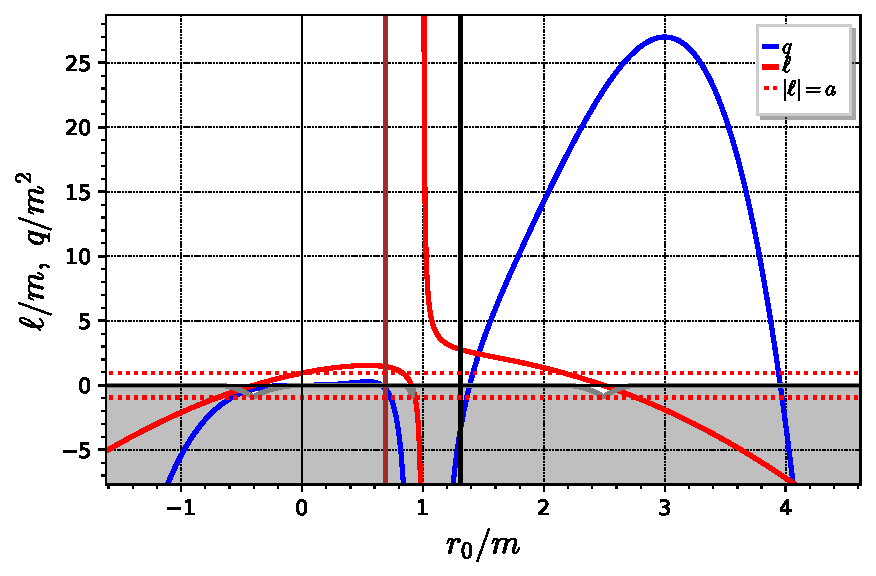
\includegraphics[width=0.49\textwidth]{gik_spher_orb_exist.pdf}\
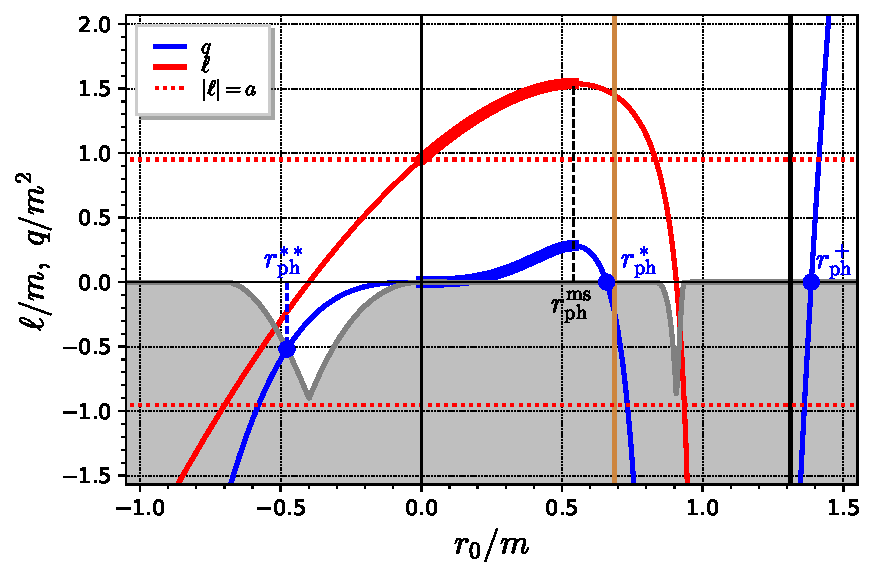
\includegraphics[width=0.49\textwidth]{gik_spher_orb_exist_zoom.pdf}}
\caption[]{\label{f:gik:spher_orb_exist} \footnotesize
Functions $\ell_{\rm c}(r_0)$ (in red) and $q_{\rm c}(r_0)$ (in blue) giving the reduced angular momentum
and reduced Carter constant of a spherical photon orbit of radius $r_0$,
according to Eqs.~(\ref{e:gik:spher_ell_r0}) and (\ref{e:gik:spher_q_r0})
and for $a=0.95\, m$. The right figure is a zoom on the part
$-m\leq r_0 \leq 3m/2$. The thick vertical lines
mark the two horizons: $\Hor$ (black) and $\Hor_{\rm in}$ (light brown).
The horizontal dotted lines mark the boundary of the region $|\ell|<a$,
where $q$ can take negative values. Values of $q$ in the grey zone
are unphysical, i.e. do not fulfil the conditions (\ref{e:gik:q_constraints}),
so that only values of $r_0$ for which the blue curve lies
above the grey zone correspond to spherical photon orbits. This occurs
for $r_{\rm ph}^{**} \leq r_0 \leq r_{\rm ph}^*$ and $r_{\rm ph}^+ \leq r_0 \leq r_{\rm ph}^-$.
The thick segments of the $\ell$ and $q$ curves correspond to stable orbits, for
which $0\leq r_0\leq r_{\rm ph}^{\rm ms}$.
\textsl{[Figure generated by the notebook \ref{s:sam:Kerr_spher_photon_existence}]}
}
\end{figure}

Equations~(\ref{e:gik:spher_ell_r0}) and (\ref{e:gik:spher_q_r0}) provide
the general solution to the system $\mathcal{R}(r_0) = 0$ and $\mathcal{R}'(r_0) = 0$
[Eq.~(\ref{e:gik:R_Rp_r0_zero})], but not all
of them correspond to spherical photon orbits. Indeed, we do not expect
spherical photon orbits to exist for any value of $r_0$, in particular
for $|r_0|\gg m$. Actually, not all values of $q$ given by Eq.~(\ref{e:gik:spher_q_r0})
are permitted, but only those that fulfill the constraints established in
Sec.~\ref{s:gik:th_motion}, namely
\begin{subequations}
\label{e:gik:q_constraints}
\begin{align}
    & q \geq 0 \quad \mbox{if}\  |\ell| \geq a \label{e:gik:q_constraints_1}\\
    & q \geq - \left( a - |\ell| \right) ^2  \quad \mbox{if}\  |\ell| < a . \label{e:gik:q_constraints_2}
\end{align}
\end{subequations}
The solutions $\ell$ and $q$ given by Eqs.~(\ref{e:gik:spher_ell_r0})-(\ref{e:gik:spher_q_r0})
are plotted as functions of $r_0$ for $a=0.95\, m$
in Fig.~\ref{f:gik:spher_orb_exist}, where the
region excluded by (\ref{e:gik:q_constraints}) is colored in grey. Consequently
spherical photon orbits exist only for values of $r_0$ for which the $q$ curve
(in blue) lies above the grey region. We see that this occurs in three intervals:
\be \label{e:gik:spher_orb_range}
    \encadre{ r_0 \in [r_{\rm ph}^{**}, 0) },\quad
    \encadre{ r_0 \in (0, r_{\rm ph}^*] }
    \qand
    \encadre{ r_0 \in [r_{\rm ph}^+, r_{\rm ph}^-] },
\ee
where $r_{\rm ph}^*$, $r_{\rm ph}^+$ and $r_{\rm ph}^-$ are the three (ordered) roots
distinct from $0$ of the equation $q_{\rm c}(r_0) = 0$ (boundary for
condition (\ref{e:gik:q_constraints_1})) and $r_{\rm ph}^{**}$ is the unique
root of the equation $q_{\rm c}(r_0) = - \left( a - |\ell_{\rm c}(r_0)| \right) ^2$ when
$|\ell_{\rm c}(r_0)|  < a$ (boundary for condition (\ref{e:gik:q_constraints_2})).
The above reasoning is based on Fig.~\ref{f:gik:spher_orb_exist}, which has
been drawn for $a=0.95\, m$; however the conclusions (\ref{e:gik:spher_orb_range})
hold for any value of $a$ (see the notebook~\ref{s:sam:Kerr_spher_photon_existence}
for figures with $a=0.5\, m$ or $a=0.998\, m$). We have excluded $r_0=0$
in (\ref{e:gik:spher_orb_range}) because it would yield $\ell = a$ and $q=0$
following Eqs.~(\ref{e:gik:spher_ell_r0})-(\ref{e:gik:spher_q_r0}). But
according to the results of Sec.~\ref{s:gik:th_motion}, such an orbit
would be confined to the equatorial plane, where $r=0$ is not permitted (the ring singularity!).

Given expression (\ref{e:gik:spher_q_r0}) for $q$, we see that
$r_{\rm ph}^*$, $r_{\rm ph}^+$ and $r_{\rm ph}^-$
are the three roots of the cubic equation
\be
r_0(r_0 - 3m)^2 - 4 a^2 m  = 0 .
\ee
We can solve this equation by bringing it to a depressed form in order
to use Viète's formulas (\ref{e:gis:Viete}). However, we may rely on an
already solved equation by noticing the following equivalences:
\begin{eqnarray}
r_0(r_0 - 3m)^2 - 4 a^2 m  = 0  & \iff & r_0 \geq 0 \ \ \mbox{and} \ \
            \sqrt{r_0} | r_0 - 3 m | = 2 a\sqrt{m} \nonumber \\
& \iff &  r_0 \geq 0 \ \ \mbox{and} \ \
    \sqrt{r_0} (r_0 - 3 m ) \pm 2 a \sqrt{m} = 0 \nonumber \\
& \iff &  r_0 \geq 0 \ \ \mbox{and} \ \
    r_0^{3/2} - 3 m r_0^{1/2} \pm 2 a \sqrt{m} = 0 , \nonumber
\end{eqnarray}
where $\pm$ is $+$ for $r_0 \leq 3 m$ and $-$ for $r_0 \geq 3m$.
We recognize the function of $r_0$ which appears in the left-hand side
of Eq.~(\ref{e:gek:cubic_sqrt_r0}). As shown in Sec.~\ref{s:gek:existence_circ_orb},
there are three real roots,
$r_{\rm ph}^*$, $r_{\rm ph}^+$ and $r_{\rm ph}^-$, with
$r_{\rm ph}^*, r_{\rm ph}^+\leq 3m$ ($\pm = +$)
and $r_{\rm ph}^- \geq 3m$ ($\pm = -$). They are given by Eqs.~(\ref{e:gek:def_r_star})
and (\ref{e:gek:def_r_min_pm}):
\be \label{e:gik:rph_s}
   \encadre{ r_{\rm ph}^* := 4m\cos^2 \left[ \frac{1}{3} \arccos\left(-\frac{a}{m} \right)  + \frac{4\pi}{3} \right] } .
\ee
\be \label{e:gik:rph_pm}
   \encadre{ r_{\rm ph}^\pm := 4m\cos^2 \left[ \frac{1}{3} \arccos\left( \mp \frac{a}{m} \right) \right] }
\ee
As for $r_{\rm ph}^{**}$, since $q_{\rm c}(r_0) = - (a - |\ell_{\rm c}(r_0)|)^2$ with
$|\ell_{\rm c}(r_0)|  < a$ occurs in a region where $\ell_{\rm c}(r_0) < 0$ (cf. Fig.~\ref{f:gik:spher_orb_exist}),
we get that $r_{\rm ph}^{**}$ is a solution of the equation
$q_{\rm c}(r_0) = - (a + \ell_{\rm c}(r_0))^2$. Given expressions (\ref{e:gik:spher_ell_r0}) and (\ref{e:gik:spher_q_r0})
for respectively $\ell_{\rm c}(r_0)$ and $q_{\rm c}(r_0)$, we get that $r_{\rm ph}^{**}$ is a root of the cubic
equation
\be \label{e:gik:cubic_rph_ss}
    2 r_0^3 - 3 m r_0^2 + a^2 m = 0 .
\ee
By the change of variable $r_0 =: x + m/2$, we turn this equation into a depressed one:
\[
    x^3  - \frac{3}{4} m^2 x + \frac{m}{2} \left(a^2 - \frac{m^2}{2} \right) = 0 ,
\]
i.e. $x^3 + px + q = 0$, with $p:= -3m^2/4$ and $q:=(m/2)(a^2 - m^2/2)$.
The discriminant is $-(4 p^3 + 27 q^2) = 27 a^2 m^2 (m^2 - a^2)/4 \geq 0$. The three roots
$(x_k)_{k\in\{0,1,2\}}$ are then all real and are given by Viète's formula (\ref{e:gis:Viete}).
Only the root $x_1$ leads to a negative value of $r_0$, which is the value we
are looking for (cf. Fig.~\ref{f:gik:spher_orb_exist}). Viète's formula (\ref{e:gis:Viete})
with $k=1$ yields
\[
    x_1 = m \cos\left[ \frac{1}{3} \arccos\left(1 - 2 \frac{a^2}{m^2} \right) + \frac{2\pi}{3} \right]
        = m \cos\left[ \frac{2}{3} \arcsin\left(\frac{a}{m}\right) + \frac{2\pi}{3} \right] ,
\]
from which we obtain
\be \label{e:gik:rph_ss}
   \encadre{ r_{\rm ph}^{**} = \frac{m}{2} + m \cos\left[ \frac{2}{3} \arcsin\left(\frac{a}{m}\right) + \frac{2\pi}{3} \right] } .
\ee

\begin{figure}
\centerline{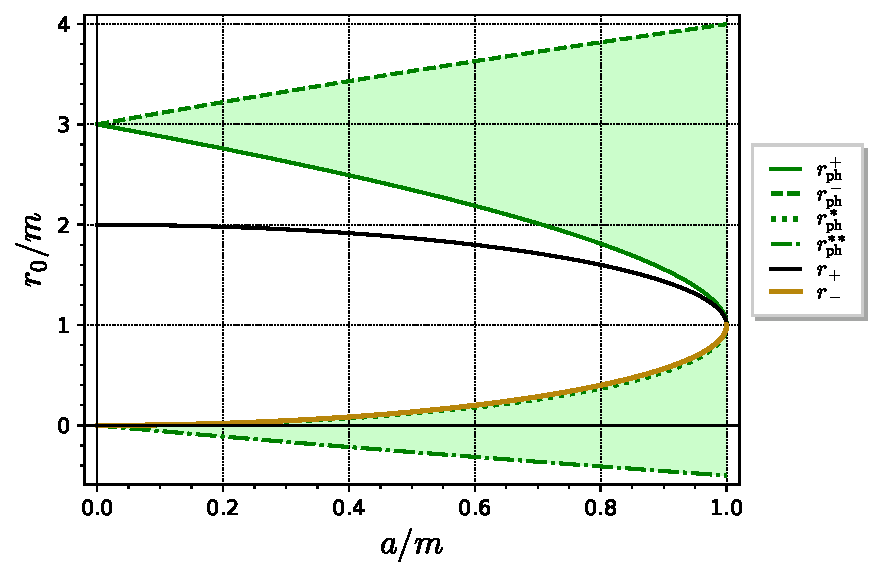
\includegraphics[width=0.75\textwidth]{gik_spher_orb_range.pdf}}
\caption[]{\label{f:gik:spher_orb_range} \footnotesize
Domain of existence of spherical photon orbits in the $(a, r_0)$ plane
(in green). The boundaries of the domain are the radii
$r_{\rm ph}^{**}$, $r_{\rm ph}^*$, $r_{\rm ph}^+$ and $r_{\rm ph}^-$
given by Eqs.~(\ref{e:gik:rph_ss}), (\ref{e:gik:rph_s}) and (\ref{e:gik:rph_pm}).
The shaded area correspond to stable spherical orbits; its upper boundary
(blue curve)
is the radius $r_{\rm ph}^{\rm ms}$ given by Eq.~(\ref{e:gik:r_ph_mb}).
The black curve indicates the black hole horizon $\Hor$ and the light brown one
the inner horizon $\Hor_{\rm in}$.
\textsl{[Figure generated by the notebook \ref{s:sam:Kerr_spher_photon_existence}]}
}
\end{figure}

The four critical radii $r_{\rm ph}^{**}$, $r_{\rm ph}^*$, $r_{\rm ph}^+$ and $r_{\rm ph}^-$
are plotted in terms of $a$ in Fig.~\ref{f:gik:spher_orb_range}. We notice that
\be \label{e:gik:r_crit_order}
  \encadre{  - \frac{m}{2} \leq r_{\rm ph}^{**} \leq 0 \leq r_{\rm ph}^* \leq r_- \leq m \leq r_+ \leq r_{\rm ph}^+
    \leq 3 m \leq r_{\rm ph}^- \leq 4 m },
\ee
with the limits (\ref{e:gek:lim_rph_pm}) and (\ref{e:gek:lim_rph_s}). In addition,
\be
    \lim_{a\to 0} r_{\rm ph}^{**} = 0 \qand
    \lim_{a\to m} r_{\rm ph}^{**} = - \frac{m}{2} .
\ee
As already stressed in Sec.~\ref{s:gek:existence_circ_orb}, $r_{\rm ph}^*$ is lower than, but very close to,
the inner horizon radius $r_{-}$, with  $\max (r_- - r_{\rm ph}^*) \simeq 0.032 \, m$,
achieved for $a\simeq 0.9 \, m$.
In view of the above inequalities and the ranges (\ref{e:gik:spher_orb_range}), we conclude that
\begin{greybox}
Spherical photon orbits with $E\neq 0$ exist in two regions of Kerr spacetime:
\begin{itemize}
\item orbits with $r_0\in [r_{\rm ph}^{**}, 0) \cup (0, r_{\rm ph}^*]$ are located in $\M_{\rm III}$;
we shall call them the \defin{inner spherical photon orbits}\index{inner!spherical photon orbit}\index{spherical!photon orbit!inner --}\index{photon!orbit!inner spherical --};
\item orbits with $r_0 \in [r_{\rm ph}^+, r_{\rm ph}^-]$ are located in $\M_{\rm I}$;
we shall call them the \defin{outer spherical photon orbits}\index{outer!spherical photon orbit}\index{spherical!photon orbit!outer --}\index{photon!orbit!outer spherical --}.
\end{itemize}
\end{greybox}

\subsubsection{Sign of $E$}

All $E\neq 0$ spherical photon orbits lie in $\M_{\rm I}\cup\M_{\rm III}$. We may then apply
the general result (\ref{e:gek:future_directed_Carter}) to them. Since $L = E \ell$, we get
$E (r_0^2 + a^2 - a \ell) > 0$.
Hence, using formula~(\ref{e:gik:spher_ell_r0}) for $\ell$,
\begin{align}
E > 0 & \iff r_0^2 + a^2 - a \ell > 0 \nonumber \\
      & \iff \frac{r_0 \Delta_0}{r_0 - m} > 0 \nonumber \\
      & \iff \frac{r_0}{r_0 - m} > 0  \nonumber \\
      & \iff r_0 > m \ \mbox{or}\ r_0 < 0 , \nonumber
\end{align}
where the third line follows from $\Delta_0 > 0$ in $\M_{\rm I}\cup\M_{\rm III}$.
In view of (\ref{e:gik:r_crit_order}), we conclude that
\begin{greybox}
All outer spherical photon orbits have $E>0$, as well as inner spherical photon
orbits with $r_0\in[r_{\rm ph}^{**}, 0)$, %]$
while inner spherical photon orbits with $r_0\in(0, r_{\rm ph}^*]$
have $E<0$.
\end{greybox}

\subsection{Latitudinal motion} \label{s:gik:spher_latitudinal}

The latitudinal motion of spherical photon orbits is
deduced from the general results of Sec.~\ref{s:gik:th_motion},
where geodesics with $\ell=0$ appear as a special case. We thus treat this
case first.

\subsubsection{Polar spherical photon orbits}

We see on Fig.~\ref{f:gik:spher_orb_exist} that the reduced conserved
angular momentum $\ell$ (red curve) vanishes at two
places in the physically allowed range of $r_0$,
i.e. where the blue curve lies above the grey region:
$r_0=r_{\rm ph}^{\rm pol,in}$ and $r_0=r_{\rm ph}^{\rm pol}$
with $r_{\rm ph}^{**} < r_{\rm ph}^{\rm pol,in} < 0$ and
$r_{\rm ph}^+ < r_{\rm ph}^{\rm pol} < r_{\rm ph}^-$.
The value $r_{\rm ph}^{\rm pol,in}$ (resp. $r_{\rm ph}^{\rm pol}$)
corresponds thus to inner (resp. outer) spherical orbits.
The results of Sec.~\ref{s:gik:th_motion} show that these orbits
are the only ones that encounter the rotation axis; moreover, they
cross it repeatedly.
We therefore call them
\defin{polar spherical photon orbits}\index{polar!spherical photon orbits}.

The values of $r_{\rm ph}^{\rm pol,in}$ and
$r_{\rm ph}^{\rm pol}$ are obtained by solving $\ell_{\rm c}(r_0) = 0$,
with $\ell_{\rm c}(r_0)$ given by Eq.~(\ref{e:gik:spher_ell_r0}). We get the cubic
equation $r_0^3 - 3 m r_0^2 + a^2 r_0 + a^2 m = 0$. Setting $r_0 =: x + m$ reduces
it to the depressed cubic $x^3 + p x + q = 0$, with $p := a^2 - 3 m^2$
and $q := 2m (a^2 - m^2)$. The discriminant $\mathit{\Delta} = - 4 p^3 - 27 q^2$
being positive, the solutions are provided by Viète's formulas, Eq.~(\ref{e:gis:Viete}),
with $k=0$ and $k=1$ ($k=2$ leads to the third root of $\ell_{\rm c}(r_0)$ seen on
Fig.~\ref{f:gik:spher_orb_exist}, which lies
in the unphysical range of $r_0$ --- blue curve in the grey region):
\begin{subequations}
\begin{align}
    r_{\rm ph}^{\rm pol} & = m + 2 \sqrt{m^2 - \frac{a^2}{3}}
        \cos\left[ \frac{1}{3}\arccos \left(
        \frac{m(m^2 - a^2)}{\left( m^2 - {a^2}/{3} \right) ^{3/2}} \right) \right]
        \label{e:gik:rph_pol} \\
    r_{\rm ph}^{\rm pol,in} & = m + 2 \sqrt{m^2 - \frac{a^2}{3}}
        \cos\left[ \frac{1}{3}\arccos \left(
        \frac{m(m^2 - a^2)}{\left( m^2 - {a^2}/{3} \right) ^{3/2}} \right) + \frac{2\pi}{3} \right] .
\end{align}
\end{subequations}
As a function of $a$, $r_{\rm ph}^{\rm pol}$ decays monotonically from
$\lim_{a\to 0} r_{\rm ph}^{\rm pol} = 3 m$ to
$\lim_{a\to m} r_{\rm ph}^{\rm pol} = ( 1 + \sqrt{2}) m \simeq 2.414214\, m$,
while $r_{\rm ph}^{\rm pol,in}$ decays monotonically from
$\lim_{a\to 0} r_{\rm ph}^{\rm pol,in} = 0$ to
$\lim_{a\to m} r_{\rm ph}^{\rm pol,in} = (1 - \sqrt{2}) m \simeq -0.414214\, m$.

\subsubsection{Sign of $\ell$ and $L$}

For spherical orbits with $\ell\neq 0$,
the sign of $\ell$ is deduced from expression (\ref{e:gik:spher_ell_r0}),
whose numerator has a sign governed by the position of $r_0$ with respect to the
roots $r_{\rm ph}^{\rm pol,in}$ and $r_{\rm ph}^{\rm pol}$ determined above and whose denominator is positive iff $r_0 > m$, which occurs
only for outer spherical orbits. We get then
\begin{greybox}
\begin{itemize}
\item Outer spherical orbits with $r_0 \in [r_{\rm ph}^+, r_{\rm ph}^{\rm pol})$ %]$
have $\ell > 0$;
\item outer spherical orbits with $r_0 \in (r_{\rm ph}^{\rm pol}, r_{\rm ph}^-]$ %]$
have $\ell < 0$;
\item inner spherical orbits with $r_0 \in (r_{\rm ph}^{\rm pol,in}, r_{\rm ph}^*]$
have $\ell > 0$;
\item inner spherical orbits with $r_0 \in [r_{\rm ph}^{**}, r_{\rm ph}^{\rm pol,in})$ %]$
have $\ell < 0$.
\end{itemize}
\end{greybox}
The sign of $L$ is deduced from that of $\ell = L/E$ by combining with the sign of $E$ obtained
in Sec.~\ref{s:gik:spher_existence}.

\subsubsection{Latitudinal motion}

By applying the results of Sec.~\ref{s:gik:th_motion}, we get

\begin{greybox}
\begin{itemize}
\item All outer spherical photon orbits with $r_0\not\in \left\{r_{\rm ph}^+, r_{\rm ph}^-\right\}$ and the inner ones with $r_0\in (0, r_{\rm ph}^{*})$
have $q>0$ (cf. Fig.~\ref{f:gik:spher_orb_exist}); they therefore cross the equatorial plane.
Moreover,
\begin{itemize}
\item those with $r_0 = r_{\rm ph}^{\rm pol}$ (outer polar spherical photon orbits)
have $\ell=0$
and cross repeatedly the rotation axis and the equatorial plane, with $\th$
taking all values in the range $[0,\pi]$;
\item those with $r_0 \neq r_{\rm ph}^{\rm pol}$
oscillate about the equatorial plane, having two $\th$-turning points
symmetrical about it, at $\th=\th_{\rm m}$ and $\th=\pi-\th_{\rm m}$, with
$\th_{\rm m}$ given by Eq.~(\ref{e:gik:th0}),
in which $\ell$ and $q$ are to be considered as the functions
(\ref{e:gik:spher_ell_r0})-(\ref{e:gik:spher_q_r0}) of $r_0$.
\end{itemize}
\item Inner spherical photon orbits with $r_0 \in (r_{\rm ph}^{**}, 0)$
have $q<0$ (cf. right panel of Fig.~\ref{f:gik:spher_orb_exist}); they are thus vortical
and never encounter the equatorial plane. Moreover,
\begin{itemize}
\item those with $r_0 = r_{\rm ph}^{\rm pol, in}$ (inner polar spherical photon orbits)
have $\ell=0$ and oscillate about the rotation axis,
with a $\th$-turning point at
$\th=\th_{\rm v}$ (Northern hemisphere) or $\th = \pi - \th_{\rm v}$ (Southern hemisphere),
where $\th_{\rm v}$
is given by Eq.~(\ref{e:gik:thv_ell_zero}) in which $q$ is to be considered
as the function (\ref{e:gik:spher_q_r0}) of $r_{\rm ph}^{\rm pol, in}$.
\item those with $r_0 \neq r_{\rm ph}^{\rm pol, in}$ neither encounter the rotation axis nor the
equatorial plane, having
either $\th\in[\th_{\rm m}, \th_{\rm v}]$ (Northern hemisphere)
or $\th\in[\pi-\th_{\rm v}, \pi-\th_{\rm m}]$ (Southern hemisphere), with
$\th_{\rm m}$ and $\th_{\rm v}$ given by Eqs.~(\ref{e:gik:th0}) and (\ref{e:gik:th1_general}), in which
$\ell$ and $q$ are to be considered as the functions
(\ref{e:gik:spher_ell_r0})-(\ref{e:gik:spher_q_r0}) of $r_0$.
\end{itemize}
\end{itemize}
Spherical photon orbits at $r_0 = r_{\rm ph}^{**}$, $r_{\rm ph}^*$, $r_{\rm ph}^+$ or $r_{\rm ph}^-$,
which have been excluded from the above list,
will be discussed in details in Sec.~\ref{s:gik:circular_orbits}.
\end{greybox}

In addition, we have
\begin{greybox}
For a spherical photon orbit, $\th$ is either a constant or a periodic function
of the affine parameter $\lambda$, the period being
\be
    \Lambda_\th = \frac{2}{|E|}\int_{\th_{\rm min}}^{\th_{\rm max}}
    \frac{r_0^2 + a^2 \cos^2\th}{\sqrt{\tilde{\Theta}(\th)}} \, \D \th ,
\ee
with $(\th_{\rm min}, \th_{\rm max}) = (0, \pi)$ (outer polar orbit),
$(0, \th_{\rm v})$ (Northern inner polar orbit),
$(\pi-\th_{\rm v}, \pi)$ (Southern inner polar orbit),
$(\th_{\rm m}, \pi- \th_{\rm m})$
(non-polar orbit with $r_0\in (0, r_{\rm ph}^{*}) \cup (r_{\rm ph}^+, r_{\rm ph}^-)$),
$(\th_{\rm m}, \th_{\rm v})$
(Northern non-polar vortical inner orbit) or
$(\pi-\th_{\rm v}, \pi-\th_{\rm m})$
(Southern non-polar vortical inner orbit).
\end{greybox}
\begin{proof}
Swiching from the Mino parameter $\lambda'$ to the affine parameter $\lambda$
via the relation (\ref{e:gek:def_Mino_time}) with $r(\lambda)=r_0$, we may
rewrite the equation of motion (\ref{e:gik:dthdl_Mino}) as
\[
    \left( \derd{\th}{\lambda} \right)^2 + \mathcal{V}(\th) = 0,
    \quad\mbox{with}\
    \mathcal{V}(\th) :=
    - \frac{E^2 \tilde{\Theta}(\th)}{(r_0^2 + a^2 \cos^2\th)^2} .
\]
This is the 1-dimensional equation of motion in the potential well $\mathcal{V}$.
It is then clear that $\th(\lambda)$ is a periodic function. The
period $\Lambda_\th$ is evaluated by integrating
$\D\lambda = \eps_\th (r_0^2 + a^2 \cos^2\th)^2 / (|E| \sqrt{\tilde{\Theta}(\th)})$
over a ``round-trip'' to the same values of $\th$ and $\D\th/\D\lambda$.
\end{proof}

\begin{remark}
The azimuthal coordinate
$\ph$ is not a periodic function of the affine parameter $\lambda$ in general,
nor of the Mino paramater $\lambda'$. An exception regards polar spherical
geodesics, since setting $\ell=0$ in the equation of motion (\ref{e:gik:dphdl_Mino}) results
in $\D\ph/\D\lambda' = \mathrm{const}$, so that $\ph$ is a periodic function of $\lambda'$
(but still not of $\lambda$).
\end{remark}

\begin{figure}
\centerline{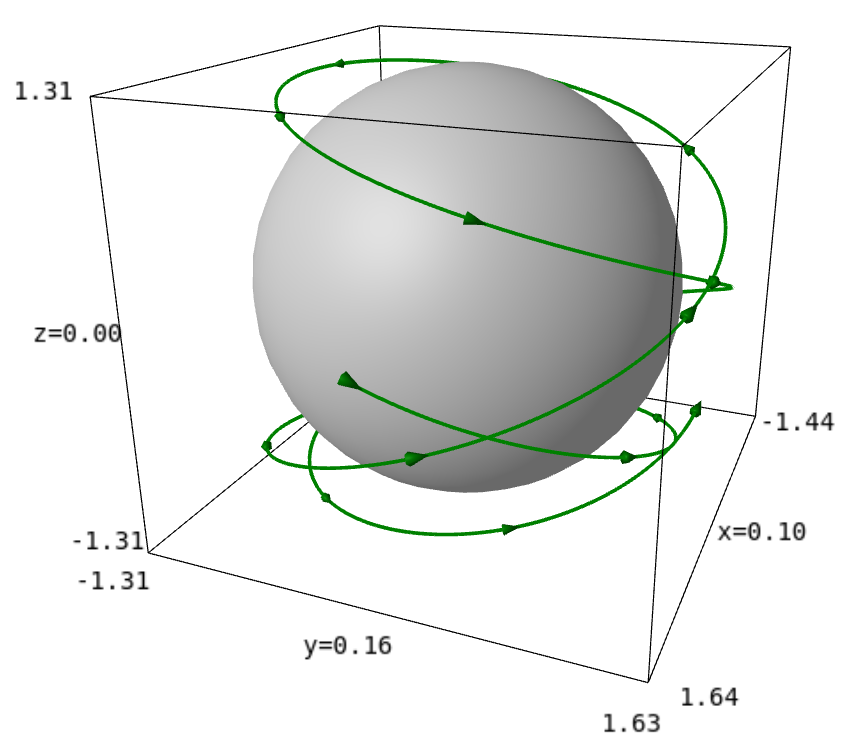
\includegraphics[width=0.48\textwidth]{gik_spher_3d_r_16_l077.png}\
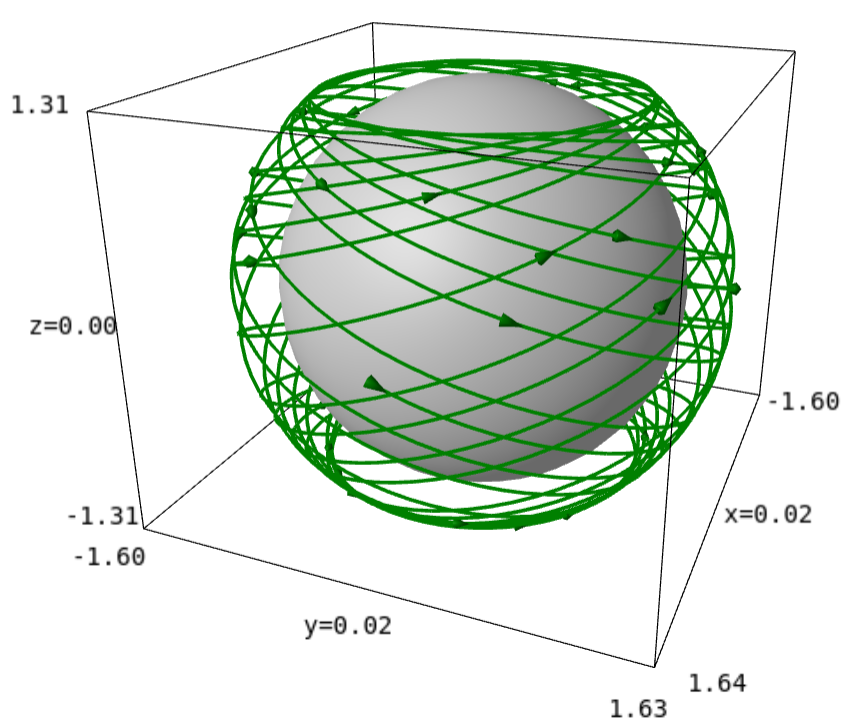
\includegraphics[width=0.49\textwidth]{gik_spher_3d_r_16_l700.png}}
\caption[]{\label{f:gik:spher_3d_r_16} \footnotesize
Spherical photon orbit at $r_0=1.6 \, m$ around a Kerr black hole with
$a=0.95\, m$, depicted in terms of the Cartesian Boyer-Lindquist coordinates
$(x,y,z)$ defined by Eq.~(\ref{e:gek:Cartesian_BL}) and scaled in units of $m$.
The geodesic starts at $\lambda=0$ and $\ph=0$ in the equatorial plane, in the direction
of the Southern hemisphere ($\D\th/\D\lambda>0$).
The left panel corresponds to $0 \leq \lambda \leq 7.7\, m/E$,
while the right one extends the range to $0 \leq \lambda \leq 70\, m/E$.
The grey sphere is the black hole event horizon.
\textsl{[Figure generated by the notebook \ref{s:sam:Kerr_spher_null_geod}]}
}
\end{figure}

\begin{figure}
\centerline{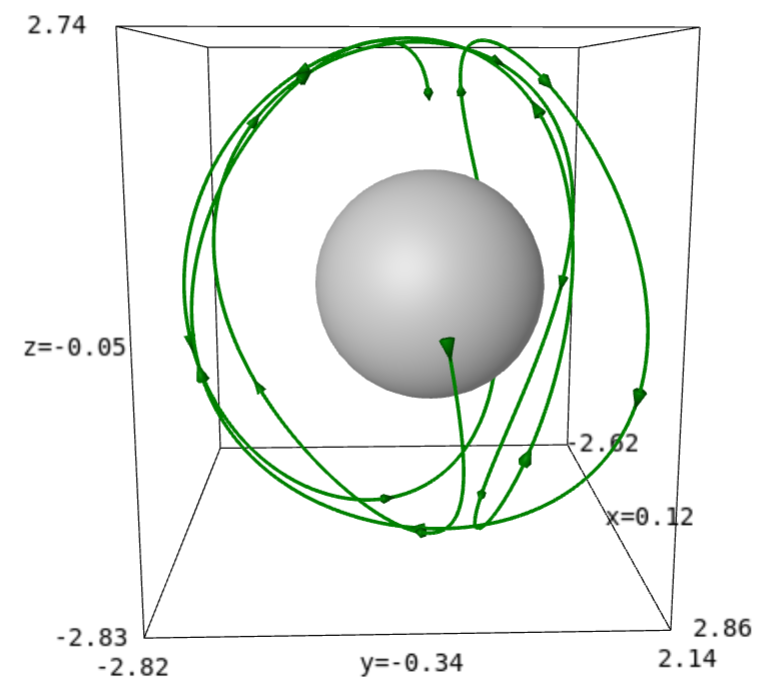
\includegraphics[width=0.49\textwidth]{gik_spher_3d_r_28.png}\
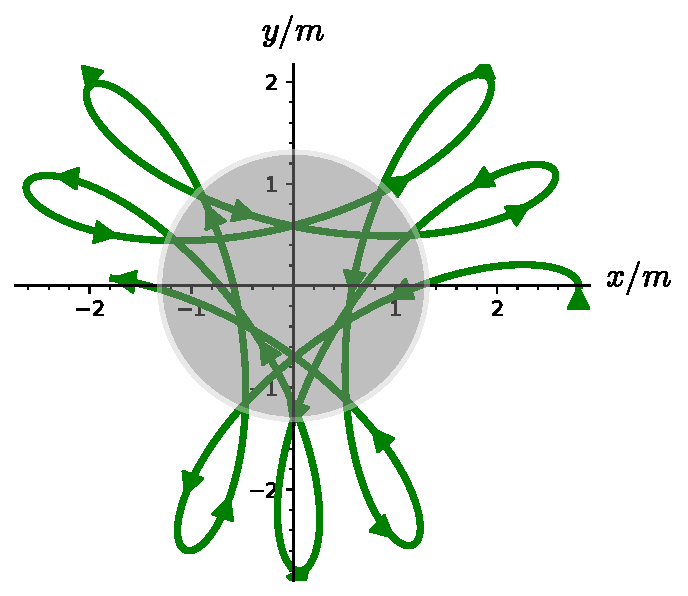
\includegraphics[width=0.49\textwidth]{gik_spher_3d_r_28_xy.pdf}}
\caption[]{\label{f:gik:spher_3d_r_28} \footnotesize
Spherical photon orbit at $r_0=2.8 \, m$ around a Kerr black hole with
$a=0.95\, m$, depicted in terms of the Cartesian Boyer-Lindquist coordinates
$(x,y,z)$ defined by Eq.~(\ref{e:gek:Cartesian_BL}) and scaled in units of $m$,
with the grey sphere representing the black hole event horizon.
The right panel depicts the projection of the orbit onto the $xy$-plane
(the overlap with the grey area is a mere projection effect, since of course
the orbit never crosses the event horizon).
The geodesic starts at $\lambda=0$ and $\ph=0$ in the equatorial plane, in the direction
of the Southern hemisphere. The plotted range is $0 \leq \lambda \leq 38\, m/E$.
\textsl{[Figure generated by the notebook \ref{s:sam:Kerr_spher_null_geod}]}
}
\end{figure}

\begin{figure}
\centerline{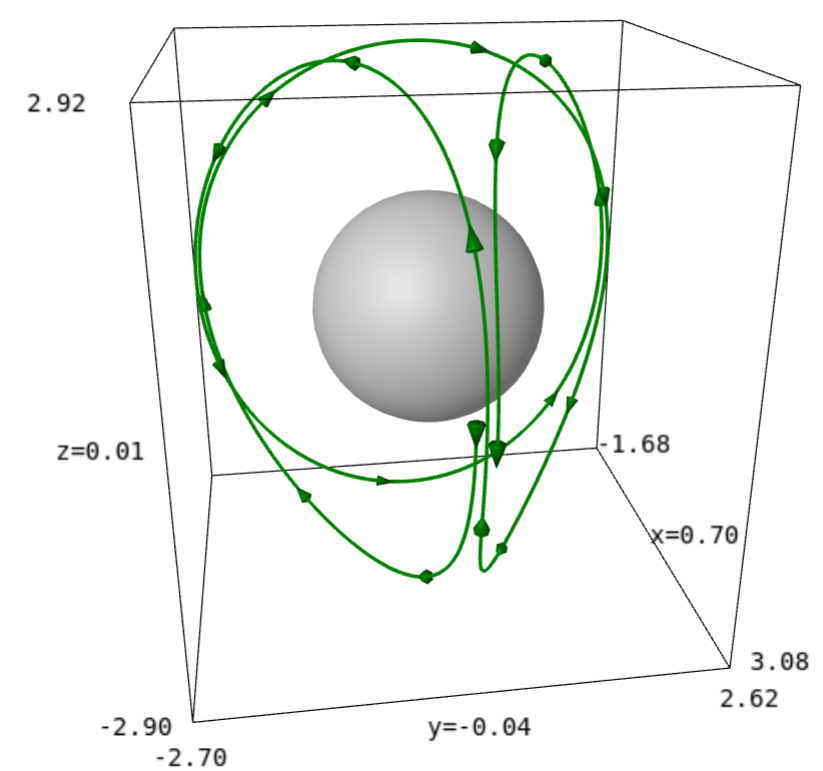
\includegraphics[width=0.49\textwidth]{gik_spher_3d_r_30.png}\
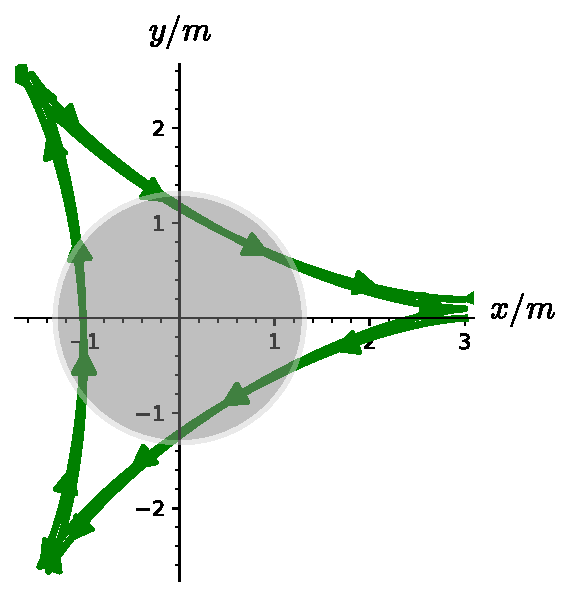
\includegraphics[width=0.4\textwidth]{gik_spher_3d_r_30_xy.pdf}}
\caption[]{\label{f:gik:spher_3d_r_30} \footnotesize
Same as in Fig.~\ref{f:gik:spher_3d_r_28}  but for a
spherical photon orbit at $r_0=3 m$, with
$0 \leq \lambda \leq 32\, m/E$.
\textsl{[Figure generated by the notebook \ref{s:sam:Kerr_spher_null_geod}]}
}
\end{figure}

\begin{figure}
\centerline{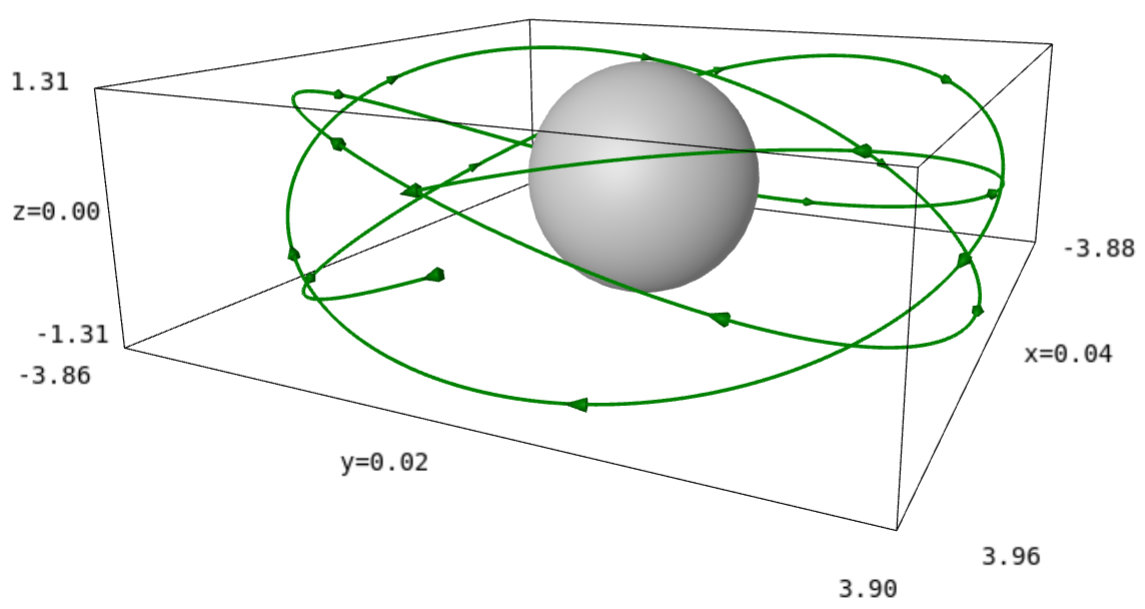
\includegraphics[width=0.58\textwidth]{gik_spher_3d_r_39.png}\
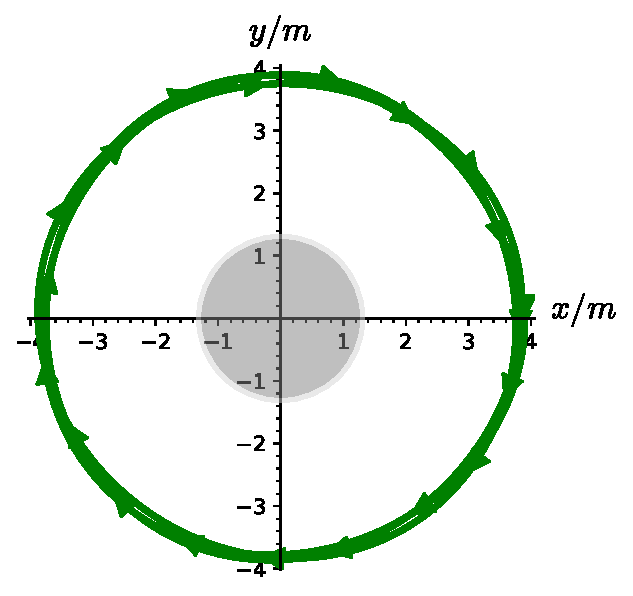
\includegraphics[width=0.4\textwidth]{gik_spher_3d_r_39_xy.pdf}}
\caption[]{\label{f:gik:spher_3d_r_39} \footnotesize
Same as in Fig.~\ref{f:gik:spher_3d_r_28}  but for a
spherical photon orbit at $r_0=3.9\, m$, with
$0 \leq \lambda \leq 55\, m/E$.
\textsl{[Figure generated by the notebook \ref{s:sam:Kerr_spher_null_geod}]}
}
\end{figure}

\begin{example}[Outer spherical photon orbits] \label{x:gik:outer_spher}
Let us consider a Kerr black hole with $a=0.95\, m$ (same value as in
Fig.~\ref{f:gik:spher_orb_exist}). The event and inner horizon radii
are $r_+ = 1.312\, m$ and $r_- = 0.688\, m$ and one has
$r_{\rm ph}^{**} = - 0.478\, m$, $r_{\rm ph}^{*} = 0.658\, m$,
$r_{\rm ph}^+ = 1.386\, m$ and $r_{\rm ph}^- = 3.955\, m$.
Some outer spherical photon orbits are plotted in
Figs.~\ref{f:gik:spher_3d_r_16}--\ref{f:gik:spher_3d_r_39}
for various values of $r_0$:
\begin{itemize}
\item $r_0 = 1.6\, m$ (Fig.~\ref{f:gik:spher_3d_r_16}): this orbit
has $\ell = 2.171\, m$, $q=5.976\, m^2$, $\th_{\rm m} = 0.706\;{\rm rad}$ and $\D\ph/\D\lambda > 0$;
\item $r_0 = 2.8\, m$ (Fig.~\ref{f:gik:spher_3d_r_28}): this orbit
has $\ell = -1.089\, m$, $q=26.260\, m^2$ and $\th_{\rm m} = 0.206\;{\rm rad}$;
$\ph(\lambda)$ is not a monotonous function (cf. the projection onto the $xy$-plane):
$\D\ph/\D\lambda < 0$ almost everywhere, except
near the equator, where the Lense-Thirring effect\index{Lense-Thirring effect} (cf. Sec.~\ref{s:gek:Lense-Thirring})
is the strongest\footnote{This can be seen
by considering the limit $\th\to\pi/2$ in Eq.~(\ref{e:gik:dphdl_Mino}).} and
enforces $\D\ph/\D\lambda > 0$;
\item $r_0 = 3 m$ (Fig.~\ref{f:gik:spher_3d_r_30}): this orbit
has $\ell = -1.9\, m$, $q=27\, m^2$, $\th_{\rm m} = 0.346\;{\rm rad}$ and
$\D\ph/\D\lambda \leq 0$, with $\D\ph/\D\lambda = 0$ in the equatorial plane,
as it can be easily checked by plugging $r=3m$, $\th=\pi/2$ as well as
the above values of $\ell$ and $q$ into Eq.~(\ref{e:gik:dphdl_Mino});
this orbit maximizes the value of $q$ among all spherical photon orbits
(cf. Fig.~\ref{f:gik:spher_orb_exist} and Eq.~(\ref{e:gik:spher_max_q}) below);
\item $r_0 = 3.9\, m$ (Fig.~\ref{f:gik:spher_3d_r_39}): this orbit
has $\ell = -6.574\, m$, $q=3.525\, m^2$, $\th_{\rm m} = 1.290\;{\rm rad}$
and $\D\ph/\D\lambda < 0$.
\end{itemize}
\end{example}

The next example is devoted to inner spherical photon orbits. The
Cartesian Boyer-Lindquist coordinates $(t,x,y,z)$ are not well suited to
depict these orbits, in particular those that have $r<0$. We could
use O'Neill exponential coordinates\index{O'Neill!coordinates}, as in Fig.~\ref{f:gik:zero_ener_merid}.
However, we are going to use instead the radial coordinate $\hat{r}$ and the
associated Cartesian-type coordinates $(\hat{x}, \hat{y}, \hat{z})$ defined
by
\begin{subequations}
\label{e:gik:def_hat_coord}
\begin{align}
    & \hat{r} := \frac{1}{2} \left( r + \sqrt{r^2 + 4m^2} \right)  \\
    & \hat{x} := \hat{r}\sin\th\cos\ph,\quad
      \hat{y} := \hat{r}\sin\th\sin\ph,\quad
      \hat{z} := \hat{r}\cos\th .
\end{align}
\end{subequations}
As O'Neill coordinates, this brings the whole range
$(-\infty,+\infty)$ for $r$
to $(0,+\infty)$ for $\hat{r}$, with $\hat{r}\to 0$ corresponding to $r\to -\infty$.
Contrary to O'Neill coordinate $\mathrm{e}^{r/m}$, the
coordinate $\hat{r}$ does not enlarge too much the region exterior
to the black hole, which makes it better suited for plots covering both
the black hole interior and exterior, as in Fig.~\ref{f:gik:spo_meridional} below.
Note that in $\M_{\rm I}$, $\hat{r}$ is asymptotically equivalent to $r$:
$\hat{r} \sim r $ as $r\to + \infty$.

\begin{figure}
\centerline{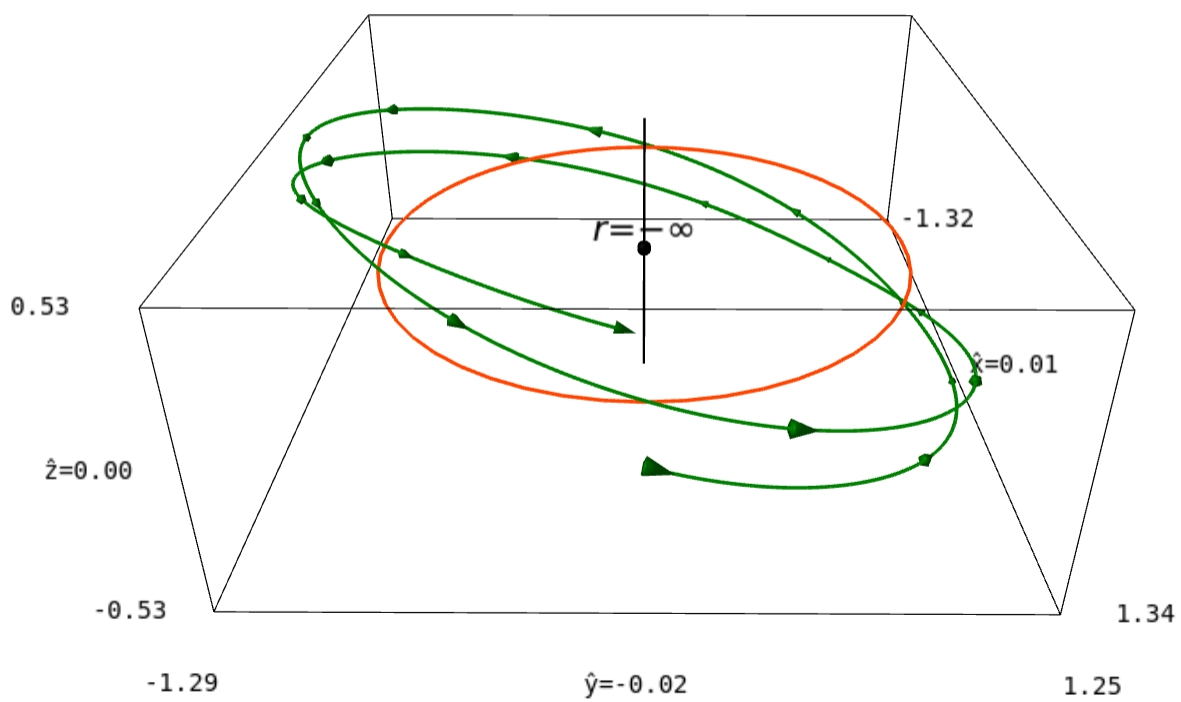
\includegraphics[width=0.48\textwidth]{gik_spher_3d_ms_l030.png}\
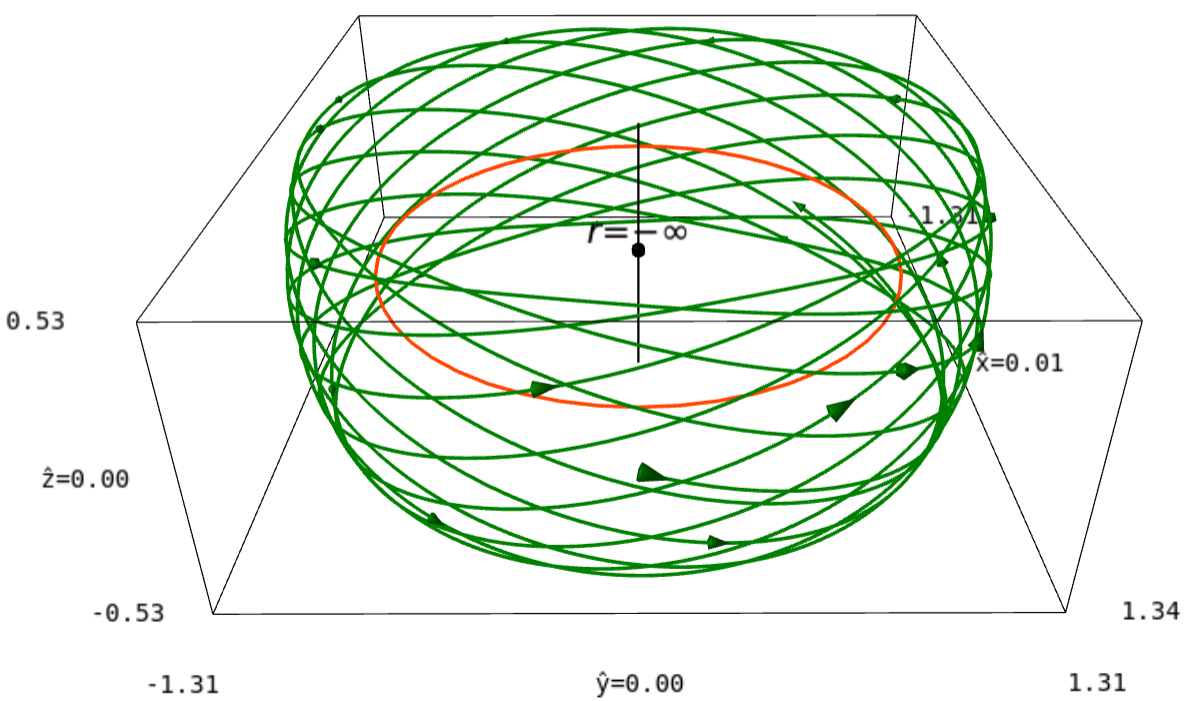
\includegraphics[width=0.49\textwidth]{gik_spher_3d_ms_l200.png}}
\caption[]{\label{f:gik:spher_3d_ms} \footnotesize
Marginally stable spherical photon orbit inside a Kerr black hole with
$a=0.95\, m$, depicted in terms of the coordinates
$(\hat{x},\hat{y},\hat{z})$ defined by Eq.~(\ref{e:gik:def_hat_coord}) and scaled in units of $m$.
The geodesic is located at $r_0 = 0.540\, m$ and starts at $\lambda=0$ and $\ph=0$ in the equatorial plane, in the direction
of the Southern hemisphere ($\D\th/\D\lambda>0$).
The left panel corresponds to $0 \leq \lambda \leq 3\, m/|E|$,
while the right one extends the range to $0 \leq \lambda \leq 20, m/|E|$.
The orange red circle is the ring singularity and the vertical black line
is the rotation axis, with a black dot marking the asymptotic end $r\to -\infty$.
\textsl{[Figure generated by the notebook \ref{s:sam:Kerr_spher_null_geod}]}
}
\end{figure}

\begin{figure}
\centerline{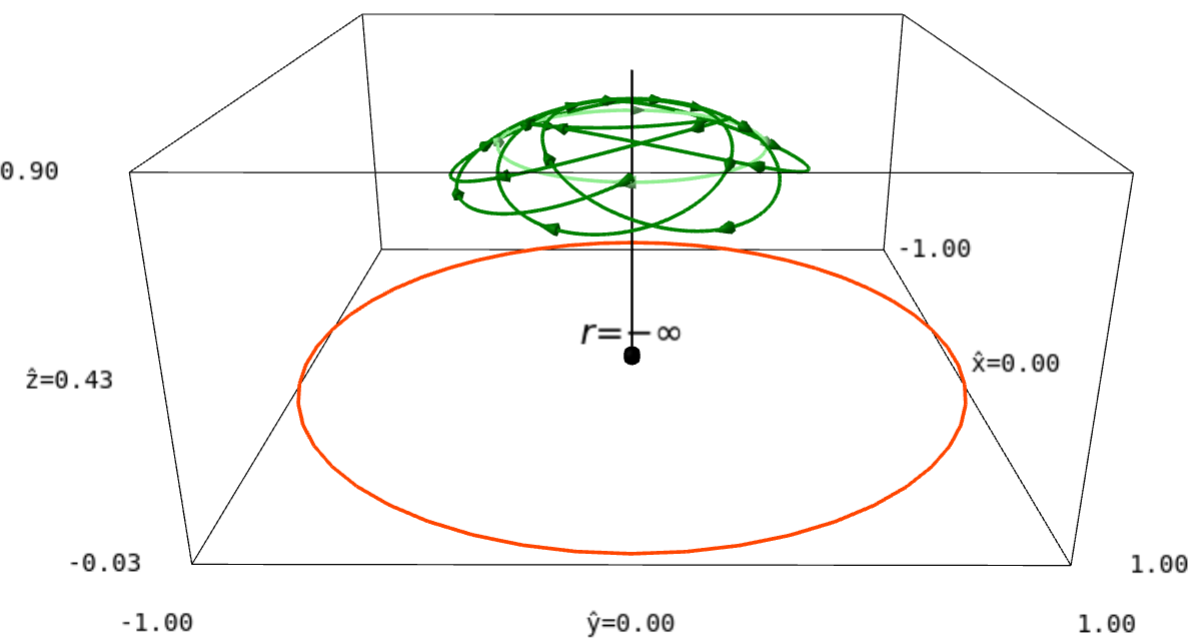
\includegraphics[width=0.7\textwidth]{gik_spher_3d_r_m046.png}}
\caption[]{\label{f:gik:spher_3d_r_m046} \footnotesize
Same as in Fig.~\ref{f:gik:spher_3d_ms} but for a vortical
spherical photon orbit at $r_0=-0.46\, m$, with
$0 \leq \lambda \leq 20\, m/E$. Also shown is the Northern vortical circular photon orbit
at $r = r_{\rm ph}^{**}$ (in light green).
\textsl{[Figure generated by the notebook \ref{s:sam:Kerr_spher_null_geod}]}
}
\end{figure}


\begin{example}[Inner spherical photon orbits]
We consider the same Kerr spacetime as in Example~\ref{x:gik:outer_spher},
i.e. $a=0.95\, m$, but this time, we focus on inner spherical photon orbits:
\begin{itemize}
\item $r_0 = 0.540\, m$ (Fig.~\ref{f:gik:spher_3d_ms}):
this orbit has $\ell = 1.539\, m$, $q=0.282\, m^2$, $\th_{\rm m} = 1.173\;{\rm rad}$
$\D\ph/\D\lambda > 0$, $E<0$ and $L<0$; it is actually a marginally stable
photon orbit ($r_0 = r_{\rm ph}^{\rm ms}$), as we shall see
in Sec.~\ref{s:gik:spher_stability};
\item $r_0 = -0.46\, m$ (Fig.~\ref{f:gik:spher_3d_r_m046}):
this orbit has $\ell = -0.176\, m$, $q=-0.461\, m^2$ (hence it is vortical),
$\th_{\rm m} = 0.282\;{\rm rad}$, $\th_{\rm v} = 0.731\;{\rm rad}$,
$\D\ph/\D\lambda < 0$, $E>0$ and $L<0$;
\item $r_0 = -0.478\, m = r_{\rm ph}^{**}$ (Fig.~\ref{f:gik:spher_3d_r_m046},
light green curve): this orbit has $\ell = -0.229\, m$, $q=-0.519\, m^2$ (hence it is vortical),
$\th_{\rm m} = \th_{\rm v} = \th_{\rm ph}^{**} = 0.514\;{\rm rad}$,
$\D\ph/\D\lambda < 0$, $E>0$ and $L<0$.
\end{itemize}
\end{example}


\begin{figure}
\centerline{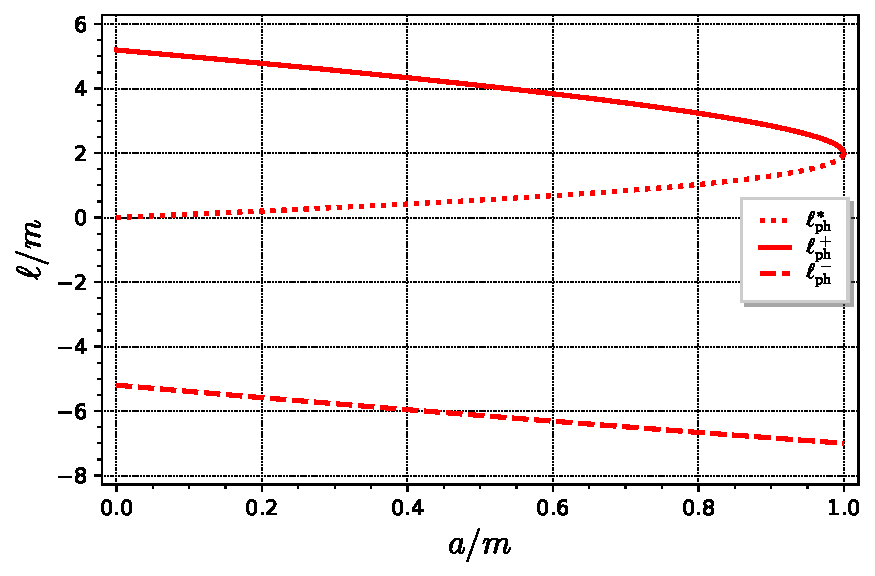
\includegraphics[width=0.6\textwidth]{gik_ell_circ_equat.pdf}}
\caption[]{\label{f:gik:ell_circ_equat} \footnotesize
Reduced angular momentum $\ell$ of the three circular photon orbits in the
equatorial plane, as a function of the Kerr spin parameter $a$.
\textsl{[Figure generated by the notebook \ref{s:sam:Kerr_spher_photon_existence}]}
}
\end{figure}

\subsection{Circular photon orbits} \label{s:gik:circular_orbits}

In any stationary and axisymmetric spacetime, such as the Kerr spacetime, one may
define a \defin{circular photon orbit}\index{circular!photon orbit}\index{photon!orbit!circular --}
as a null geodesic $\Li$ whose tangent vector field $\w{p}=\D\w{x}/\D\lambda$ is a linear combination
of the two Killing vectors $\w{\xi}$ and $\w{\eta}$ generating respectively
the stationarity and the axisymmetry, with a non-vanishing component along $\w{\eta}$:
\be \label{e:gik:def_circular_orbit}
    \w{p} = \alpha \w{\xi} + \beta \w{\eta} ,\quad\mbox{with}\ \beta \neq 0.
\ee
Note that the above definition is independent from any coordinate system.
It is worth to compare Eq.~(\ref{e:gik:def_circular_orbit}) with expression~(\ref{e:gek:4vel_circ_orb}) for the 4-velocity $\w{u} = \mu^{-1}\w{p}$ of a circular timelike orbit in the equatorial plane.

\begin{remark}
Circular photon orbits are sometimes called \defin{light rings}\index{light!ring}\index{ring!light --}
\cite{CunhaH18}.
\end{remark}

In Kerr spacetime, when using coordinates adapted to the spacetime symmetries,
such as Boyer-Lindquist coordinates $(t,r,\th,\ph)$, one has $\w{\xi} = \wpar_t$,
$\w{\eta}=\wpar_\ph$, $\alpha=p^t$, $\beta=p^\ph$ and the definition (\ref{e:gik:def_circular_orbit})
is equivalent to $p^r = \D r/\D\lambda = 0$ and $p^\th = \D\th/\D\lambda = 0$. It follows immediately
that a circular photon orbit is any null geodesic
along which both $r$ and $\th$ are constant. It is thus a spherical photon orbit lying at a constant
value of $\th$.

\begin{remark}
In Schwarzschild spacetime, the photon circular orbits forming the photon sphere
at $r=3m$ (cf. Sec.~\ref{s:ges:null_eff_pot}) do not have $\th=\mathrm{const}$, except
for the orbit in the equatorial plane. However, for a given orbit non-equatorial
orbit on the photon sphere, one may use the spherical symmetry of Schwarzschild spacetime
to perform a change of coordinates $(\th,\ph) \mapsto (\th',\ph')$ such that
$\th' = \mathrm{const}$ is constant for that orbit.
In Kerr spacetime with $a\neq 0$, such
``oblique'' circular orbits cannot exist due to Lense-Thirring precession.
\end{remark}

\begin{example}
The spherical photon orbits with $E=0$ discussed in Sec.~\ref{s:gik:spher_existence},
namely the null generators of the horizons $\Hor$ and $\Hor_{\rm in}$ are
circular photon orbits, since they belong to the family of outgoing principal
null geodesics, which have $\th=\mathrm{const}$.
\end{example}

The spherical photon orbits with $r_0 = r_{\rm ph}^*$, $r_{\rm ph}^+$ and $r_{\rm ph}^-$ have $q=0$
and $|\ell| > a$. According to the results of Sec.~\ref{s:gik:th_motion}, they
necessary lie in the equatorial plane $\th=\pi/2$. They are thus circular.
According to expression~(\ref{e:gik:spher_q_r0}) for $q$, they are the
only circular orbits in the equatorial plane, because the only other root of $q_{\rm c}(r_0)=0$ is $r_0=0$
(see also Fig.~\ref{f:gik:spher_orb_exist}),
which would correspond to the ring singularity.
Let us denote by $\ell_{\rm ph}^*$, $\ell_{\rm ph}^+$ and $\ell_{\rm ph}^-$
the reduced angular momentum $\ell$ of respectively the
circular photon orbit at $r_{\rm ph}^*$, $r_{\rm ph}^+$ and $r_{\rm ph}^-$.
These values of $\ell$ are deduced from Eq.~(\ref{e:gik:spher_ell_r0}) and
are plotted in terms of $a$ in Fig.~\ref{f:gik:ell_circ_equat}.
We have $\ell_{\rm ph}^*>0$, $\ell_{\rm ph}^+>0$ and $\ell_{\rm ph}^-<0$.
Moreover,
\be
    \lim_{a\to 0} \ell_{\rm ph}^+ =  \lim_{a\to 0} \left| \ell_{\rm ph}^- \right|
    = 3\sqrt{3} m \simeq 5.196\, m ,
\ee
in agreement with the Schwarzschild result (\ref{e:ges:b_crit}), while
\be
    \lim_{a\to m} \ell_{\rm ph}^+ =  \lim_{a\to m} \ell_{\rm ph}^* = 2 m,
\ee
in agreement with Eq.~(\ref{e:gik:spher_orb_r0_eq_m}), since
$\lim_{a\to m} r_{\rm ph}^+ = \lim_{a\to m} r_{\rm ph}^* = m$.

The spherical orbits with $r_0 = r_{\rm ph}^{**}$ have
$q < 0$, i.e. are vortical geodesics. Moreover, they fulfill $q=q_{\rm min}=-(a - |\ell|)^2$.
According to the results of Sec.~\ref{s:gik:th_motion}, this corresponds to two orbits at
a fixed value of $\th$, which are symmetrical with respect to the equatorial plane.
They lie at $\th = \th_{\rm ph}^{**}$ (Northern hemisphere) and
$\th = \pi - \th_{\rm ph}^{**}$ (Southern hemisphere), where
$\th_{\rm ph}^{**}$ is given by Eq.~(\ref{e:gik:th_s_ell_over_a}), using
for $\ell$ the value (\ref{e:gik:spher_ell_r0}) with $r_0 = r_{\rm ph}^{**}$.
Since $3 m (r_{\rm ph}^{**})^2 = 2 (r_{\rm ph}^{**})^3 + a^2 m$ by virtue of
Eq.~(\ref{e:gik:cubic_rph_ss}), some simplification occurs and we get
\be
    \th_{\rm ph}^{**} =  \arcsin\sqrt{\frac{|r_{\rm ph}^{**}|}{m - r_{\rm ph}^{**}}
    \left( 1 - \frac{(r_{\rm ph}^{**})^2}{a^2} \right)} .
\ee
$\th_{\rm ph}^{**}$ is an increasing function of $a/m$, plotted in Fig.~\ref{f:gik:theta_ss}.
We have $\lim_{a\to 0} \th_{\rm ph}^{**} = 0$ (the rotation axis) and
$\lim_{a\to m} \th_{\rm ph}^{**} = \pi/6$.
Since they occur at a fixed value of $\th$, the two vortical spherical photon orbits
are actually circular. Such an orbit is shown in Fig.~\ref{f:gik:spher_3d_r_m046}
(light green circle).
The reduced angular momentum and Carter constant of these orbits,
denoted by $\ell_{\rm ph}^{**}$ and
$q_{\rm ph}^{**}$ respectively,
are depicted in terms of $a$ in Fig.~\ref{f:gik:ell_q_rss}.
They tend to zero as $a\to 0$ and obey
\be
    \lim_{a\to m} \ell_{\rm ph}^{**} = - \frac{m}{4} \qand
    \lim_{a\to m} q_{\rm ph}^{**} = - \frac{9}{16} m^2 .
\ee

\begin{figure}
\centerline{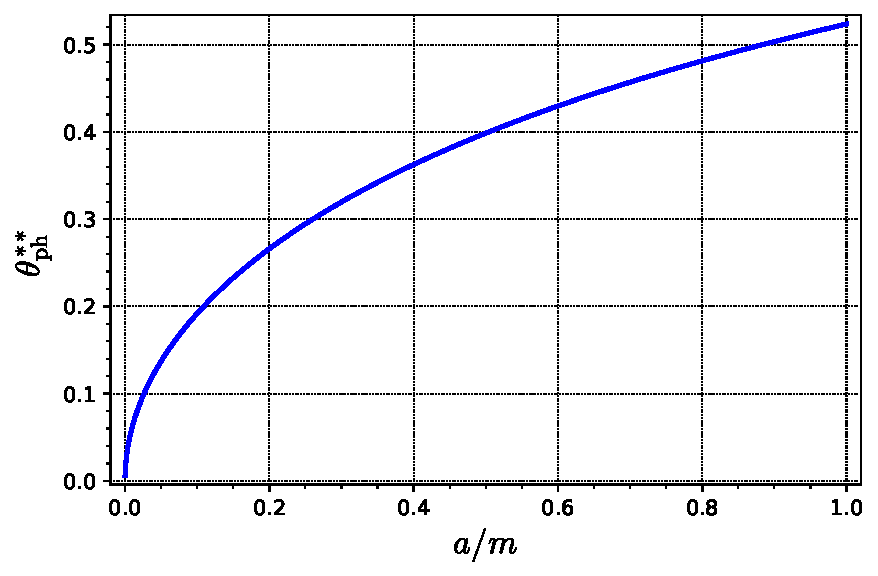
\includegraphics[width=0.6\textwidth]{gik_theta_ss.pdf}}
\caption[]{\label{f:gik:theta_ss} \footnotesize
Angle $\th$ of the Northern vortical circular photon orbit at $r = r_{\rm ph}^{**}$ as a
function of Kerr spin parameter $a$.
\textsl{[Figure generated by the notebook \ref{s:sam:Kerr_spher_photon_existence}]}
}
\end{figure}

\begin{figure}
\centerline{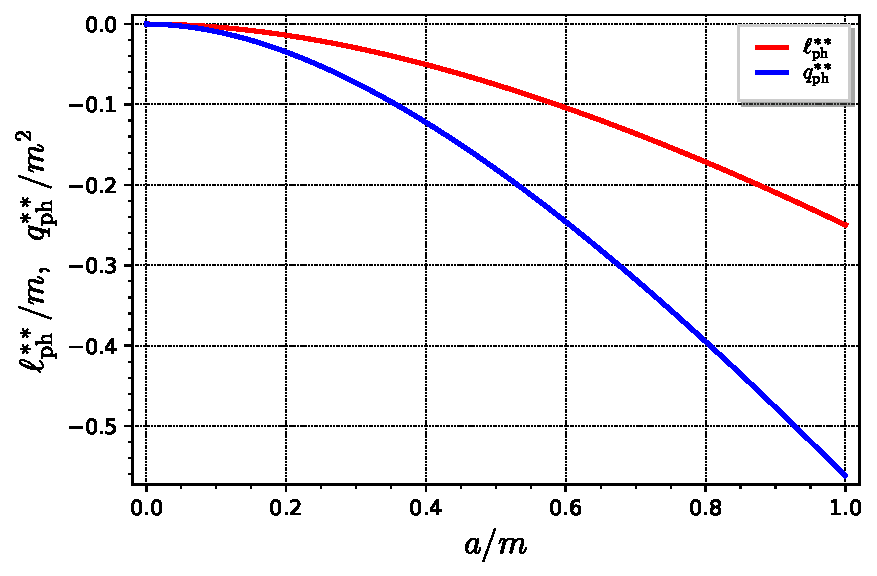
\includegraphics[width=0.6\textwidth]{gik_ell_q_rss.pdf}}
\caption[]{\label{f:gik:ell_q_rss} \footnotesize
Reduced angular momentum $\ell_{\rm ph}^{**}$ and reduced Carter constant
$q_{\rm ph}^{**}$ of the two vortical circular photon orbits
at $r = r_{\rm ph}^{**}$, as
functions of Kerr spin parameter $a$.
\textsl{[Figure generated by the notebook \ref{s:sam:Kerr_spher_photon_existence}]}
}
\end{figure}

We may summarize the above results by
\begin{greybox}
The geodesics at the boundaries of the domain of
existence of spherical photon orbits [Eq.~(\ref{e:gik:spher_orb_range})] are circular orbits:
\begin{itemize}
\item the orbit at $(r,\th)=(r_{\rm ph}^{**},\th_{\rm ph}^{**})$ is called
the \defin{Northern vortical circular photon orbit}\index{vortical!circular photon orbit}\index{circular!photon orbit!vortical --};
\item the orbit at $(r,\th)=(r_{\rm ph}^{**},\pi - \th_{\rm ph}^{**})$ is called
the \defin{Southern vortical circular photon orbit};
\item the orbit at $(r,\th)=(r_{\rm ph}^*,\pi/2)$ is called the \defin{equatorial inner circular photon orbit}\index{equatorial!circular photon orbit}\index{inner!circular!photon orbit};
\item the orbit at $(r,\th)=(r_{\rm ph}^+,\pi/2)$ is called the \defin{prograde outer circular photon orbit}\index{prograde!outer circular!photon orbit};
\item the orbit at $(r,\th)=(r_{\rm ph}^-,\pi/2)$ is called the \defin{retrograde outer circular photon orbit}\index{retrograde!outer circular!photon orbit};
\end{itemize}
Moreover, there is no other circular photon orbit with $E\neq 0$. The circular photon orbits
with $E=0$ are the null generators of the two Killing horizons $\Hor$ and $\Hor_{\rm in}$.
\end{greybox}
That the orbits listed above are the only $E\neq 0$ circular orbits follows from the fact
that all the other $E\neq 0$ spherical photon orbits have either $q > 0$ or $q_{\rm min} < q < 0$
(cf. Fig.~\ref{f:gik:spher_orb_exist}), which imply that they have a varying $\th$
(cf. Sec.~\ref{s:gik:th_motion}).

\subsection{Stability of spherical photon orbits} \label{s:gik:spher_stability}

The radial stability of spherical photon orbits is derived by the same
argument as that used in Sec.~\ref{s:gek:circ_orb_stab} for timelike circular
orbits: a spherical photon orbit at $r=r_0$ is
stable iff no geodesic motion with the same values of the
conserved quantities $\ell$ and $q$
is possible in the vicinity of $r_0$ except for $r=r_0$. Given
the same value of $(\ell,q)$ imply the same polynomial $\mathcal{R}$ and
that a geodesic
motion is possible only if $\mathcal{R}(r) \geq 0$ [Eq.~(\ref{e:mcR_non_neg})],
the above criteria is equivalent to $\mathcal{R}(r) < 0$
for $r$ distinct from $r_0$ but close to it. Since $\mathcal{R}(r_0) = 0$
and $\mathcal{R}'(r_0) = 0$ [Eq.~(\ref{e:gik:R_Rp_r0_zero})], this is equivalent
to $\mathcal{R}$ having a maximum at $r_0$. In other words:
\begin{greybox}
\be \label{e:gik:stability_spher}
    \mbox{The spherical photon orbit of radius $r_0$ is stable} \iff
    \mathcal{R}''(r_0) < 0 .
\ee
\end{greybox}
\begin{remark}
The criterion (\ref{e:gek:stability_circ_V}) for timelike circular orbits involves
$\mathcal{V}''(r_0) > 0$ simply because
of the minus sign in the definition of $\mathcal{V}$ from $R$:
$\mathcal{V}(r) := - R(r) / (\mu^2 r^4)$, whereas we have here
$\mathcal{R}(r) := R(r)/E^2$.
\end{remark}

An immediate consequence of the lemma in Sec.~\ref{s:gik:radial_motion} is
\begin{greybox}
All spherical photon orbits in the black hole exterior are unstable.
\end{greybox}
\begin{proof}
The quartic polynomial $\mathcal{R}(r)$ of spherical photon orbits in $\M_{\rm I}$
belong to case~2 of the lemma, which states that $\mathcal{R}(r)>0$ for $r\in (r_+, r_0)\cup(r_0, +\infty)$,
i.e. $r_0$ corresponds to a minimum of $\mathcal{R}$ (cf. Fig.~\ref{f:gik:R_in_M1}b).
\end{proof}

We are however going to see that there exist stable spherical photon orbits in
region $\M_{\rm III}$.
From expression~(\ref{e:gik:mcR_powers}) for $\mathcal{R}$, we get
$\mathcal{R}''(r_0) = 12 r_0^2 + 2 (a^2 - \ell^2 - q )$.
Substituting the values (\ref{e:gik:spher_ell_r0}) and (\ref{e:gik:spher_q_r0})
for respectively $\ell$ and $q$ yields
\be \label{e:gik:R_second_der}
    \mathcal{R}''(r_0) = \frac{8 r_0}{(r_0 - m)^2}
    \left[ (r_0 - m)^3 + m^3 \left( 1 - \frac{a^2}{m^2} \right) \right] .
\ee
Hence the stability criterion (\ref{e:gik:stability_spher}) becomes
\be \label{e:gik:cond_d2R_neg}
   \mathcal{R}''(r_0) < 0 \iff \begin{cases}
   r_0 < 0 \quad\mbox{and}\quad (r_0 - m)^3 + m^3 \left( 1 - \frac{a^2}{m^2} \right)  > 0 \\
   \mbox{or}\\
   r_0 > 0 \quad\mbox{and}\quad (r_0 - m)^3 + m^3 \left( 1 - \frac{a^2}{m^2} \right)  < 0 .
   \end{cases}
\ee
Now
\[
    (r_0 - m)^3 + m^3 \left( 1 - \frac{a^2}{m^2} \right)  > 0 \iff
    r_0 - m > - m \left( 1 - \frac{a^2}{m^2} \right)^{1/3}
    \iff
    r_0 > r_{\rm ph}^{\rm ms} ,
\]
where
\be \label{e:gik:r_ph_mb}
    \encadre{r_{\rm ph}^{\rm ms} := m \left[ 1 -  \left( 1 - \frac{a^2}{m^2} \right)^{1/3} \right] } .
\ee
Since obviously $r_{\rm ph}^{\rm ms} \geq 0$, we conclude that the first case in (\ref{e:gik:cond_d2R_neg})
is excluded and that the second case holds for $0 < r_0 < r_{\rm ph}^{\rm ms}$:
\begin{greybox}
\be
    \mbox{A spherical photon orbit of radius $r_0$ is stable} \iff
    0 < r_0 < r_{\rm ph}^{\rm ms}.
\ee
\end{greybox}
The index `ms' in $r_{\rm ph}^{\rm ms}$ stands for \defin{marginally stable}\index{marginally!stable spherical orbit}.
$r_{\rm ph}^{\rm ms}$ is plotted as a function of $a$ in Fig.~\ref{f:gik:spher_orb_range}.
By comparing the blue solid curve with the green dotted one in that figure,
we note that
\be
    r_{\rm ph}^{\rm ms} \leq r_{\rm ph}^* ,
\ee
with equality iff $a=m$.
We conclude
\begin{greybox}
All spherical photon orbits are unstable with respect to radial perturbations, except
for a subclass of inner orbits with negative energy\index{negative-energy particle}\index{particle!negative-energy --} ($E < 0$):
those that have a radius $r_0\in(0, r_{\rm ph}^{\rm ms})$, where $r_{\rm ph}^{\rm ms}$ is
given by Eq.~(\ref{e:gik:r_ph_mb}). In particular, all spherical photon orbits
in $\M_{\rm I}$ (the black hole exterior) are unstable, as well as all circular photon orbits
discussed in Sec.~\ref{s:gik:circular_orbits}.
\end{greybox}
That all stable orbits have $E<0$ follows from the results on the sign of $E$ obtained
in Sec.~\ref{s:gik:spher_existence}.


The stable spherical photon orbits have $q>0$ and $\ell > 0$
(cf. right panel of Fig.~\ref{f:gik:spher_orb_exist}).
According to the results of Sec.~\ref{s:gik:th_motion}, they
thus oscillate symmetrically about the equatorial plane, between
two $\th$-turning points, $\th_{\rm m}$ and $\pi-\th_{\rm m}$, such that $0<\th_{\rm m}<\pi/2$.
In particular, $r_0 = r_{\rm ms}$ does not correspond to a unique orbit, but
to a 1-parameter family of marginally stable orbits; the parameter can be chosen
to be the azimuthal coordinate $\ph$ at the first value $\th=\th_{\rm m}$ (or $\th=\pi/2$)
after $t=0$. A marginally stable spherical photon orbit is
shown in Fig.~\ref{f:gik:spher_3d_ms}.

We have the following property, which appears clearly on Fig.~\ref{f:gik:spher_orb_exist}:
\begin{greybox}
Among all inner spherical photon orbits, the marginally stable orbits
at $r_0 = r_{\rm ph}^{\rm ms}$ are those for which the reduced angular momentum $\ell$
and reduced Carter constant $q$ are maximal.
\end{greybox}
\begin{proof}
From Eqs.~(\ref{e:gik:spher_ell_r0}) and (\ref{e:gik:spher_q_r0}), we get
\be \label{e:gik:spher_orb_dqdr}
   \derd{q_{\rm c}}{r_0} = - \frac{4 r_0^2 (r_0 - 3m) \left[ (r_0 - m)^3 + m^3 \left(1 - \frac{a^2}{m^2}
            \right)\right]}{a^2 (r_0 - m)^3}
\ee
\be
   \derd{\ell_{\rm c}}{r_0} = - 2 \frac{(r_0 - m)^3 + m^3 \left(1 - \frac{a^2}{m^2}
            \right)}{a (r_0 - m)^2}
\ee
Since $r_{\rm ph}^{\rm ms}$ is the unique real root of
$(r_0 - m)^3 + m^3 (1 - a^2/m^2) = 0$ [cf. Eq.~(\ref{e:gik:R_second_der})],
it is clear that the function $\ell_{\rm c}(r_0)$ has a unique extremum, which is
achieved by the marginally stable orbits. From the graph of $\ell_{\rm c}(r_0)$
shown in Fig.~\ref{f:gik:spher_orb_exist}, we see that this extremum is
a maximum. Regarding the function $q_{\rm c}(r_0)$, the above expression of $\D q_{\rm c}/\D r_0$
leads to two extrema: $r_0 = r_{\rm ph}^{\rm ms}$ and $r_0 = 3 m$.
The former regards the inner spherical orbits, while the latter regards
the outer ones. Again, from the graph shown in Fig.~\ref{f:gik:spher_orb_exist},
it is clear that $r_0 = r_{\rm ph}^{\rm ms}$ realizes a maximum of $q_{\rm c}$
among all inner spherical orbits.
\end{proof}

\begin{remark}
Another proof can be given by using the same general argument as that employed in
Sec.~\ref{s:gek:circ_orb_stab} (p.~\pageref{p:gek:ISCO_extremum_eps_ell})
for showing that the ISCO realizes an extremum of the specific energy
and specific angular momentum of timelike circular equatorial orbits.
Indeed, considering $\mathcal{R}$ as a function of $\ell$ and $q$, in addition
to $r$, i.e. writing $\mathcal{R} = \mathcal{R}(r, \ell, q)$, the marginal
stable orbit obeys
\[
    \mathcal{R}(r_0, \ell_{\rm c}(r_0), q_{\rm c}(r_0)) = 0,\quad
    \der{\mathcal{R}}{r}(r_0, \ell_{\rm c}(r_0), q_{\rm c}(r_0)) = 0,\quad
    \frac{\partial^2\mathcal{R}}{\partial r^2} (r_0, \ell_{\rm c}(r_0), q_{\rm c}(r_0)) = 0 .
\]
Deriving the first and second equations with respect to $r_0$
and using the third equation, we get a homogeneous linear
system for $(\D\ell_{\rm c}/\D r_0,\, \D q_{\rm c}/\D r_0)$, similar to the
system (\ref{e:gek:system_epsp_ellp}). The unique solution
is then $(\D\ell_{\rm c}/\D r_0,\, \D q_{\rm c}/\D r_0) = (0, 0)$, yielding the extremum in the
functions $\ell_{\rm c}(r_0)$ and $q_{\rm c}(r_0)$ at $r_0 = r_{\rm ph}^{\rm ms}$.
\end{remark}

Equation~(\ref{e:gik:spher_orb_dqdr}) shows that, in addition to that
at $r_0 = r_{\rm ph}^{\rm ms}$, the function $q_{\rm c}(r_0)$ admits
a second extremum at $r_0 = 3m$, i.e. for outer spherical orbits.
This extremum is actually a maximum and its value, obtained by
setting $r_0 = 3 m$ in Eq.~(\ref{e:gik:spher_q_r0}),
turns out to be independent from $a$:
\be \label{e:gik:spher_max_q}
    \max q_{\rm c}(r_0) = 27 m^2 .
\ee
This is the maximum of the reduced Carter constant over all the spherical photon
orbits (cf. Fig.~\ref{f:gik:spher_orb_exist}).


\begin{figure}
\parbox[c]{0.49\textwidth}{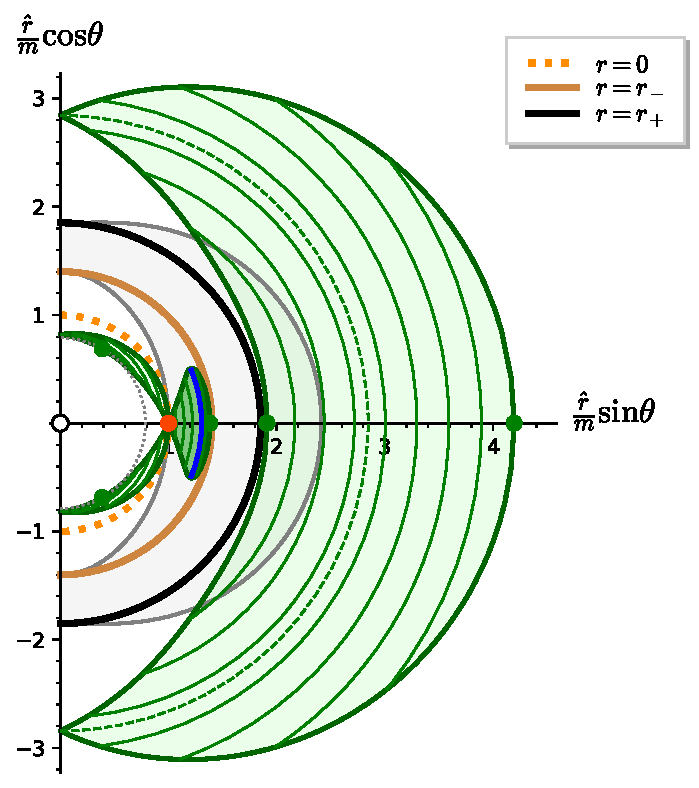
\includegraphics[width=0.49\textwidth]{gik_spo_meridional.pdf}}
\parbox[c]{0.49\textwidth}{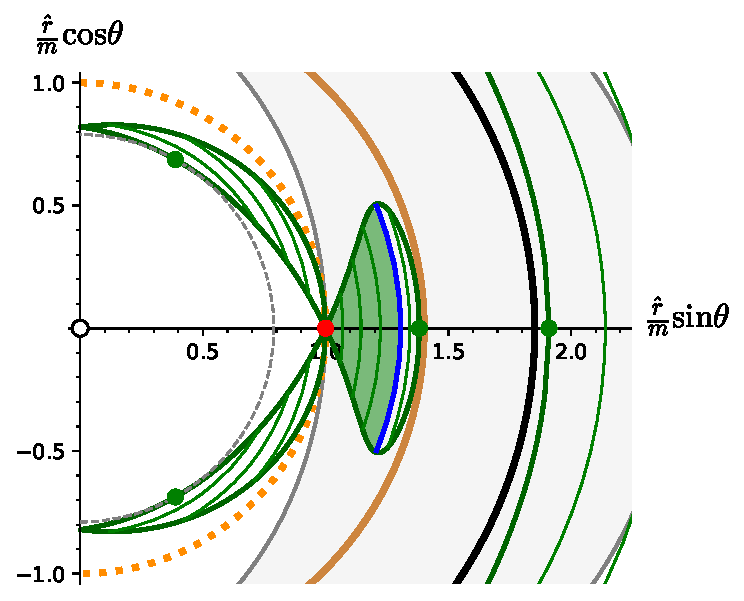
\includegraphics[width=0.49\textwidth]{gik_spo_meridional_zoom.pdf}}
\caption[]{\label{f:gik:spo_meridional} \footnotesize
Trace of the photon region (pale and dark green areas) in
a meridional plane $(t,\ph)=\mathrm{const}$ of
a Kerr spacetime with $a = 0.95\, m$ (as in Fig.~\ref{f:gik:spher_orb_exist}).
The right panel is a zoom on the inner part of the left one.
The meridional plane is described in terms of the coordinates $(\hat{r},\th)$
where $\hat{r} := (r + \sqrt{r^2 + 4m^2})/2$ [cf. Eq.~(\ref{e:gik:def_hat_coord})].
Some spherical photon orbits are shown as green circular arcs,
with the dashed ones representing the polar spherical orbits, i.e. $\ell=0$ orbits.
The black (resp. light brown) half-circle at $r=r_+$ (resp. $r=r_-$)
is the trace of the outer (resp. inner) Killing horizon.
The dotted orange half-circle marks the locus of $r=0$, with the
red dot indicating the curvature singularity at $r=0$ and $\th=\pi/2$.
The ergoregion is shown in grey. The region of stable spherical orbits is
colored in dark green, with its boundary at $r=r_{\rm ph}^{\rm ms}$ drawn in blue.
Green dots marks photon circular orbits: from the left to the right, they
are the two vortical circular orbits at $r=r_{\rm ph}^{**}$, the equatorial
inner circular orbit at $r=r_{\rm ph}^*$, the prograde outer circular orbit
at $r=r_{\rm ph}^+$ and the retrograde outer circular orbit at $r=r_{\rm ph}^-$.
The thin dotted grey half-circle marks $r=r_{\rm ph}^{**}$.
\textsl{[Figure generated by the notebook \ref{s:sam:Kerr_spher_photon_existence}]}
}
\end{figure}


\subsection{Photon region} \label{s:gik:photon_region}

A corollary of the results obtained in Sec.~\ref{s:gik:radial_motion}
is that outside the black hole, i.e. in region $\M_{\rm I}$, a photon
cannot be trapped (i.e. move in a limited range of $r$) unless it moves
on a (unstable) spherical orbit. The part of Kerr spacetime made of points
through which a spherical photon orbit can pass is called the
\defin{photon region}\index{photon!region} or sometimes the \defin{photon shell}\index{photon!shell} \cite{Johns_al20}. In terms of the Boyer-Lindquist $r$-coordinate, the photon region
lies in the three intervals (\ref{e:gik:spher_orb_range}).
The range of the $\th$-coordinate has been discussed in Sec.~\ref{s:gik:spher_latitudinal}:
spherical photon orbits with $r_0 > 0$ oscillate about the equatorial plane
with the limiting angle $\th_{\rm m}$ given by Eq.~(\ref{e:gik:th0}) ($\th_{\rm m}=\pi/2$
for the three circular orbits at $r_0 = r_{\rm ph}^*$, $r_0=r_{\rm ph}^+$
and $r_0 = r_{\rm ph}^-$, which lie in the equatorial plane). On the other side,
the inner orbits with $r_0 < 0$ are all vortical, with the limiting
angles $\th_{\rm m}$ and $\th_{\rm v}$ given by Eqs.~(\ref{e:gik:th0}) and (\ref{e:gik:th1_general}).
There is no constraint on the Boyer-Lindquist $\ph$-coordinate: the photon region occupies
all the range $[0, 2\pi)$.

The photon region is depicted in Fig.~\ref{f:gik:spo_meridional}, which represents
a meridional plane $(t,\ph) = \mathrm{const}$ of a Kerr spacetime with $a=0.95\, m$
--- the same value of $a$ as in Fig.~\ref{f:gik:spher_orb_exist}.
Polar spherical photon orbits, at $r_0 = r_{\rm ph}^{\rm pol}$ and $r_0 = r_{\rm ph}^{\rm pol,in}$
(cf. Sec.~\ref{s:gik:spher_latitudinal}), are plotted as dashed green curves.
It is graphically clear that they are the only orbits that encounter the rotation axis.
We also recover from this figure that, apart from those generating the two horizons $\Hor_{\rm in}$
and $\Hor$, the only circular photon orbits of Kerr spacetime are the
five ones considered in Sec.~\ref{s:gik:circular_orbits} (the five green dots).
We note also that a part of the outer spherical photon orbits lie in the ergoregion. These orbits
have however $E>0$, according to the results of the end of Sec.~\ref{s:gik:spher_existence}.

\begin{hist}
The prograde and retrograde outer circular photon orbits in the equatorial plane
of a Kerr black hole have been found by James M. Bardeen\index{Bardeen, J.M.}, William H. Press\index{Press, W.H.} and Saul A. Teukolsky\index{Teukolsky, S.A.} in 1972 \cite{BardePT72}.
The existence of stable spherical photon orbits under the inner horizon
of a Kerr black hole has been shown by Zden\v{e}k Stuchl\'{\i}k\index{Stuchl\'{\i}k, Z.}
in 1981 \cite{Stuch81}. The systematic study of spherical photon orbits
in the black hole exterior has been performed by Edward Teo\index{Teo, E.} in 2003 \cite{Teo03}.
\end{hist}


%%%%%%%%%%%%%%%%%%%%%%%%%%%%%%%%%%%%%%%%%%%%%%%%%%%%%%%%%%%%%%%%%%%%%%%%%%%%%%%

\section{Black hole shadow and critical curve} \label{s:gik:shadow}

\subsection{Critical null geodesics} \label{s:gik:critical_geod}

As in the Schwarzschild case (Sec.~\ref{s:gis:crit_geod}), let us define
a \defin{critical null geodesic}\index{critical!null geodesic!in Kerr spacetime}
as a null geodesic with $E\neq 0$ that has the same constants of motion
$(\ell,q)$ as a spherical photon orbit, but that does not stay at a fixed value
of $r$. Equivalently, a critical null geodesic
is a null geodesic with varying $r$ and for which the quartic polynomial $\mathcal{R}(r)$
[Eq.~(\ref{e:gik:mcR})] admits a double root [Eq.~(\ref{e:gik:R_Rp_r0_zero})].

In Schwarzschild spacetime (Chap.~\ref{s:gis}),
a critical null geodesic was simply any null geodesic with varying $r$
that has $b = |\ell| = 3\sqrt{3}\, m$.
In the Kerr case with $0 < a < m$, we have instead a 1-parameter family of critical values:
the family $(\ell_{\rm c}(r_0),q_{\rm c}(r_0))$ given by Eqs.~(\ref{e:gik:spher_ell_r0})--(\ref{e:gik:spher_q_r0}), the
parameter being $r_0$. By construction, the polynomial $\mathcal{R}(r)$
of a critical null geodesic $\Li$ of parameter\footnote{The word \emph{parameter} is
used here for the index among the family of all null critical geodesics and shall
not be confused with the \emph{affine parameter} along $\Li$.} $r_0$ has a double root at $r=r_0$
[cf. Eq.~(\ref{e:gik:R_Rp_r0_zero})]. More precisely, inserting formula
(\ref{e:gik:spher_ell_r0}) for $\ell$ and formula~(\ref{e:gik:spher_tq_r0})
for $\tilde{q} := q + (\ell - a)^2$
into expression (\ref{e:gik:mcR_Delta}) for $\mathcal{R}(r)$ leads to
\be \label{e:gik:mR_critical_null}
    \mathcal{R}(r) = (r - r_0)^2 \left( r^2 + 2 r_0 r - \frac{a^2 q_{\rm c}(r_0)}{r_0^2} \right) ,
\ee
where $q_{\rm c}(r_0)$ is the function (\ref{e:gik:spher_q_r0}).
This writing of $\mathcal{R}(r)$ clearly exhibits the double root at $r=r_0$.
As discussed in Sec.~\ref{s:gek:asymptotic_values} and \ref{s:gik:radial_motion},
a consequence of the double-root behavior is that
any critical null geodesic $\Li$ of paramater $r_0$ has
$r_0$ as an asymptotic $r$-value, i.e. $r(\lambda)\to r_0$
when $\lambda\to+\infty$ or $\lambda\to-\infty$, where $\lambda$ is the affine
parameter along $\Li$.

Let us consider a critical null geodesic $\Li$ of parameter $r_0$
that goes through a point $A$ of Boyer-Lindquist coordinates
$(t_A, r_A, \th_A, \ph_A)$.
By plugging (\ref{e:gik:mR_critical_null}) into the integrated equation
of motion (\ref{e:gek:integr_Mino}), we get, at any point of coordinates
$(t,r,\th,\ph)$ along $\Li$,
\be \label{e:gik:div_int_r_crit}
    \dashint_{r_A}^r \frac{\eps_r \, \D \bar{r}}{|\bar{r}-r_0|\sqrt{\bar{r}^2 + 2r_0 \bar{r} - a^2 q_{\rm c}(r_0)/r_0^2}}
   = \dashint_{\th_A}^\th
   \frac{\eps_\th \, \D \bar{\th}}{\sqrt{\tilde{\Theta}(\bar{\th})}} .
\ee
When $r\to r_0$, it is clear that the integral in the left-hand side diverges
logarithmically in terms of $|r - r_0|$.
The path integral in the right-hand side must therefore diverge as well,
which implies that $\Li$ has an endless oscillatory $\th$-motion as $r\to r_0$.
Similarly the integrated equation of motion (\ref{e:gek:integr_ph})
with expression (\ref{e:gik:mR_critical_null}) for $\mathcal{R}(r)$
becomes
\be \label{e:gik:div_phi_crit}
    \ph - \ph_{\rm em} = a \dashint_{r_A}^r
    \frac{(2m\bar{r}- a \ell) \, \eps_r \, \D \bar{r}}%
    {|\bar{r}-r_0|(\bar{r}^2 - 2m \bar{r} + a^2)\sqrt{\bar{r}^2 + 2r_0 \bar{r} - a^2 q_{\rm c}(r_0)/r_0^2}}
    + \ell \dashint_{\th_A}^\th \frac{\eps_\th \, \D \bar{\th}}{\sin^2\bar{\th}
    \sqrt{\tilde{\Theta}(\bar{\th})}} .
\ee
Again, the first integral diverges when $r\to r_0$. The second one, which is
a path integral on $\th$, diverges as well because the path integral in the
right-hand side of Eq.~(\ref{e:gik:div_int_r_crit}) diverges. From
expression (\ref{e:gik:spher_ell_r0}) for $\ell$ it can be checked
that $2 m r_0 - a \ell > 0$ in the allowed range of $r_0$ (i.e. in the
range (\ref{e:gik:spher_orb_range}),
where spherical orbits exist). Given that $\epsilon_r \, \D \bar{r} > 0$
and $\eps_\th \, \D \bar{\th} > 0$, we conclude that the integral on $r$
and the path integral on $\th$ both tend to $+\infty$ when $r\to r_0$.
If $\ell \geq 0$, we get then immediately $\ph \to + \infty$ when $r \to r_0$.
If $\ell < 0$, the two diverging terms in the right-hand side of Eq.~(\ref{e:gik:div_phi_crit})
have opposite signs.
Disregarding some unexpected subtle compensation, one term (in practice the second one) dominates
over the other one, so that we conclude that, whatever the sign of $\ell$,
\be
    \ph \to \pm \infty \quad\mbox{when}\quad r\to r_0 .
\ee

\begin{figure}
\centerline{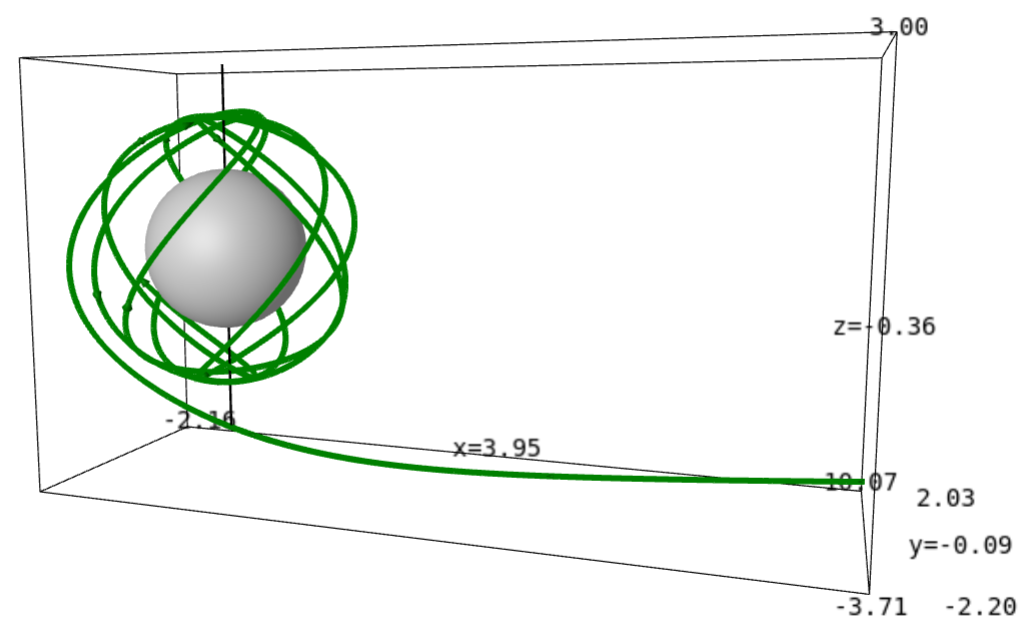
\includegraphics[width=0.7\textwidth]{gik_critical_geod.png}}
\caption[]{\label{f:gik:gik_critical_geod} \footnotesize
Critical null geodesic of parameter $r_0=2.2\, m$ in a Kerr spacetime
with $a=0.95\, m$, depicted in terms of the  Cartesian Boyer-Lindquist coordinates
$(x,y,z)$ [Eq.~(\ref{e:gek:Cartesian_BL})]. This geodesic has $\ell = 0.863\, m$,
$q = 18.042\, m^2$ and is emitted at $\lambda=0$
from the point of Boyer-Lindquist coordinates $(r,\th,\ph) = (40\, m, \pi/2, 0)$
$\iff$ $(x,y,z) = (40\, m, 0, 0)$,
towards the black hole ($\eps_r = -1$). The drawing is interrupted at
$\lambda=80\, m/E$. The grey sphere is the black hole event horizon at
$r = r_+ = 1.312\, m$.
\textsl{[Figure generated by the notebook \ref{s:sam:Kerr_null_geod_plots}]}
}
\end{figure}

We may summarize the above results as follows.
\begin{greybox}
A critical null geodesic $\Li$ of parameter $r_0$ has $r_0$ as an asymptotic $r$-value,
either in the future ($r(\lambda) \to r_0$ when $\lambda\to +\infty$) or in the
past ($r(\lambda) \to r_0$ when $\lambda\to -\infty$), $\lambda$ being the (future-directed) affine
parameter of $\Li$. In particular, $\Li$ never crosses the sphere $r=r_0$.
Moreover $\Li$ is winding endlessly on the sphere $r=r_0$ when
either $\lambda\to+\infty$ or $\lambda\to-\infty$, mimicking there the behavior of
a spherical photon orbit.
\end{greybox}



\begin{example} \label{x:gik:critical_geod}
Figure~\ref{f:gik:gik_critical_geod} shows a critical null geodesic
emitted from the equatorial plane at a large distance from the black hole
(the emission point is not shown on the figure that is truncated
at $r\sim 10\, m$). We note the winding around the sphere $r=r_0 = 2.2\, m$,
in the same fashion as a spherical photon orbit (compare with Figs.~\ref{f:gik:spher_3d_r_16}
and \ref{f:gik:spher_3d_r_28}).
\end{example}

\begin{figure}
\centerline{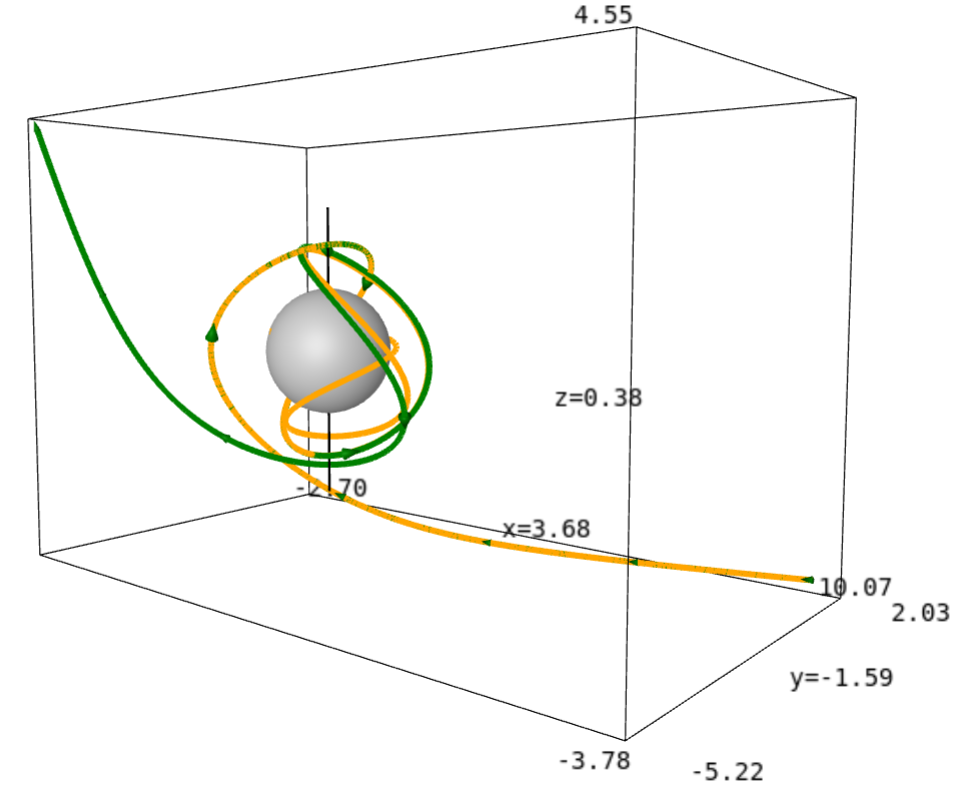
\includegraphics[width=0.6\textwidth]{gik_close_critical.png}}
\caption[]{\label{f:gik:close_critical} \footnotesize
Two null geodesics with constants of motion $(\ell,q)$ close
to those of a critical null
geodesic, $(\ell_{\rm c}(r_0),q_{\rm c}(r_0))$
[Eqs.~(\ref{e:gik:spher_ell_r0})--(\ref{e:gik:spher_q_r0})]. Here,
as in Fig.~\ref{f:gik:gik_critical_geod}, $r_0=2.2\, m$ and $a=0.95\, m$.
The two geodesics depart from the
same point at $(x,y,z)=(40\, m, 0, 0)$ (outside the scope of the figure)
as the critical null geodesic shown in Fig.~\ref{f:gik:gik_critical_geod}.
Both geodesics have $q = q_{\rm c}(r_0)$, but the green one
has $\ell = 1.0001\,\ell_{\rm c}(r_0)$
while the orange one has $\ell = 0.9999\,\ell_{\rm c}(r_0)$.
\textsl{[Figure generated by the notebook \ref{s:sam:Kerr_null_geod_plots}]}
}
\end{figure}



\subsection{Critical curve and black hole shadow} \label{s:gik:shadow_generic}

In this section, we focus on null geodesics emitted in the black hole
exterior, i.e. in region $\M_{\rm I}$, having in mind the formation
of images on the screen of a distant observer.
As in the Schwarzschild case studied in Chap.~\ref{s:gis}, the family
of critical null geodesics separates the null geodesics emitted far from the
black hole between those
that can escape to infinity and those that fall into the black hole.
More precisely, according to the lemma established in Sec.~\ref{s:gik:radial_motion},
this family separates null geodesics whose quartic polynomial $\mathscr{R}$
has no root in $\M_{\rm I}$ from those for which $\mathscr{R}$ has a double
root in $\M_{\rm I}$. It follows that the family of critical null
geodesics separates null geodesics that have a $r$-turning
point in $\M_{\rm I}$ from those that do not have any, given that a null geodesic has at most
one $r$-turning point in $\M_{\rm I}$ (cf. Sec.~\ref{s:gik:radial_motion}).
This is illustrated by the following example.

\begin{example}
Figure~\ref{f:gik:close_critical} depicts
two null geodesics initially very close to a critical one.
They are emitted at the same point as the critical geodesic considered in Example~\ref{x:gik:critical_geod}
and with parameters close to critical: the same reduced Carter constant $q$
and values of the reduced angular momentum $\ell$ almost equal to the critical
one, $\ell_{\rm c}(r_0)$, up to a relative difference of $10^{-4}$.
The geodesic $\Li_1$ (green curve) has $\ell = 1.0001\,\ell_{\rm c}(r_0)$; it performs a few
turns onto (actually very close to) the sphere $\Sp_0$ of coordinate radius $r_0 = 2.2\, m$ and eventually depart to infinity; this means that $\Li_1$ has a $r$-turning point, somewhere close
to $\Sp_0$.
The geodesic $\Li_2$ (orange curve) has $\ell = 0.9999\,\ell_{\rm c}(r_0)$; it is
graphically undistinguishable from $\Li_1$ until a full turn onto $\Sp_0$
(this is best seen in the interactive 3D view in the online notebook \ref{s:sam:Kerr_null_geod_plots}),
it then clearly
departs from it and eventually terminates into the black hole. Hence $\Li_2$ has no $r$-turning
point.
\end{example}

Let us consider an asymptotic inertial observer $\Obs$ (cf. Sec.~\ref{s:ker:asymp_inertial_obs}),
i.e. a static observer located at Boyer-Lindquist coordinates $(t,r_{\Obs},\th_{\Obs},\ph_{\Obs})$,
where $(r_{\Obs},\th_{\Obs},\ph_{\Obs})$ are constant and $r_{\Obs} \gg m$.
As in the Schwarzschild case (Sec.~\ref{s:gis:shadow}), the concept of
black hole shadow is defined by considering an emitting large sphere $\Sp$
of constant Boyer-Lindquist coordinate $r_{\Sp}$ that
encompasses both the black hole and observer $\Obs$; this means that
$r_{\Sp} > r_{\Obs}$. In a more astrophysical setting, one could image $\Sp$
as being made of many far-away light sources.
We assume that $\Obs$ is equipped with a screen in the
direction of the black hole, in the same set up as described in Sec.~\ref{s:gik:remote_screen}
(cf. Fig.~\ref{f:gik:obs_screen}). Given the relative position of $\Obs$, the black hole
and the emitting sphere $\Sp$, any photon emitted from $\Sp$ that reaches $\Obs$'s screen
has necessarily a point of minimal approach to the black hole, i.e. the associated
null geodesic has necessarily a $r$-turning point between $\Sp$ and $\Obs$.
Reciprocally, any null geodesic that impacts $\Obs$'s screen and has no
$r$-turning point in its past cannot have emerged from $\Sp$ and therefore
results in a black dot on the screen. According to the above discussion, the
boundary of the black area on $\Obs$'s screen is made by the impact points of
critical null geodesics and is called the \defin{critical curve}\index{critical!curve}
\cite{GrallHW19,GrallL20a}; we shall denote it by $\mathscr{C}$.
The black area itself is called the
\defin{black hole shadow}\index{black hole!shadow}\index{shadow!black hole --}.
It is called so essentially because if the black hole were not present, it would
not exist and $\Obs$'s screen would be uniformly bright.

\begin{remark}
The concept of black hole shadow is rather academic, since it
requires the sources of light to be far from the black hole and to surround it, as well
as the observer, from any direction. On the contrary, astrophysical black holes
are illuminated by close sources (e.g. an accretion disk) and we shall see in Sec.~\ref{s:gik:images}
that the black area on astronomical images has little ressemblance with the shadow defined above.
On the other hand, the critical curve has a true observational significance, as we shall discuss
in Sec.~\ref{s:gik:images}, and is definitely worth to study.
\end{remark}

In what follows, we shall assume that the observer $\Obs$ in not located
on the black hole rotation axis, i.e. $\th_{\Obs}\not\in\{0, \pi\}$,
leaving the special case $\th_{\Obs} = 0$ or $\pi$ to Sec.~\ref{s:gik:shadow_rot_axis}.
Then $\sin\th_{\Obs}\neq 0$ and we have seen in Sec.~\ref{s:gik:remote_screen} that
the impact point of a null geodesic $\Li$ on $\Obs$'s screen, measured by
the screen angular coordinates\index{screen!angular coordinates}\index{angular!screen -- coordinates}
$(\alpha,\beta)$,
is related to the reduced angular momentum $\ell$
and reduced Carter constant $q$ of $\Li$ by formulas
(\ref{e:gik:screen_alpha_beta}).
Given the above definition, the critical curve $\mathscr{C}$ is obtained by
using for $(\ell,q)$ in (\ref{e:gik:screen_alpha_beta})
the critical values $(\ell_{\rm c}(r_0),q_{\rm c}(r_0))$
given by Eqs.~(\ref{e:gik:spher_ell_r0})--(\ref{e:gik:spher_q_r0}):
\begin{subequations}
\label{e:gik:shadow_param_eq}
\begin{align}
& \alpha =  - \frac{\ell_{\rm c}(r_0)}{r_{\Obs}\sin\th_{\Obs}}  \label{e:gik:shadow_param_eq_alpha}\\
& \beta =  \frac{\eps_\th}{r_{\Obs}}
        \sqrt{ q_{\rm c}(r_0) + \cos^2\th_{\Obs} \left( a^2
    - \frac{\ell_{\rm c}(r_0)^2}{\sin^2\th_{\Obs}} \right) } . \label{e:gik:shadow_param_eq_beta}
\end{align}
\end{subequations}
This provides the equation of $\mathscr{C}$ in parametric form,
the parameter being $r_0$ --- the radius of the spherical orbits that have
the same value of $(\ell, q)$ as the critical null geodesic that impacts
$\Obs$'s screen at the point $(\alpha,\beta)$.
Let us recall that $(\alpha,\beta)$ are angular coordinates and are therefore dimensionless
(cf. Sec.~\ref{s:gik:remote_screen}).
The range of $r_0$ for spherical orbits in the black hole exterior
is $r_{\rm ph}^+ \leq r_0 \leq r_{\rm ph}^-$ [Eq.~(\ref{e:gik:spher_orb_range})],
with $r_{\rm ph}^+$ and $r_{\rm ph}^-$ given by Eq.~(\ref{e:gik:rph_pm}). The corresponding
range of $\ell=\ell_{\rm c}(r_0)$ is then
$\ell_{\rm c}(r_{\rm ph}^-) \leq \ell \leq  \ell_{\rm c}(r_{\rm ph}^+)$
(cf. the red curve in Fig.~\ref{f:gik:spher_orb_exist}) and the
corresponding range of $q = q_{\rm c}(r_0)$ is
$0 \leq q \leq 27\, m^2$ [cf. Eq.~(\ref{e:gik:spher_max_q})].
However, not all these values of $(\ell, q)$ are allowed, since in
order for the corresponding geodesic to reach $\Obs$, they have to obey the
constraint (\ref{e:gik:constraint_theta_obs}):
\be \label{e:gik:constraint_theta_obs_r0}
  \left( q_{\rm c}(r_0) + a^2 \cos^2\th_{\Obs} \right) \sin^2\th_{\Obs}
         - \ell_{\rm c}(r_0)^2 \cos^2\th_{\Obs} \geq 0 .
\ee
Except for $\th_{\Obs} = \pi/2$ (observer in the equatorial plane), this constraint
limits the range of $r_0$ to a subinterval $[r_0^{\rm min}, r_0^{\rm max}]$
of $[r_{\rm ph}^+, r_{\rm ph}^-]$. We note that the radius
$r_{\rm ph}^{\rm pol}$ of polar spherical photon orbits, as given by
Eq.~(\ref{e:gik:rph_pol}), lies necessarily in that subinterval;
indeed by definition $\ell_{\rm c}(r_{\rm ph}^{\rm pol}) = 0$, which ensures that
the constraint (\ref{e:gik:constraint_theta_obs_r0}) is fulfilled for
$r_0 = r_{\rm ph}^{\rm pol}$, whatever the value of $\th_\Obs$.

\begin{figure}
\begin{center}
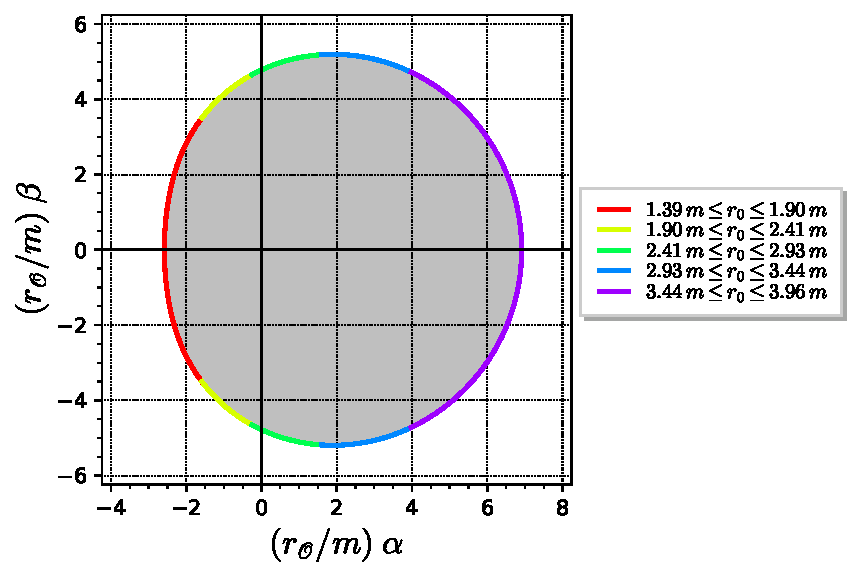
\includegraphics[height=0.28\textheight]{gik_shadow_a95_th90.pdf} \\[1ex]
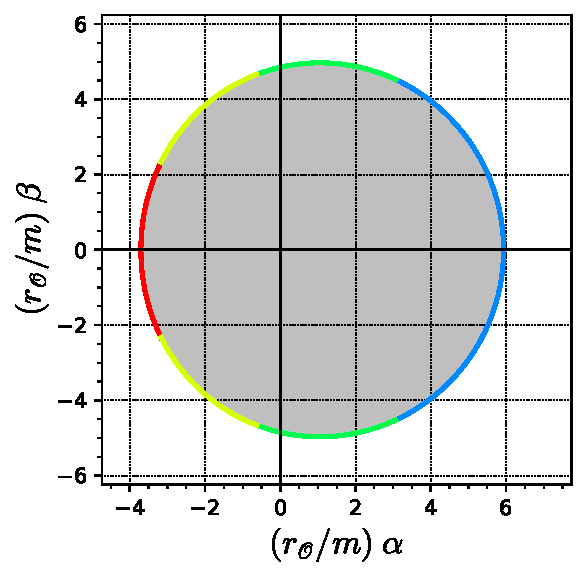
\includegraphics[height=0.28\textheight]{gik_shadow_a95_th30.pdf}\qquad
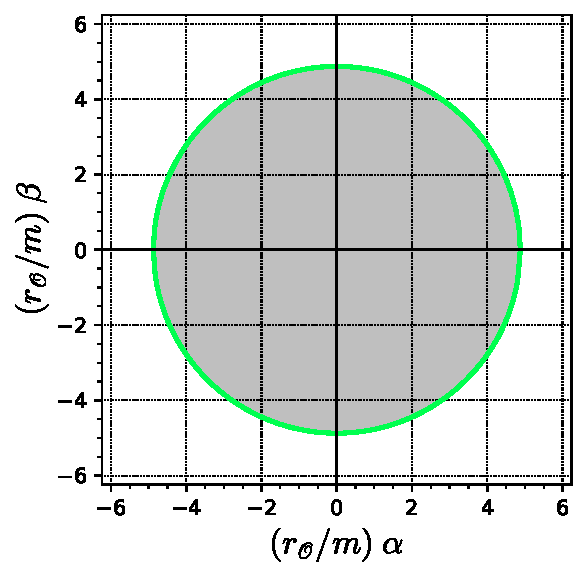
\includegraphics[height=0.28\textheight]{gik_shadow_a95_th00.pdf}
\end{center}
\caption[]{\label{f:gik:shadow_a95} \footnotesize
Shadow of a Kerr black hole of mass $m$ and spin parameter $a=0.95\, m$ on the screen of an asymptotic
inertial observer $\Obs$ located at $r=r_{\Obs}$ and $\th=\th_{\Obs}$, for three
values of $\th_{\Obs}$: $\th_{\Obs} = \pi/2$ ($\Obs$ in the equatorial plane; upper panel),
$\th_{\Obs} = \pi/6$ (lower left) and $\th_{\Obs} = 0$ ($\Obs$ on the rotation axis; lower right).
The screen is spanned by the angular coordinates $(\alpha,\beta)$, rescaled by the inverse of
the factor $m/r_{\Obs}$, whose values for some astrophysical black holes can be found in Table~\ref{t:gik:scale_factor}.
The shadow is bounded by the critical curve $\mathscr{C}$, which is depicted
with colors indicating the range of the parameter $r_0$
of the critical null geodesics forming it.
\textsl{[Figure generated by the notebook \ref{s:sam:Kerr_shadow}]}
}
\end{figure}

\begin{table}
\centerline{
\begin{tabular}{|l|c|c|c|c|}
\hline
 & Sgr A* & M87* & M31* & Cyg X-1 \\[0.5ex]
\hline\hline
$m$ [$M_\odot$] & $4.1 \; 10^6$ & $6.2\; 10^9$ & $1.5\; 10^8$ & $15$ \\[0.5ex]
\hline
$r_{\Obs}$ [kpc] & $8.12$ & $1.67\; 10^4$ & $7.6\; 10^2$ & $1.86$ \\[0.5ex]
\hline
$m/r_{\Obs}$ & $2.4\; 10^{-11}$ & $1.8\; 10^{-11}$ & $9.4\; 10^{-12}$ & $3.9\; 10^{-16}$ \\[0.5ex]
\hline
$m/r_{\Obs}$ [$\mu$as] & $5.0$ & $3.7$ & $1.9$ & $8.0\; 10^{-5}$ \\[0.5ex]
\hline
\end{tabular}
}
\caption[]{\label{t:gik:scale_factor} \footnotesize
Scale factor $m/r_{\Obs}$ for various astrophysical black holes:
the supermassive black hole at the center of our galaxy,
Sagittarius A*\index{Sagittarius A*} (data taken from Table~A.1 of Ref.~\cite{Abute_al18a}), the supermassive black hole M87*\index{M87*} in the nucleus of the galaxy
Messier~87 (data from Refs.~\cite{Gebha_al11,EHT19a}), the supermassive black hole M31*
in the nucleus of the Andromeda Galaxy (Messier~31) (data from Ref.~\cite{Bende_al05})
and the stellar black hole Cygnus X-1\index{Cygnus X-1}
(data from Refs.~\cite{Orosz_al11,Reid_al11,Gou_al14}). The last line gives $m/r_{\Obs}$
in microarcseconds ($1\; \mu{\rm as} = 4.848\; 10^{-12}\; {\rm rad}$).
}
\end{table}



The critical curve $\mathscr{C}$ in the observer's screen is obtained by first solving
Eq.~(\ref{e:gik:constraint_theta_obs_r0}) with equality in the sign $\geq$
to determine $r_0^{\rm min}$ and  $r_0^{\rm max}$. Then, the upper half of
$\mathscr{C}$ is computed by means of formulas~(\ref{e:gik:shadow_param_eq})
with $\eps_\th=+1$ and $r_0$ ranging in $[r_0^{\rm min}, r_0^{\rm max}]$.
The lower half is obtained similarly, but with $\eps_\th = -1$ in Eq.~(\ref{e:gik:shadow_param_eq_beta}),
so that it is the symmetric of the upper half with respect to the $\alpha$-axis.

The result of the computation is shown in
Fig.~\ref{f:gik:shadow_a95} for a Kerr black hole with
$a=0.95\, m$ and various inclination angles of observer $\Obs$.
For $\th_{\Obs}=\pi/2$ the parameter $r_0$ of the critical null geodesics
forming $\mathscr{C}$ spans the full interval
$[r_{\rm ph}^+, r_{\rm ph}^-] \simeq [1.386\, m,\; 3.955\, m]$.
For $\th_{\Obs}=\pi/6$, the range is restricted to
$[r_0^{\rm min}, r_0^{\rm max}] \simeq [1.768\, m,\;   3.237\, m]$,
while for $\th_{\Obs}=0$ (to be discussed in Sec.~\ref{s:gik:shadow_rot_axis}),
$r_0$ can take only one value:
$r_0 = r_{\rm ph}^{\rm pol} \simeq 2.493\, m$.
At a fixed value of $a/m$, the black hole shadow depends on $m$ and $r_{\Obs}$
only through the dimensionless ratio $m/r_{\Obs}$, which sets the global scale of the shadow.
Accordingly, in Fig.~\ref{f:gik:shadow_a95}, the screen angular coordinates $(\alpha,\beta)$ have
been rescaled by $(m/r_{\Obs})^{-1}$.
Values of $m/r_{\Obs}$ for some astrophysical black holes are provided
in Table~\ref{t:gik:scale_factor}; the observer's radial coordinate $r_{\Obs}$ is then
nothing but the distance of the black hole to the Earth. These values of
$m/r_{\Obs}$ are tiny, being at most $2.4\; 10^{-11} = 5.0 \; \mu{\rm as}$
(microarcseconds; $1\; \mu{\rm as} = 4.848\; 10^{-12}\; {\rm rad}$)
for
the (known) black hole of largest apparent size as seen from Earth, Sgr~A*.
Given that the diameter of the shadow is $\sim 10$ in the scale
$m/r_{\Obs}$ used in Fig.~\ref{f:gik:shadow_a95}, this means that the
angular size of Sgr~A* shadow as seen from Earth is only $\sim 50\; \mu{\rm as}$.
Such a small value\footnote{For comparison, the angular resolution of the
Hubble Space Telescope\index{Hubble Space Telescope} is $\sim 0.1'' = 10^5\; \mu{\rm as}$!}
has entered recently in the realm of observational astronomy,
with the advent of the Event Horizon Telescope\index{Event Horizon Telescope} \cite{EHT19a,Wielg_al20},
whose angular resolution is of order $20\; \mu{\rm as}$.
We also note from Table~\ref{t:gik:scale_factor} that the size of the shadow
of a stellar-mass black hole in our galaxy, such as Cygnus X-1, is even more tiny,
by a factor $10^{-5}$, which makes the shadow of this kind of black holes out of reach
by the current technology.

The main feature that appears in Fig.~\ref{f:gik:shadow_a95}
is that for $\th_{\Obs} = \pi/6$ and even more for $\th_{\Obs} = \pi/2$, the shadow is shifted to the right and its left edge is flattened, as compared
to the shadow for $\th_{\Obs}= 0$ (or $\pi$).
This can be understood by noticing that the
critical null geodesics forming the left edge arise form regions of smaller $r_0$
than those on the right edge (cf. the color code). For instance, the left critical null geodesic
at $\beta=0$ has $\alpha<0$ and $\ell > 0$ (cf. the minus sign in
Eq.~(\ref{e:gik:shadow_param_eq_alpha}))
and arises from the prograde outer circular photon orbit\index{prograde!outer circular!photon orbit} lying at $r_0 = r_{\rm ph}^+$
in the equatorial plane (cf. Sec.~\ref{s:gik:circular_orbits}), while the right one at $\beta=0$
has $\alpha>0$ and $\ell < 0$ and arises from the retrograde outer circular photon orbit\index{retrograde!outer circular!photon orbit}
at $r_0 = r_{\rm ph}^-$. That prograde (resp. retrograde) geodesics impact the screen
on the left (resp. right) side is easily recovered by remembering that the $\beta$-axis
($\alpha=0$) coincides with the orthogonal projection of the black hole's spin onto the
observer's screen, with the spin being oriented upward.

\begin{figure}
\centerline{
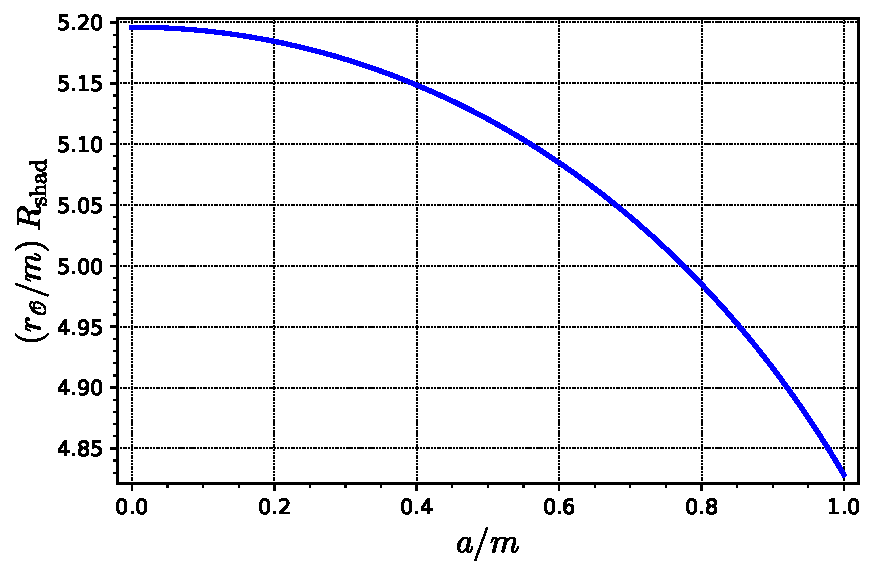
\includegraphics[height=0.28\textheight]{gik_shadow_radius_axis.pdf} }
\caption[]{\label{f:gik:shadow_radius_axis} \footnotesize
Angular radius $R_{\rm shad}$ of the (circular) critical curve of a Kerr black
hole as seen by an asymptotic inertial observer located at $r=r_{\Obs}$ on the
black hole's rotation axis, as a function of the Kerr spin parameter $a$
[Eq.~(\ref{e:gik:R_shadow_axis})]. $R_{\rm shad}$ is given in units
of $m/r_{\Obs}$ (cf. Table~\ref{t:gik:scale_factor}).
\textsl{[Figure generated by the notebook \ref{s:sam:Kerr_shadow}]}
}
\end{figure}


\subsection{Shadow for an observer on the rotation axis} \label{s:gik:shadow_rot_axis}

As stressed in Sec.~\ref{s:gik:remote_screen}, if $\th_{\Obs}\in\{0,\pi\}$,
the screen angular coordinates $(\alpha,\beta)$ can no longer be defined from the
orthonormal frame
$(\w{e}_{(\th)}, \w{e}_{(\ph)})$ associated with the Boyer-Lindquist coordinates $(\th,\ph)$.
In this case, we pick an arbitrary orthonormal
frame $(\w{e}_{(\alpha)}, \w{e}_{(\beta)})$ in the screen plane to define
$(\alpha,\beta)$.
Due to the axisymmetry of spacetime, when $\Obs$ lies on the rotation axis, the black hole
shadow is symmetric by any rotation around the screen's center. It
is therefore necessarily a disk. Its boundary, the critical curve $\mathscr{C}$,
is then a circle.
A critical null geodesic impacting the screen on $\mathscr{C}$
has necessarily $\ell=0$ [Eq.~(\ref{e:gik:obs_axis_ell_zero})]. It follows
that the parameter $r_0$ can take only a single value:
$r_0 = r_{\rm ph}^{\rm pol}$, which is
given by Eq.~(\ref{e:gik:rph_pol}). The radius of $\mathscr{C}$ is
then given by Eq.~(\ref{e:gik:alpha2_beta2_axis}), with $q=q_{\rm c}(r_{\rm ph}^{\rm pol})$:
\[
    \alpha^2 + \beta^2 = \frac{1}{r_{\Obs}^2} \left( q_{\rm c}(r_{\rm ph}^{\rm pol}) + a^2\right) .
\]
Given expression (\ref{e:gik:spher_q_r0}) of the function $q_{\rm c}$
and the fact that $r_{\rm ph}^{\rm pol}$ obeys
$(r_{\rm ph}^{\rm pol})^4 (r_{\rm ph}^{\rm pol} - 3m)^2 = a^4 (r_{\rm ph}^{\rm pol} + m)^2$,
as a solution of $\ell_{\rm c}(r_0) = 0$, we get
\be \label{e:gik:R_shadow_axis}
   \encadre{ R_{\rm shad} := \sqrt{\alpha^2 + \beta^2} = 2 \frac{m}{r_{\Obs}}
   \sqrt{\frac{r_{\rm ph}^{\rm pol}}{m}}
    \frac{\sqrt{(r_{\rm ph}^{\rm pol})^2 - a^2}}{r_{\rm ph}^{\rm pol} -  m} }
    \qquad (\th_{\Obs} = 0\ \mbox{or}\  \th_{\Obs} = \pi)
\ee
where $r_{\rm ph}^{\rm pol}$ is the function (\ref{e:gik:rph_pol}) of $(m, a)$
and the scale factor $m/r_{\Obs}$ is given for some astrophysical black holes
in Table~\ref{t:gik:scale_factor}.

\begin{example}
An example of shadow seen from the rotation axis is shown in the lower right panel of
Fig.~\ref{f:gik:shadow_a95}. The Kerr spin parameter is $a=0.95\, m$, for which
formula~(\ref{e:gik:rph_pol})
yields $r_{\rm ph}^{\rm pol} \simeq 2.493\, m$,
so that Eq.~(\ref{e:gik:R_shadow_axis}) results in
$R_{\rm shad} \simeq 4.875\, m / r_{\Obs}$.
We note that the critical curve $\mathscr{C}$ is depicted in the same color (green)
as the part of the critical curve in the other panels that crosses the $\beta$-axis,
which is expected since the critical null geodesics that reach the screen along
that axis have $\ell=0$ and thus the same parameter $r_0 = r_{\rm ph}^{\rm pol}$
as all the critical null geodesics forming $\mathscr{C}$ for $\th_{\Obs} = 0$
or $\pi$.
\end{example}

The shadow radius
$R_{\rm shad}$ is a decreasing function of $a$, which is depicted in Fig.~\ref{f:gik:shadow_radius_axis}.
Note that its variation range is pretty limited, since the limits
$\lim_{a\to 0} r_{\rm ph}^{\rm pol} = 3 m$ and $\lim_{a\to m} r_{\rm ph}^{\rm pol} = (\sqrt{2} + 1) m$
(cf. Sec.~\ref{s:gik:spher_latitudinal})
yield respectively
\be \label{e:gik:R_shad_limits}
    \lim_{a\to 0} R_{\rm shad} = 3\sqrt{3} \frac{m}{r_{\Obs}} \simeq 5.196 \, \frac{m}{r_{\Obs}}
    \quad\mbox{and}\quad
    \lim_{a\to m} R_{\rm shad} =  2(\sqrt{2} + 1) \frac{m}{r_{\Obs}}
    \simeq 4.828 \, \frac{m}{r_{\Obs}}  .
\ee
The value for $a= m$ is thus only $7\%$ lower than the value for $a= 0$.

\begin{remark}
The limit $a\to 0$ is in agreement with the result for the shadow of a
Schwarzschild black hole obtained in Sec.~\ref{s:gis:shadow}.
\end{remark}


\subsection{Shadow of an extremal Kerr black hole} \label{s:gik:shadow_extremal}

The case $a=m$ corresponds to the extremal Kerr black hole, which will be
studied in Chap.~\ref{s:exk}. However, we shall discuss its
shadow and critical curve here, by taking some appropriate limits.
For $a=m$, formulas (\ref{e:gik:spher_ell_r0})-(\ref{e:gik:spher_q_r0})
for $\ell_{\rm c}(r_0)$ and $q_{\rm c}(r_0)$ simplify significantly:
\be
    \ell_{\rm c}(r_0) = - \frac{r_0^2}{m} + 2 r_0 + m \qquad (a=m)
\ee
\be \label{e:gik:q_c_extremal}
    q_{\rm c}(r_0) = \frac{r_0^3}{m^2} ( 4 m - r_0) \qquad (a=m) .
\ee
Substituting these values into the system (\ref{e:gik:shadow_param_eq}) leads to
the screen angular coordinates determining the critical curve $\mathscr{C}$
of an extremal Kerr black hole:
\begin{subequations}
\label{e:gik:shadow_param_extremal}
\begin{align}
& \alpha =  \frac{(r_0 - m)^2 - 2 m^2}{m r_{\Obs}\sin\th_{\Obs}}  \label{e:gik:shadow_alpha_extremal} \\
& \beta = \frac{\eps_\th}{m r_{\Obs} \sin\th_{\Obs}}
        \sqrt{ r_0^3 (4 m - r_0) - m^2 \cos^2\th_{\Obs} \left[ 2 r_0(r_0 + 2 m)
                + m^2\cos^2\th_{\Obs}\right] } . \label{e:gik:shadow_beta_extremal}
\end{align}
\end{subequations}
Besides, Eq.~(\ref{e:gik:rph_pm}) yields
\be
    r_{\rm ph}^+ = m \qand r_{\rm ph}^- = 4 m \qquad (a=m) .
\ee
The range of $r_0$ is determined by $r_{\rm ph}^+ \leq r_0 \leq r_{\rm ph}^-$ and
$\tilde{\Theta}(\th_{\Obs}) \geq 0$. The last condition is equivalent to demanding that
the quantity under the square root in expression (\ref{e:gik:shadow_beta_extremal}) for $\beta$
is non-negative. This leads\footnote{The values of $r_{\rm min}$ and $r_{\rm max}$
can be computed exactly as $r_{\rm min} = \max(r_1, m)$ and $r_{\rm max} = r_2$,
where $r_1$ and $r_2$ are two roots of the quartic polynomial in $r_0$ that appears
under the square root in Eq.~(\ref{e:gik:shadow_beta_extremal}). However, doing so would
lead to complicated expressions, while a computation by numerical root finding, as in
the notebook \ref{s:sam:Kerr_shadow}, is sufficient in practice.} to some interval $[r_{\rm min}, r_{\rm max}] \subset [r_{\rm ph}^+, r_{\rm ph}^-]$.
As in the case $a<m$ treated above, we have $r_{\rm max} \leq r_{\rm ph}^-$
with $r_{\rm max} = r_{\rm ph}^- \iff \th_{\Obs} = \pi/2$.
However, $r_{\rm min}$ behaves differently. As we going to see,
$r_{\rm min} = r_{\rm ph}^+ (= m)$ for a finite-width interval of values of $\th_{\Obs}$ around $\pi/2$
and not only for $\pi/2$. To see this, let us start by noticing that expression~(\ref{e:gik:q_c_extremal})
results in $q_{\rm c}(r_{\rm ph}^-) = 0$, while $q_{\rm c}(r_{\rm ph}^+) = 3 m^2 \neq 0$.
This last result seems to contradict the fact that
$r_{\rm ph}^+$ has been
obtained in Sec.~\ref{s:gik:spher_existence} by searching for the zeros of $q_{\rm c}$.
However, the generic expression (\ref{e:gik:spher_q_r0}) for $q_{\rm c}$ has a factor $(r_0 - m)^2$
in its denominator, so that taking the limits $a\to m$ and $r_0\to r_{\rm ph}^+\ =  m$
yields the undeterminate form ``0/0''. As a consequence of $q_{\rm c}(r_{\rm ph}^+) \neq 0$,
one has $\beta\neq 0$ for $r_0 = r_{\rm ph}^+ = m$ and $|\th_{\Obs} - \pi/2|$ sufficiently small.
This implies that $r_{\rm min} = m$ for a finite range of values of $\th_{\Obs}$ around
$\pi/2$.
More precisely,
according to (\ref{e:gik:shadow_param_extremal}), the screen coordinates for $r_0 = r_{\rm ph}^+ = m$ are
\begin{subequations}
\label{e:gik:shadow_extremal_term}
\begin{align}
& \left. \alpha \right| _{r_0=m} =  - 2 \frac{m}{r_{\Obs}\sin\th_{\Obs}}  \\[1ex]
& \left. \beta \right| _{r_0=m} = \frac{\eps_\th m}{r_{\Obs} \sin\th_{\Obs}}
        \sqrt{ 3 - 6 \cos^2\th_{\Obs} - \cos^4\th_{\Obs}} .  \label{e:gik:beta_a_m_r0_m}
\end{align}
\end{subequations}
In particular, for $\th_{\Obs}=\pi/2$ (observer $\Obs$ in the equatorial plane), we get
\be \label{e:gik:shadow_extremal_term_equat}
    \left. \alpha \right| _{r_0=m}  = - 2 \, \frac{m}{r_{\Obs}}
    \qand
    \left. \beta \right| _{r_0=m} = \eps_\th \sqrt{3} \, \frac{m}{r_{\Obs}} \qquad
    \left(\th_{\Obs} = \frac{\pi}{2} \right) .
\ee
Equation~(\ref{e:gik:beta_a_m_r0_m}) shows that, for $\eps_\th = +1$,
$\left. \beta \right| _{r_0=m} > 0 \iff \th_{\rm crit} < \th_{\Obs} < \pi - \th_{\rm crit}$,
where $\th_{\rm crit}$ is such that $\cos^2\th_{\rm crit}$ is
the positive root of the quadratic polynomial $-x^2 - 6 x + 3 = 0$. We get
$\cos^2\th_{\rm crit} = 2\sqrt{3} - 3$, from which $\sin^2\th_{\rm crit} = 4 - 2\sqrt{3} = (\sqrt{3} - 1)^2$, hence
\be \label{e:gik:shadow_a1_th_crit}
    \th_{\rm crit} = \arcsin(\sqrt{3} - 1) \simeq 0.8213\, {\rm rad} \simeq 47.06^\circ .
\ee
For $\th_{\Obs} = \th_{\rm crit}$ or $\pi - \th_{\rm crit}$, we have exactly $\left. \beta \right| _{r_0=m} = 0$,
while for $\th_{\Obs} < \th_{\rm crit}$ or $\th_{\Obs} > \pi -  \th_{\rm crit}$,
$\left. \beta \right| _{r_0=m}$ is imaginary. This means that
for $\th_{\rm crit} \leq \th_{\Obs} \leq \pi - \th_{\rm crit}$, the range of the parameter $r_0$ is
$[m, r_{\rm max}]$, while for
for $\th_{\Obs} < \th_{\rm crit}$ or $\th_{\Obs} > \pi -  \th_{\rm crit}$,
the range is $[r_{\rm min}, r_{\rm max}]$ with $r_{\rm min} > m$, as for the case $\th_{\Obs} \neq \pi/2$ of the shadows with $a < m$ discussed in Sec.~\ref{s:gik:shadow_generic}. In this last case,
the critical curve is a smooth curve with $\left. \beta \right| _{r_0=r_{\rm min}} = 0$ (in addition
to $\left. \beta \right| _{r_0=r_{\rm max}} = 0$, which always holds).

\begin{figure}
\centerline{
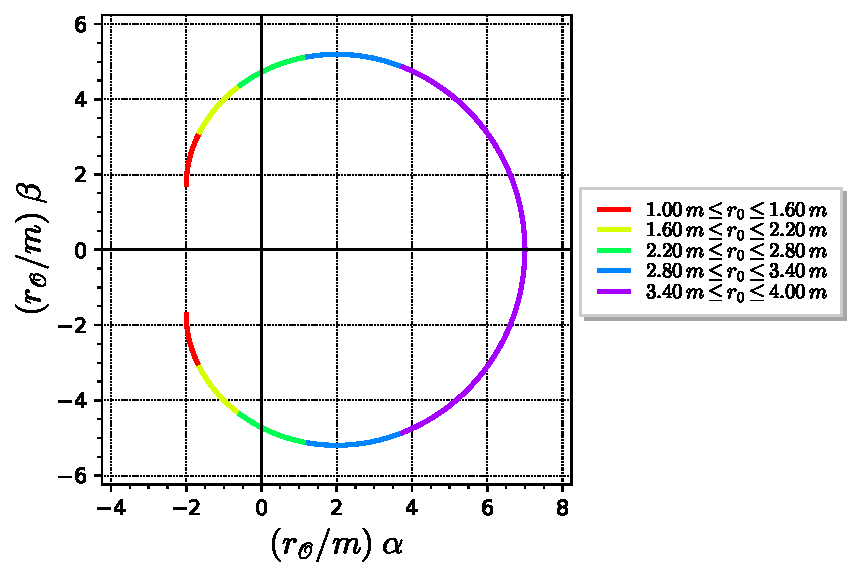
\includegraphics[height=0.28\textheight]{gik_shadow_a1_th90_part.pdf} }
\caption[]{\label{f:gik:shadow_a1_th90_part} \footnotesize
Part of the critical curve of an extremal Kerr black hole ($a=m$) in the
screen of an asymptotic inertial observer $\Obs$ in the equatorial plane
($\th_{\Obs} = \pi/2$), as defined by the
parametric equations (\ref{e:gik:shadow_param_extremal}), with $r_0\in[m, 4m]$.
The two endpoints are acheived at $r_0=m$ and are given by Eq.~(\ref{e:gik:shadow_extremal_term_equat}):
$(\bar{\alpha},\bar{\beta}) = (-2, \pm \sqrt{3}) \simeq (-2, \pm 1.732)$, where
$\bar{\alpha}:= \alpha r_{\Obs}/m$ and $\bar{\beta}:= \beta r_{\Obs}/m$.
\textsl{[Figure generated by the notebook \ref{s:sam:Kerr_shadow}]}
}
\end{figure}

Let us focus on the first case, i.e. $\th_{\rm crit} \leq \th_{\Obs} \leq \pi - \th_{\rm crit}$.
The parametric curve defined by
the system (\ref{e:gik:shadow_param_extremal}) terminates at $r_0 = m$ on the two points
given by Eq.~(\ref{e:gik:shadow_extremal_term}), or Eq.~(\ref{e:gik:shadow_extremal_term_equat})
in the particular case $\th_{\Obs} = \pi/2$ (one point for $\eps_\th=+1$, and the other one
for $\eps_\th=-1$). For $\th_{\rm crit} < \th_{\Obs} < \pi - \th_{\rm crit}$, one has
$\beta \neq 0$ at these two points, so that the curve is not closed, as one can see
on Fig.~\ref{f:gik:shadow_a1_th90_part} (drawn for $\th_{\Obs} = \pi/2$).
One may be puzzled by this feature: the shadow boundary has to be closed!
We are thus missing some critical null geodesics to complete the boundary.
It is easy to find the missing ones as soon as we remember that in the
special case $a=m$, we had found an extra family of spherical photon orbits
in Sec.~\ref{s:gik:spher_existence}: those given by Eq.~(\ref{e:gik:spher_orb_r0_eq_m}),
namely the spherical photon orbits at $r_0 = m$ that have
$\ell = 2m$. Obviously, this family cannot be parametrized by $r_0$; on the other hand,
the reduced Carter constant $q$ is a valid parameter. Since $q$ is
not constrained by Eq.~(\ref{e:gik:spher_orb_r0_eq_m}), it can take all
values in the range $[0, +\infty)$. Note that $q<0$ is not permitted here
since $\ell = 2 m > a$ [cf. property (\ref{e:gik:q_nonnegative})].
However, not any value of $q$ corresponds to a spherical photon orbit associated
with a critical null geodesic that reaches the asymptotic inertial observer $\Obs$.
Indeed, $q$ must give birth to a radial polynomial
$\mathcal{R}(r)$ positive for all $r > m$, so that the radial
motion is possible between the spherical orbit at $r_0=m$
 and the observer [condition (\ref{e:mcR_non_neg})].
Specializing expression (\ref{e:gik:mcR}) for $\mathcal{R}(r)$ to $a=m$ and $\ell=2m$,
we get
\be
    \mathcal{R}(r) = (r - m)^2 (r^2 + 2 m r - q) .
\ee
$r = m$ appears as a double root of $\mathcal{R}$, which confirms that we are dealing
with spherical photon orbits at $r_0 = m$. There are two other roots, which depend
on $q$:
\be \label{e:gik:root_rq}
    r_q^\pm = \pm \sqrt{m^2 + q} - m .
\ee
Since $q\geq 0$, we have $r_q^+ \geq 0$ and $r_q^- \leq - 2m$.
It is then clear (cf. Fig.~\ref{f:gik:R_a_1_l_2m}) that
\be
     \left( \forall r \in (m, +\infty),\quad  \mathcal{R}(r) > 0 \right) \iff r_q^+ \leq m .
\ee
The critical value is $r_q^+ = m$, which correspond to $q = 3 m^2$ (red curve
in Fig.~\ref{f:gik:R_a_1_l_2m}). $r=m$ is then a triple root of $\mathcal{R}$:
$q = 3 m^2 \implies \mathcal{R}(r) = ( r - m)^3 (r + 3m)$. Since $r_q^+$
is an increasing function of $q$, we conclude that
\begin{greybox}
For $a=m$, a critical null geodesic
of constants of motion $(\ell, q)$ can reach the asymptotic region $r\gg m$
from the vicinity of a spherical photon orbit at $r_0 = m$ iff
\be \label{e:gik:critical_from_NHEK}
    \ell = 2 m \qand 0 \leq q \leq 3 m^2 .
\ee
\end{greybox}

\begin{figure}
\centerline{
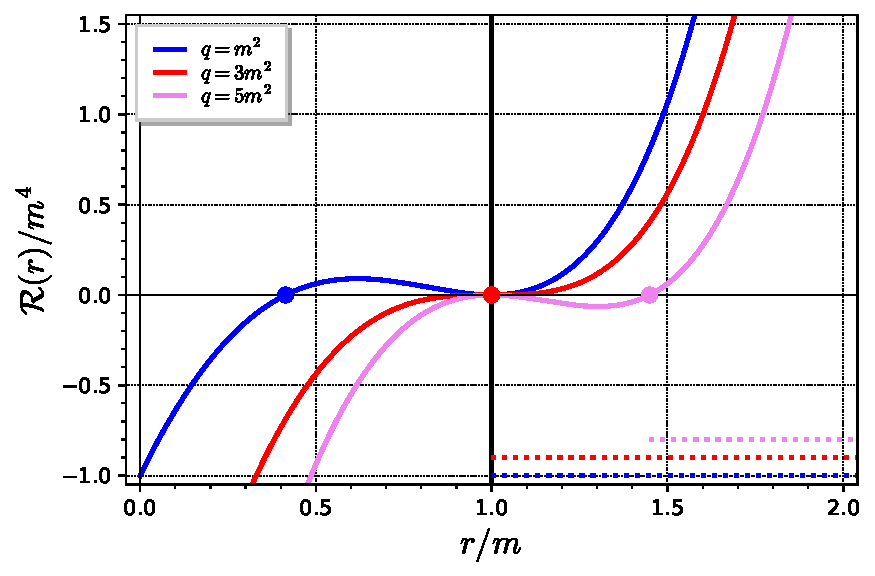
\includegraphics[height=0.28\textheight]{gik_R_a_1_l_2m.pdf} }
\caption[]{\label{f:gik:R_a_1_l_2m} \footnotesize
Radial polynomial $\mathcal{R}(r)$ for $a=m$, $\ell=2m$ and three values of $q$.
All the polynomials have a double root at $r=m$ and
the dots mark the root $r_q^+$ [Eq.~(\ref{e:gik:root_rq})], the fourth root $r_q^- \leq - 2m$ being out of the
figure's scope. The dotted horizontal lines indicate the range of $r$
where a null geodesic motion to the asymptotic inertial observer is possible.
\textsl{[Figure generated by the notebook \ref{s:sam:Kerr_shadow}]}
}
\end{figure}

Furthermore, such a critical null geodesic can reach the asymptotic inertial
observer $\Obs$, who is located at $\th = \th_{\Obs}$, only if the
$\tilde{\Theta}$ function associated with $(\ell,q)$ obeys $\tilde{\Theta}(\th_{\Obs}) \geq 0$.
Setting $a=m$ and $\ell=2m$ into expression (\ref{e:gik:tTheta}) for $\tilde{\Theta}$,
we get the criterion
\be \label{e:gik:critical_NHEK_to_Obs}
    q \geq \frac{3 + \cos^2\th_{\Obs}}{\tan^2\th_{\Obs}} \, m^2 .
\ee
The screen angular coordinates corresponding to the critical null geodesic
are obtained by plugging the
above values of $\ell$ and $q$, as well as $a=m$, into formulas (\ref{e:gik:screen_alpha_beta}):
\begin{subequations}
\label{e:gik:alpha_beta_NHEK_line}
\begin{align}
& \alpha = - \frac{2 m}{r_{\Obs}\sin\th_{\Obs}}  \\
&  \beta = \frac{\eps_\th m}{r_{\Obs}\sin\th_{\Obs}} \sqrt{ \frac{q}{m^2}\sin^2\th_{\Obs}
 - \cos^2\th_{\Obs} \left( 3 + \cos^2\th_{\Obs} \right)  },
 \quad \frac{3 + \cos^2\th_{\Obs}}{\tan^2\th_{\Obs}}  \leq \frac{q}{m^2} \leq 3 .
\end{align}
\end{subequations}
The system (\ref{e:gik:alpha_beta_NHEK_line}) defines a curve parametrized by $q$,
with the range of $q$ obtained by combining (\ref{e:gik:critical_from_NHEK}) and (\ref{e:gik:critical_NHEK_to_Obs}).
For $\Obs$ in the equatorial plane $(\th_{\Obs} = \pi/2)$, this parametric equation
simplifies to
\be
    \alpha = - 2 \frac{m}{r_{\Obs}}
    \qand
    \beta = \eps_\th \frac{m}{r_{\Obs}} \sqrt{ \frac{q}{m^2} },
    \quad 0 \leq \frac{q}{m^2} \leq 3  \qquad\left( \th_{\Obs} = \frac{\pi}{2} \right) .
\ee
In all cases, the curve (\ref{e:gik:alpha_beta_NHEK_line})
is actually a segment of a vertical straight line on $\Obs$'s screen, since it
has $\alpha=\mathrm{const}$. Following Ref.~\cite{GrallLS18},
we shall call this segment the \defin{NHEK line}\index{NHEK!line}, \emph{NHEK} standing
for \emph{Near Horizon Extremal Kerr}, given that spherical photon orbits
at $r_0=m$ are close\footnote{Despite they have the same radial coordinate as the horizon ($r_+=m$ for $a=m$),
the spherical photon orbits at $r_0=m$ are not located
on the horizon, for $r$ fails to be a well-behaved coordinate at $r=m$ in
the extremal Kerr geometry, as we shall discuss in Chap.~\ref{s:exk}.}
to the event horizon of the extremal Kerr black hole.
The key feature is that the end points
of the NHEK line, which are obtained for $q/m^2 = 3$,
are exactly the two points defined by Eq.~(\ref{e:gik:shadow_extremal_term}),
i.e. the end points of the curve parametrized by $r_0$ (cf. Fig.~\ref{f:gik:shadow_a1_th90_part}).
By adding the NHEK line, we are thus
closing the boundary of the black hole shadow! The result is shown in Fig.~\ref{f:gik:shadow_a1},
where the NHEK line is drawn in maroon on the left edge of the plots
for $\th_{\Obs} = \pi/2$ and $\th_{\Obs} = \pi/3 > \th_{\rm crit}$.

\begin{figure}
\begin{center}
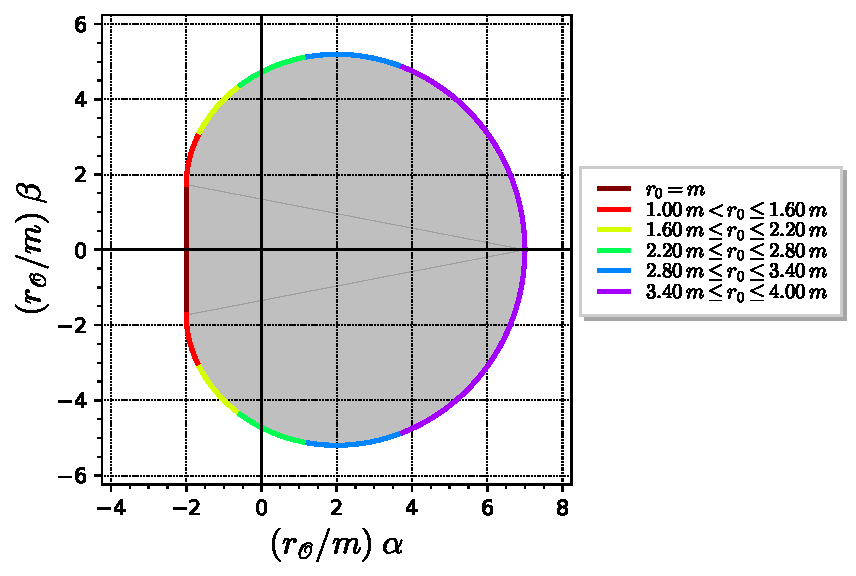
\includegraphics[height=0.28\textheight]{gik_shadow_a1_th90.pdf} \\[1ex]
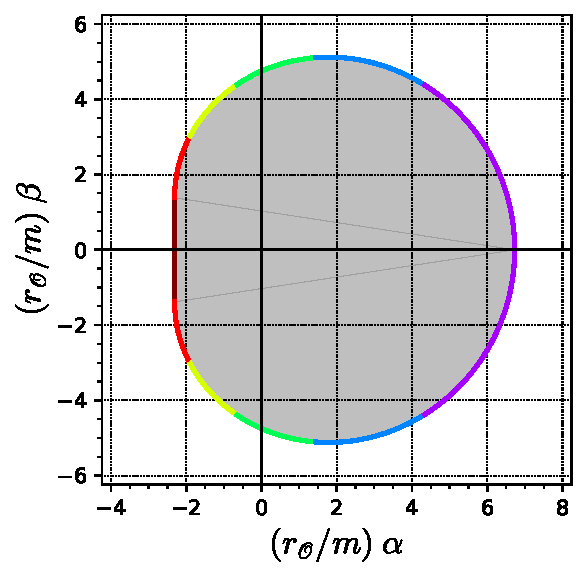
\includegraphics[height=0.28\textheight]{gik_shadow_a1_th60.pdf}\qquad
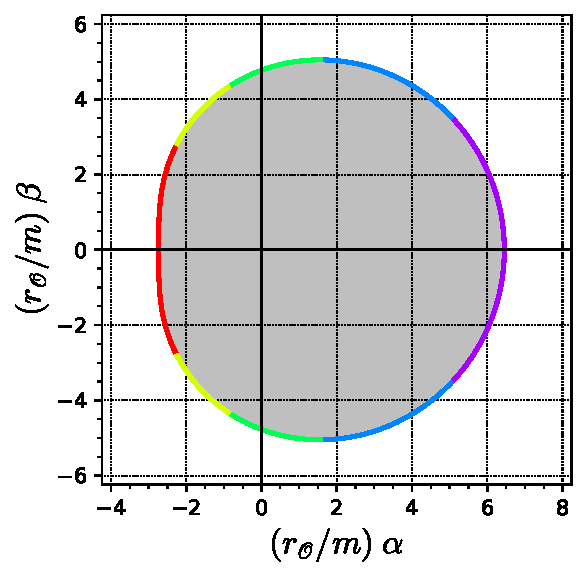
\includegraphics[height=0.28\textheight]{gik_shadow_a1_th_crit.pdf}
\end{center}
\caption[]{\label{f:gik:shadow_a1} \footnotesize
Critical curve $\mathscr{C}$ (colored curve) and shadow (grey area)
of an extremal Kerr black hole on the screen of an asymptotic
inertial observer $\Obs$ located at $r=r_{\Obs}$ and $\th=\th_{\Obs}$, for three
values of $\th_{\Obs}$: $\th_{\Obs} = \pi/2$ ($\Obs$ in the equatorial plane; upper panel),
$\th_{\Obs} = \pi/3$ (lower left) and $\th_{\Obs} = \th_{\rm crit} = \arcsin(\sqrt{3} - 1) \simeq 0.821$
[Eq.~(\ref{e:gik:shadow_a1_th_crit})]. The NHEK line (plotted in maroon) is present in
the first two images, while
it is vanishing in the third one (marginal case), since there is no NHEK line in $\mathscr{C}$ for $\th < \th_{\rm crit}$ or $\th > \pi -  \th_{\rm crit}$.
As in Fig.~\ref{f:gik:shadow_a95},
the color code corresponds to some selected ranges for the parameter $r_0$
of the critical null geodesics forming $\mathscr{C}$.
\textsl{[Figure generated by the notebook \ref{s:sam:Kerr_shadow}]}
}
\end{figure}

\subsubsection{Cardioid shape}

As seen from Fig.~\ref{f:gik:shadow_a1}, the departure of the critical curve
$\mathscr{C}$ from a perfect circle is maximal when the observer lies in the equatorial
plane, i.e. when $\th_{\Obs} = \pi/2$. The critical curve is often said to have
a \emph{D-shape} (from the letter D). It is interesting that this shape
corresponds actually to a simple mathematical curve: the convex hull of a
cardioid \cite{FarahPJB20}.
Indeed, for $\th_{\Obs} = \pi/2$, equations (\ref{e:gik:shadow_param_extremal}),
which govern the part of $\mathscr{C}$ parametrized by $r_0$,
simplify to
\begin{subequations}
\label{e:gik:shadow_a1_equat}
\begin{align}
    & \alpha = \frac{(r_0 - m)^2 - 2 m^2}{m r_{\Obs}} \label{e:gik:shadow_alpha_a1_equat} \\
    & \beta = \frac{\eps_\th}{m r_{\Obs}} r_0 \sqrt{r_0(4 m - r_0)} . \label{e:gik:shadow_beta_a1_equat}
\end{align}
\end{subequations}
Let us then extract $r_0$ from Eq.~(\ref{e:gik:shadow_alpha_a1_equat}):
\[
    r_0 = m \left( 1 + \sqrt{2 + \frac{r_{\Obs}}{m}\alpha} \right)
\]
and substitute it into the square of Eq.~(\ref{e:gik:shadow_beta_a1_equat}); we get (using $\eps_\th^2 = 1$)
\be \label{e:gik:beta2_alpha}
    \beta^2 = \frac{m^2}{r_{\Obs}^2} \left( 1 + \sqrt{2 + \frac{r_{\Obs}}{m}\alpha}\,  \right) ^3
    \left( 3 -  \sqrt{2 + \frac{r_{\Obs}}{m}\alpha} \, \right) .
\ee
At this stage, it is worth to introduce explicitely the rescaled angular coordinates used
in Figs.~\ref{f:gik:shadow_a1_th90_part} and \ref{f:gik:shadow_a1}:
\be \label{e:gik:def_bar_alp_bet}
    \bar{\alpha} := \frac{r_{\Obs}}{m} \alpha \qand
    \bar{\beta} := \frac{r_{\Obs}}{m} \beta .
\ee
Then, by expanding its right-hand side, we can rewrite Eq.~(\ref{e:gik:beta2_alpha}) as
\be \label{e:gik:beta2_alpha_expanded}
    \bar{\beta}^2 = - \bar{\alpha}^2 + 2 \bar{\alpha} + 8 \sqrt{\bar{\alpha} + 2} + 11 .
\ee
Let us introduce new screen coordinates $(\hat{\alpha}, \hat{\beta})$ by
shifting the origin to $(\bar{\alpha},\bar{\beta}) = (-1, 0)$:
\be
    \hat{\alpha} := \bar{\alpha} + 1  \qand
    \hat{\beta} := \bar{\beta} .
\ee
We can then recast Eq.~(\ref{e:gik:beta2_alpha_expanded}) as
\be \label{e:gik:al2be2_prov}
    \hat{\alpha}^2 + \hat{\beta}^2 - 4 \hat{\alpha} = 8 \left( \sqrt{\hat{\alpha} + 1} + 1 \right).
\ee
The square of this expression is
$(\hat{\alpha}^2 + \hat{\beta}^2  - 4 \hat{\alpha})^2 =
    64 ( \hat{\alpha} + 2 \sqrt{\hat{\alpha} + 1} + 2 )$.
Using Eq.~(\ref{e:gik:al2be2_prov}) to get rid of the square root, we obtain
\be \label{e:gik:cardioid_Cartesian}
   \left( \hat{\alpha}^2 + \hat{\beta}^2  - 4 \hat{\alpha} \right)^2 =
    16 \left(  \hat{\alpha}^2 + \hat{\beta}^2 \right) .
\ee
The reader may have recognized the Cartesian equation of a cardioid\index{cardioid}. To put it
in a more familiar form, let us introduce the polar coordinates $(\rho,\phi)$
defined by $\rho^2 := \hat{\alpha}^2 + \hat{\beta}^2$, $\cos\phi := \hat{\alpha}/\rho$
and $\sin\phi := \hat{\beta}/\rho$.
Then Eq.~(\ref{e:gik:cardioid_Cartesian}) becomes
$(\rho^2 - 4 \rho\cos\phi )^2 = 16 \rho^2$,
which is equivalent to $(\rho - 4\cos\phi)^2 = 16$, i.e.
to $\rho = \pm 4 + 4\cos\phi$.
Given that $\rho \geq 0$, the $\pm$ sign must be $+$, so that we end up with
\be
    \rho = 4 \left( 1 + \cos\phi \right) .
\ee
We recognize the polar equation of a cardioid\index{cardioid}, generated by a circle of radius 2 rolling around a
circle of the same radius and centered at $(\hat{\alpha},\hat{\beta}) = (2,0) \iff
(\bar{\alpha},\bar{\beta}) = (1, 0)$.

\begin{figure}
\centerline{
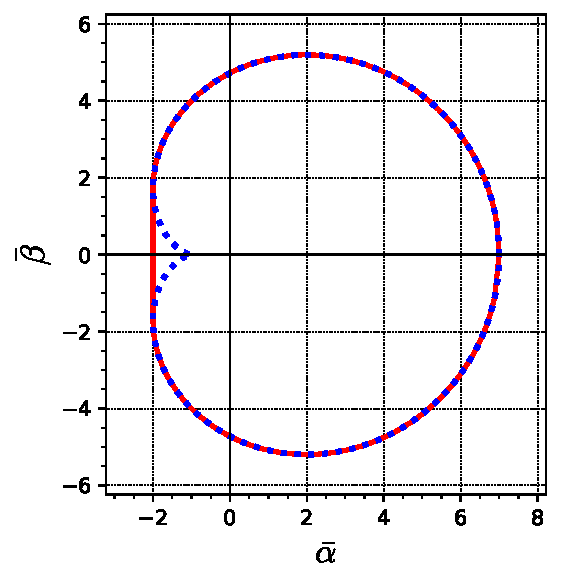
\includegraphics[height=0.28\textheight]{gik_shadow_cardioid.pdf} }
\caption[]{\label{f:gik:shadow_cardioid} \footnotesize
Cardioid defined by the polar equation $\rho = 4 \left( 1 + \cos\phi \right)$ (dotted blue curve)
and critical curve of an extremal Kerr black hole seen from the equatorial
plane (red curve). The screen coordinates $(\bar{\alpha},\bar{\beta})$ are
defined by Eq.~(\ref{e:gik:def_bar_alp_bet}), while $(\rho,\phi)$ are polar
coordinates around the point $(\bar{\alpha},\bar{\beta})=(-1,0)$, i.e.
$\rho := \sqrt{(\bar{\alpha}+1)^2 + \bar{\beta}^2}$ and $\sin\phi := \bar{\beta}/\rho$.
\textsl{[Figure generated by the notebook \ref{s:sam:Kerr_shadow}]}
}
\end{figure}

As it is clear from the starting point of the above calculation, the cardioid corresponds only to the part of the critical curve parametrized by $r_0$, i.e. the part depicted in
Fig.~\ref{f:gik:shadow_a1_th90_part}. It does not reproduce the NHEK line. Actually, adding
the NHEK line results in the convex hull of the cardioid, as shown in Fig.~\ref{f:gik:shadow_cardioid}.

\begin{remark}
It is amusing to note that the cardioid is involved in two optical phenomena of
very distinct origin: in classical optics, it appears as
the caustic generated by reflection of light on a circular material, such as a bowl or
a coffee cup, and at the same time, it delineates the shadow of
some black holes of general relativity.
\end{remark}

\begin{remark}
For $\th_{\Obs}\neq \pi/2$, the critical curve $\mathscr{C}$ of the extremal Kerr black hole
is no longer a cardioid. It is however still a quartic algebraic curve,
i.e. $(\bar{\alpha},\bar{\beta})$ obey an algebraic equation of degree 4,
as in Eq.~(\ref{e:gik:cardioid_Cartesian}). Moreover, $\mathscr{C}$ is a classical elementary curve,
namely a \emph{Cartesian oval}\index{Cartesian!oval}, also
known as \emph{oval of Descartes}\index{oval!Cartesian --}\index{oval!of Descartes},
as shown in Ref.~\cite{GrallL20c}. More precisely, $\mathscr{C}$ is exactly such an oval
for $\th_{\Obs} \leq  \th_{\rm crit}$ or $\th_{\Obs} \geq \pi - \th_{\rm crit}$.
For $\th_{\rm crit}  < \th_{\Obs} < \pi - \th_{\rm crit}$, i.e. when the NHEK line is present,
$\mathscr{C}$ is the convex hull of a Cartesian oval.
\end{remark}

\begin{figure}
\begin{center}
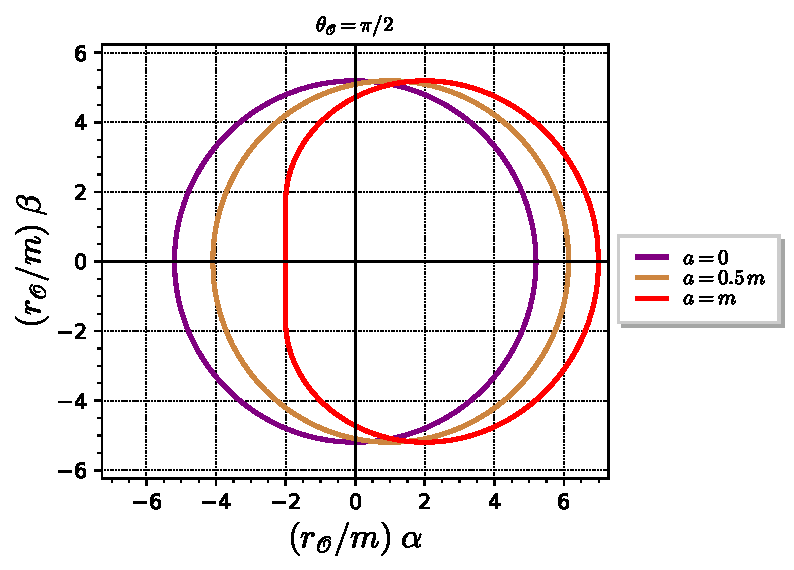
\includegraphics[height=0.28\textheight]{gik_shadow_comp_th90.pdf} \\[1ex]
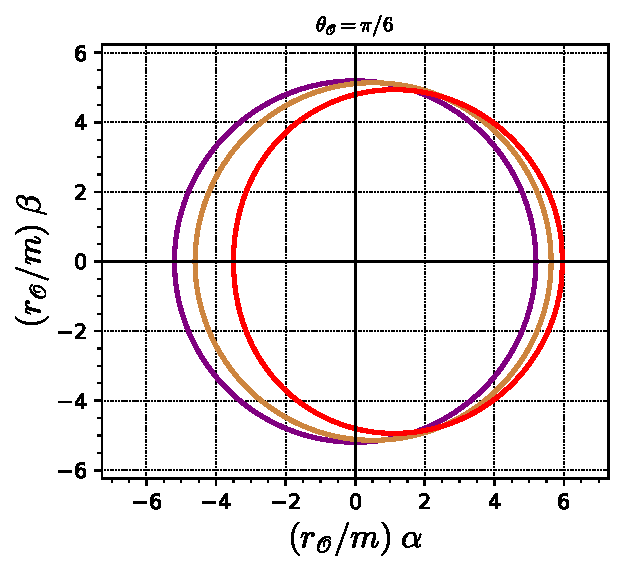
\includegraphics[height=0.28\textheight]{gik_shadow_comp_th30.pdf}\qquad
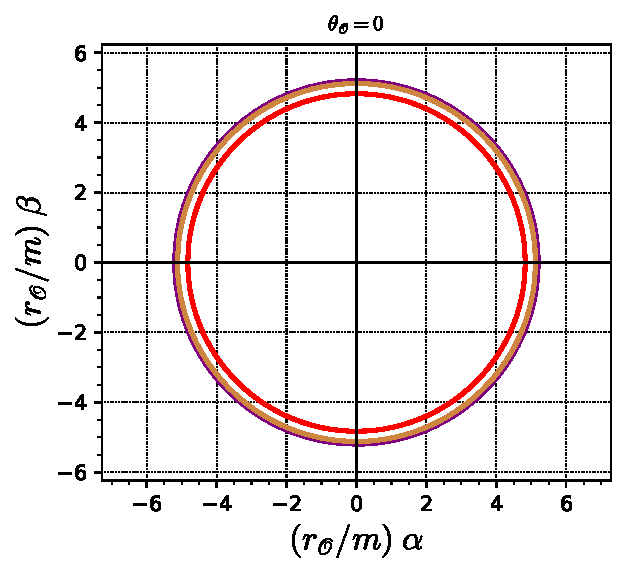
\includegraphics[height=0.28\textheight]{gik_shadow_comp_th00.pdf}
\end{center}
\caption[]{\label{f:gik:shadow_comp_th} \footnotesize
Critical curves for different values of $a$ at fixed observer's inclination
angle: $\th_{\Obs} = \pi/2$ (top panel),   $\th_{\Obs} = \pi/6$ (lower left panel)
and $\th_{\Obs} = 0$ (lower right panel).
\textsl{[Figure generated by the notebook \ref{s:sam:Kerr_shadow}]}
}
\end{figure}



\subsection{Comparing the critical curves at fixed inclination}

From an observational point of view, it may happen that the inclination angle
$\th_{\Obs}$ is known, as we shall see for M87* in Sec.~\ref{s:gik:M87_image}.
Figure~\ref{f:gik:shadow_comp_th} compares then the critical curves at a fixed
value of $\th_{\Obs}$ for various values of the black hole spin parameter $a$.
For $\th_{\Obs}=0$, we recover the feature found in Sec.~\ref{s:gik:shadow_rot_axis},
namely that the critical curve depends very weakly on the spin.

\begin{hist}
The critical curve of a Kerr black hole has been computed
first by James M.~Bardeen\index{Bardeen, J.M.} in 1972 \cite{Barde73}
(cf. the historical note on p.~\pageref{h:gis:bh_shadow}), in the form
of the parametric system (\ref{e:gik:shadow_param_eq}). He wrote:
\emph{The rim of the ``black hole''\footnote{For Bardeen, ``black hole''
(with quotes) stands for the black spot on the observer's screen.}
corresponds to photon trajectories which
are marginally trapped by the black hole; they spiral around many times before
they reach the observer. It is conceptually interesting, if not astrophysically
very important, to calculate the precise apparent shape of the black hole}.
Fifty years later, with the first image from the Event Horizon Telescope~\cite{EHT19a,Wielg_al20}, this has become astrophysically important!
For $a=m$ and $\th_{\Obs}=\pi/2$, Bardeen derived the
system (\ref{e:gik:shadow_a1_equat}) governing the part of the critical
curve parametrized by $r_0$. For the NEHK line, he simply
noted\footnote{$q$ is denoted by $\eta$ by Bardeen.}: \emph{The non-uniform
nature of the limit $a\to m$ allows $q$ to range between
$0$ and $3m^2$ at $r=m$}.
Bardeen presented then
a plot of the resulting critical curve
(Fig.~6 in Ref.~\cite{Barde73})
similar to that
shown in the top panel of Fig.~\ref{f:gik:shadow_a1}.

The term \emph{black hole shadow} for the interior of the critical curve
has been coinded by Heino Falcke\index{Falcke, H.}, Fulvio Melia\index{Melia, F.} and Eric Agol\index{Agol, E.} in 2000 \cite{FalckMA00}, cf. the historical note on p.~\pageref{h:gik:disk_images}.
\end{hist}


%%%%%%%%%%%%%%%%%%%%%%%%%%%%%%%%%%%%%%%%%%%%%%%%%%%%%%%%%%%%%%%%%%%%%%%%%%%%%%%

\section{Images} \label{s:gik:images}

\subsection{Multiples images}

The main features of images of a single luminous source on the screen of a remote observer in Kerr spacetime are similar to those obtained for Schwarzschikd spacetime in Sec.~\ref{s:gis:images}.
In particular, a single source, wherever localized in the black hole exterior (region $\M_{\rm I}$),
gives birth to two infinite sequences of images on the screen of the asymptotic inertial observer,
both of them converging to the critical curve $\mathscr{C}$. Typically, one sequence is with
$\ell>0$ and the other one with $\ell < 0$.
Each image in a given sequence can be labelled by the number $n$ of round trip around the black hole
and is dimmer and dimmer as $n$ increases.



\subsection{Image of an accretion disk}

Beside gravitational waves, the main way of observing black holes is through
the electromagnetic radiation from material orbiting around them,
either in the form of stars, as in the case of Sgr~A*, or in the
form of an accretion disk\index{accretion!disk} \cite{AbramF13}.
In the latter case, most observations are spectrum from unresolved accretion disks.
However recently, the Event Horizon Telescope team has produced the first
resolved image of an accretion disk in the close vicinity of the black hole M87*
\cite{EHT19a,Wielg_al20}.

Figures~\ref{f:gik:img_disk_a50} and \ref{f:gik:img_disk_a95}
present some computed images of an accretion disk around a Kerr black hole,
for respectively $a=0.5\, m$ and $a=0.95\, m$.
The accretion disk is a simple model developed in Ref.~\cite{VinceWAGLPG21}.
It consists in a geometrically thick and optically thin accretion disk with
an opening angle of $1.1\; {\rm rad} \simeq 63^\circ$ and an inner radius located at the prograde
ISCO (cf. Sec.~\ref{s:gek:circ_orb_stab}), which is
$r_{\rm ISCO}^+ \simeq 4.233 \, m$
for $a=0.5\, m$ (Fig.~\ref{f:gik:img_disk_a50})
and
$r_{\rm ISCO}^+ \simeq 1.937\, m$
for $a=0.95\, m$ (Fig.~\ref{f:gik:img_disk_a95}). The disc is in Keplerian rotation
and the electromagnetic emission is due to thermal synchrotron radiation
of electrons in the local magnetic field (see Ref.~\cite{VinceWAGLPG21} for details).
The images have been generated by the open-source ray-tracing code
\textsf{Gyoto}\index{Gyoto} \cite{VincePGP11} (cf. Appendix~\ref{s:gyo}).



\begin{figure}
\begin{tabular}{ccc}
\vcentertab{$\th_{\Obs} = 0$} &
\vcentertab{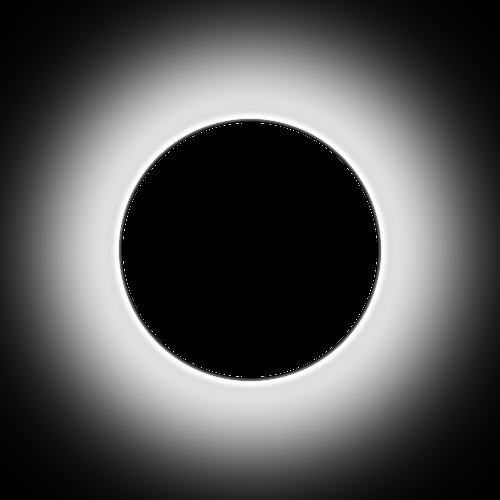
\includegraphics[width=0.35\textwidth]{gik_a50_th00.png}}&
\vcentertab{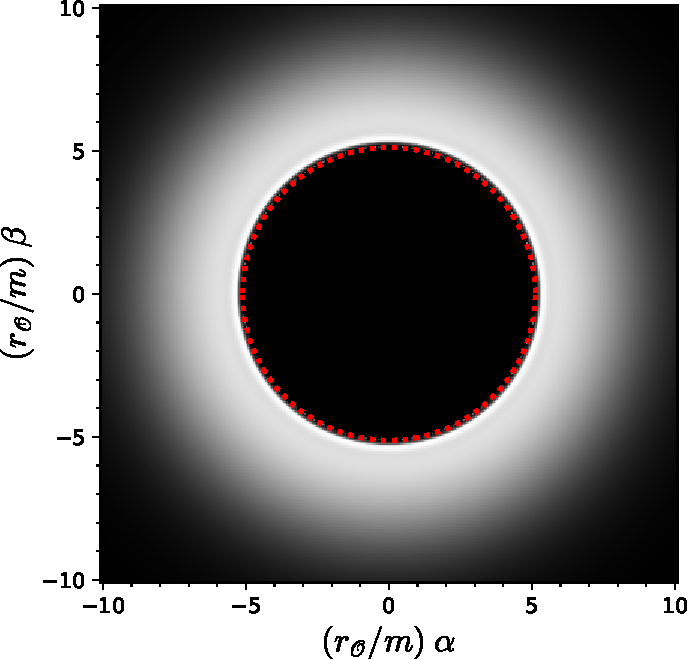
\includegraphics[width=0.37\textwidth]{gik_a50_th00_crit.pdf}}\\
\vcentertab{$\th_{\Obs} = \pi/6$} &
\vcentertab{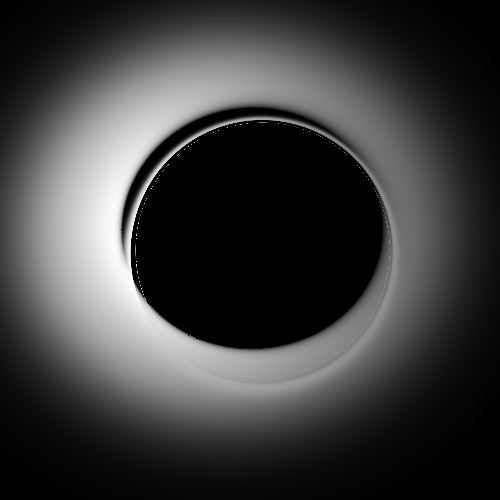
\includegraphics[width=0.35\textwidth]{gik_a50_th30.png}} &
\vcentertab{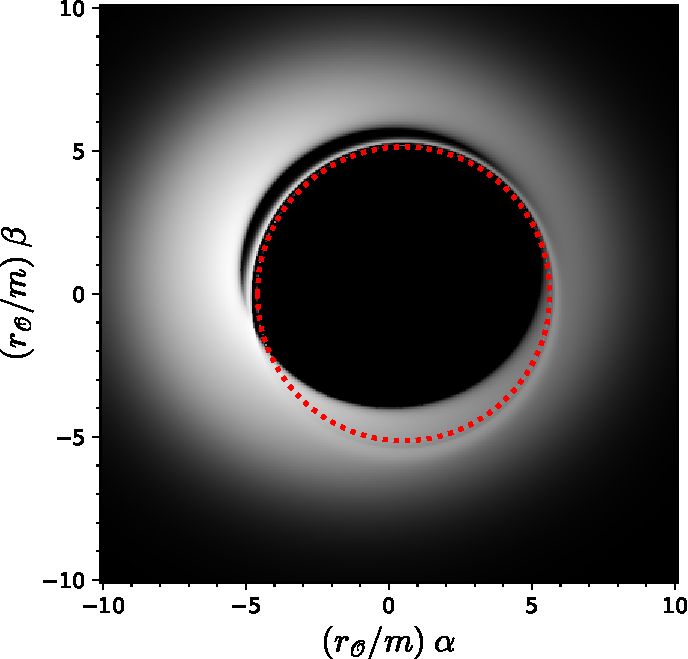
\includegraphics[width=0.37\textwidth]{gik_a50_th30_crit.pdf}}\\
\vcentertab{$\th_{\Obs} = \pi/3$} &
\vcentertab{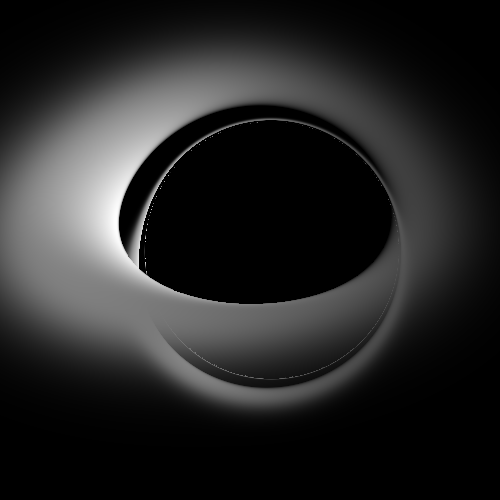
\includegraphics[width=0.35\textwidth]{gik_a50_th60.png}} &
\vcentertab{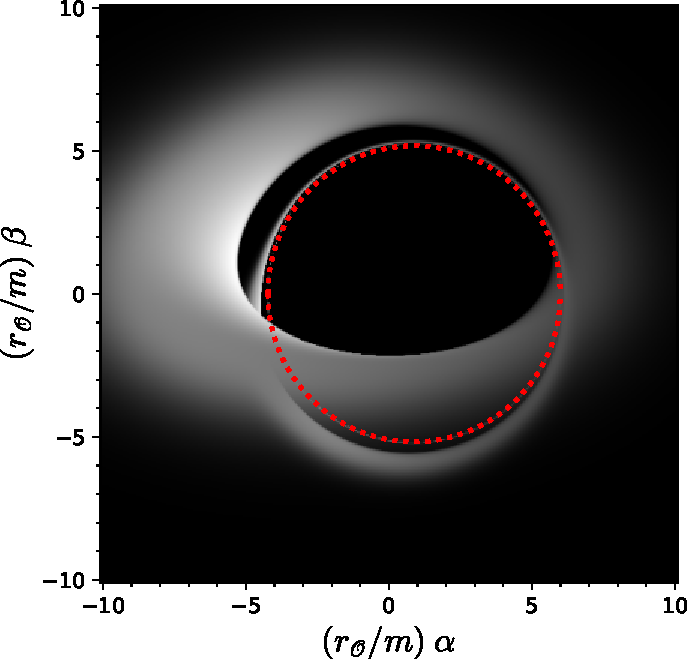
\includegraphics[width=0.37\textwidth]{gik_a50_th60_crit.pdf}}\\
\vcentertab{$\th_{\Obs} = \pi/2$} &
\vcentertab{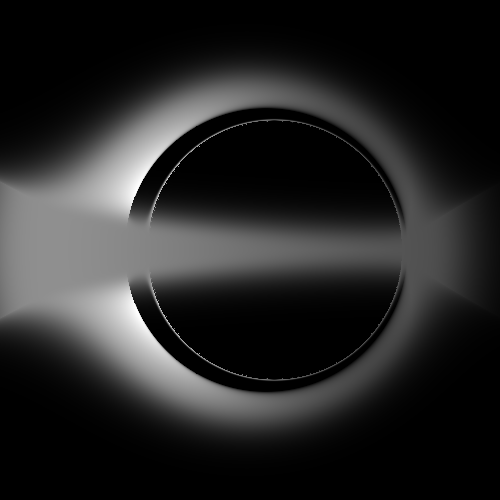
\includegraphics[width=0.35\textwidth]{gik_a50_th90.png}} &
\vcentertab{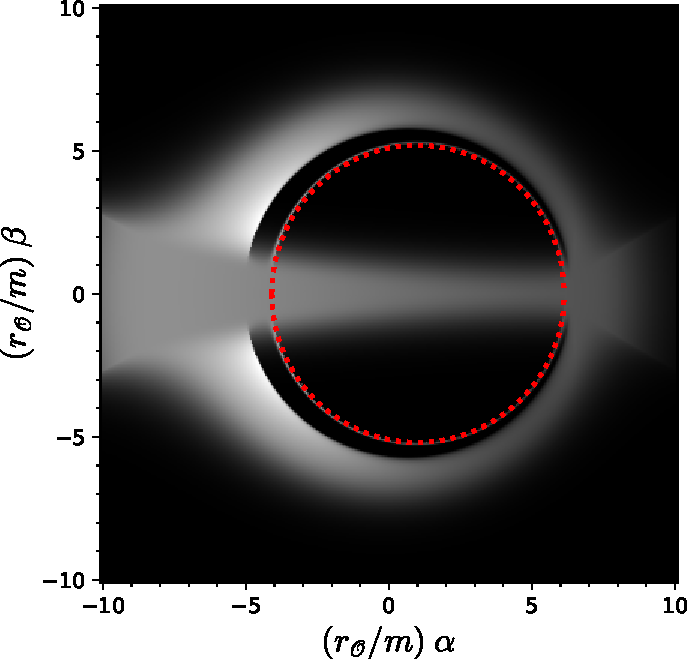
\includegraphics[width=0.37\textwidth]{gik_a50_th90_crit.pdf}}
\end{tabular}
\caption[]{\label{f:gik:img_disk_a50} \footnotesize
Images of a thick accretion disk around a Kerr black bole with $a=0.5\, m$
for three observer's inclination angles $\th_{\Obs}$. The right column shows the critical curve (red dotted line)
superposed on the image.
\textsl{[Images produced by \textsf{Gyoto} with the input
files given in Sec.~\ref{s:gyo:Kerr}; the addition of the
critical curve in the right column has been performed by means of the
\textsf{SageMath} notebook \ref{s:sam:Kerr_images}]}
}
\end{figure}

\begin{figure}
\begin{tabular}{ccc}
\vcentertab{$\th_{\Obs} = 0$} &
\vcentertab{\includegraphics[width=0.35\textwidth]{gik_a95_th00.png}}&
\vcentertab{\includegraphics[width=0.37\textwidth]{gik_a95_th00_crit.pdf}}\\
\vcentertab{$\th_{\Obs} = \pi/6$} &
\vcentertab{\includegraphics[width=0.35\textwidth]{gik_a95_th30.png}} &
\vcentertab{\includegraphics[width=0.37\textwidth]{gik_a95_th30_crit.pdf}}\\
\vcentertab{$\th_{\Obs} = \pi/3$} &
\vcentertab{\includegraphics[width=0.35\textwidth]{gik_a95_th60.png}} &
\vcentertab{\includegraphics[width=0.37\textwidth]{gik_a95_th60_crit.pdf}}\\
\vcentertab{$\th_{\Obs} = \pi/2$} &
\vcentertab{\includegraphics[width=0.35\textwidth]{gik_a95_th90.png}} &
\vcentertab{\includegraphics[width=0.37\textwidth]{gik_a95_th90_crit.pdf}}
\end{tabular}
\caption[]{\label{f:gik:img_disk_a95} \footnotesize
Same as Fig.~\ref{f:gik:img_disk_a50} but for $a = 0.95\, m$
and the images in the right column using a log scale to reveal the faint parts.
The critical curves are the same as in Fig.~\ref{f:gik:shadow_a95}.
}
\end{figure}


Figure~\ref{f:gik:img_disk_a50} provides images for moderate black hole spin: $a = 0.5\, m$.
For a given inclination $\th_{\Obs}$, the images are rather similar to those
of the accretion disk around a Schwarzschild
black hole displayed in Fig.~\ref{f:gis:disk_images}. In particular, one notices
three images of the disk, as in Fig.~\ref{f:gis:disk_images}: a broad primary image,
a secondary image with a narrow annular shape
and a thin tertiary image appearing as a very thin ring, which is dotted by lack of
resolution.
The qualitative explanation of these images is basically the same as in the Schwarzschild case.
In particular, for the disk face-on view ($\th_{\Obs} = 0$), one could
use a figure similar to Fig.~\ref{f:gis:disk_face_on}, with the
orange null geodesics generating the primary image, the brown ones
the secondary image and the red ones the tertiary image. The green circle
would then mark the location of polar spherical photon orbits,
at $r_{\rm ph}^{\rm pol} \simeq 2.883\, m$ for $a=0.5\, m$,
since only the $\ell=0$ critical null geodesics matter for $\th_{\Obs} = 0$.
There is actually an infinite sequence of images, the
image of order $n$ being generated by null geodesics that have performed
$n$ half-turns around the sphere $r=r_{\rm ph}^{\rm pol}$ before
leaving toward the observer, with $n=0$ corresponding to the primary image.
A confirmation of this interpretation is provided by the superposition
of the critical curve $\mathscr{C}$ onto the image, as the red dotted line in the
right column of Fig.~\ref{f:gik:img_disk_a50}. The tertiary image ($n=2$) is then
almost undistinguishable from $\mathscr{C}$, in agreement with the exponential
convergence of high order images to $\mathscr{C}$. This exponential convergence
has been established for $a=0$ by Eq.~(\ref{e:gis:bn_sequence}),
but it holds as well for $a \neq 0$ \cite{GrallL20a}.

Another common feature with the Schwarzschild images of Fig.~\ref{f:gis:disk_images}
is the left part of the primary image being brighter than the right part
as soon as $\th_{\Obs} \neq 0$. As discussed in Sec.~\ref{s:gis:image_disk},
this is due to the Doppler boosting resulting from the rotation of the
accretion disk, the left part moving towards the observer, while the right
part is receding.

A difference with the Schwarzschild images discussed in Sec.~\ref{s:gis:image_disk}
is that in the current case, the disk is not confined to the equatorial
plane, being geometrically thick, and moreover it is optically thin. This
means that a given null geodesic touching the screen ``carries'' not only a photon
from the disk's surface but also photons from the disk interior, actually all the photons
emitted along the path of the geodesic inside the disk. This cumulative property
results in a enhanced brightness of the secondary image and makes it appear
as a relatively bright ring, as it is clear on the $\th_{\Obs}=0$ and
$\th_{\Obs}=\pi/6$ images of Fig.~\ref{f:gik:img_disk_a50}. Another consequence
of optical thinness is that the bottom part of the secondary and tertiary
images are not blocked at high inclination by the part of the accretion
disk standing in the foreground, as they are in the images of Fig.~\ref{f:gis:disk_images},
which have been obtained for an optically thick disk model.

Another difference between the two sets of
images is that in
Fig.~\ref{f:gik:img_disk_a50} the inner boundary of the top part of the primary
image is closer to the secondary image than in Fig.~\ref{f:gis:disk_images}
(for $\th_{\Obs} = 0$, the primary and secondary images in Fig.~\ref{f:gik:img_disk_a50} seem even to touch each other). This is
a mere consequence of the inner radius of the accretion disk being closer to the
black hole in Fig.~\ref{f:gik:img_disk_a50}, since $r_{\rm ISCO}^+ \simeq 4.233 \, m$
for $a=0.5\, m$ and $r_{\rm ISCO}^+ = 6 m$
for $a=0$.

\begin{figure}
\centerline{\includegraphics[height=0.28\textheight]{gik_rISCO_rph.pdf}}
\caption[]{\label{f:gik:rISCO_rph} \footnotesize
Radius of the timelike prograde ISCO, $r_{\rm ISCO}^+$ [Eq.~(\ref{e:gek:r_ISCO})], compared
with the radii of the prograde and retrograde outer circular photon orbits, $r_{\rm ph}^+$
and $r_{\rm ph}^-$ [Eq.~(\ref{e:gik:rph_pm})] and
the radius of polar spherical photon orbits, $r_{\rm ph}^{\rm pol}$ [Eq.~(\ref{e:gik:rph_pol})].
\textsl{[Figure generated by the notebook \ref{s:sam:Kerr_images}]}
}
\end{figure}

In the images of Fig.~\ref{f:gik:img_disk_a50}, the interior of the critical
curve, i.e. the black hole shadow according to the definition given in Sec.~\ref{s:gik:shadow_generic}, appears black, except when crossed by the bottom of the primary
image, which arises from the foreground part of the disk. This feature is similar
to the Schwarzschild case presented in Fig.~\ref{f:gis:disk_images}.
However, it does not persist for highly spinning black holes, as we can see
on Fig.~\ref{f:gik:img_disk_a95}, which shows images for the
Kerr parameter $a = 0.95\, m$.
There, the boundary of the central dark spot is clearly distinct from
the critical curve and lies within the latter.
This is actually due to the inner part of the accretion disk being located
well within some spherical photon orbits, including the polar ones. Indeed, for $a=0.95\, m$,
we have $r_{\rm ISCO}^+ \simeq 1.937\, m$, while
the radius of the retrograde circular photon orbit is $r_{\rm ph}^-\simeq 3.995\, m$
and that of polar spherical orbits is $r_{\rm ph}^{\rm pol} \simeq 2.493\, m$.
Given that $r_{\rm ph}^+\simeq 1.386\, m$, we have thus
$r_{\rm ph}^+ < r_{\rm ISCO}^+ < r_{\rm ph}^{\rm pol} < r_{\rm ph}^-$.
More generally, using formulas (\ref{e:gek:r_ISCO}), (\ref{e:gik:rph_pm}) and (\ref{e:gik:rph_pol}),
we have (cf. Fig.~\ref{f:gik:rISCO_rph})
\be
    r_{\rm ISCO}^+ < r_{\rm ph}^-  \iff a > 0.638\, m
    \qand
    r_{\rm ISCO}^+ < r_{\rm ph}^{\rm pol} \iff a > 0.853\, m .
\ee
Hence, for large spins, if the inner boundary of the accretion disk is at the ISCO,
a large part of the primary image lies inside the critical curve $\mathscr{C}$.
Let us for instance consider the image for $\th_{\Obs}=0$ in Fig.~\ref{f:gik:img_disk_a95}, which
is the easiest to understand since for $\th_{\Obs}=0$, $\mathscr{C}$ involves only the $\ell=0$ critical null geodesics (cf. Sec.~\ref{s:gik:shadow_rot_axis}), i.e. those that are rolling indefinitely around the sphere $r_0 = r_{\rm ph}^{\rm pol}$
in their asymptotic past. Since $r_{\rm ISCO}^+ < r_{\rm ph}^{\rm pol}$ in the present case, this implies that the part of the disk located at
$r\in [r_{\rm ISCO}^+, r_{\rm ph}^{\rm pol})$ %]$
is an emitting region below the polar spherical photon orbits at $r_0 = r_{\rm ph}^{\rm pol}$.
The emitted photons encounter then the screen scritly inside $\mathscr{C}$. We shall
not provide a full demonstration here, but simply recall that this was established rigorously
for $a=0$ in Chap.~\ref{s:gis}: formula (\ref{e:gis:bn_sequence}) along with
$A(r_{\rm em}) < 0$ for $r_{\rm em} < 3 m = r_{\rm ph}^{\rm pol}(a=0)$ (cf. Fig.~\ref{f:gis:A_rem})
yields impact parameters $b_n^\pm$ that are lower than $b_{\rm c}$, the latter being
nothing but the radius of $\mathscr{C}$ for $a=0$.
Hence we conclude that if the black hole is surrounded by some emitting material
located within some of the spherical photon orbits, the actual ``shadow'' does
not correspond to the shadow defined in Sec.~\ref{s:gik:shadow_generic} as the interior of the critical curve.
This holds for $a=0$ as well, if the emitting matter is not limited inward by the ISCO
as in Fig.~\ref{f:gis:disk_images} (see e.g. Fig.~5 in Ref.~\cite{GrallHW19}
or Fig.~2 in Ref.~\cite{VinceWAGLPG21}). Note however that in the case of a
purely radial inflow, the emitted photons suffer such a strong Doppler effect that
the interior of the critical curve is very dark, so that the effective shadow
coincides with the academic shadow of Sec.~\ref{s:gik:shadow_generic} in that case,
as shown in Refs.~\cite{FalckMA00,NarayJG19}.


A striking feature of the images shown in Fig.~\ref{f:gik:img_disk_a95} is that
while the central black spot departs considerably from spherical symmetry at large
inclination angle $\th_{\Obs}$, the secondary and higher order images are pretty
circular. This is because they accumulate onto the critical curve, which is
quite close to a circle, as shown in Fig.~\ref{f:gik:shadow_a95}. The only
major effect of a high inclination angle is to move the high order images
the right.

Moreover, we note on Fig.~\ref{f:gik:img_disk_a95}
that the secondary image ($n=1$) is brighter than the primary one ($n=0$)
and the tertiary one ($n=3$), which is very thin and superposed to the secondary image,
is even brighter. This is because the higher the image order, the larger the
number $n$ of half-turns around the black hole of the involved geodesics, so that
each geodesic ``carries'' photons emitted from different places in the disk,
along quite a long path length, making
these photons to accumulate on the same screen pixel. Note that this holds only
because the disk is optically thin. Would it be optically thick, a null geodesic
impacting the screen, even if very close to a critical geodesic, would carry only a single photon: the photon emitted at the
first intersection of the geodesic with the disk's surface when traced backward in time from the screen.
In Sec.~\ref{s:gis:image_disk} (Schwarzschild case), we considered an optically thick
disk (Page-Thorne model) and the secondary and tertiary images were not brighter than
the primary one (cf. Fig.~\ref{f:gis:disk_images}). However in that case, the main
raison was that the emitting region was too far from the black hole for a close-to-critical
geodesic to visit various parts of the disk. For instance, in the lower part of Fig.~\ref{f:gis:disk_face_on}, consider the red geodesic that intersects the disk
at the point of coordinates $(x,y) = (0, 6m)$; it contributes to
the tertiary image and if one would extend it to the past beyond the point $(0, 6m)$ it
would never encounter the disk again, leaving the figure at the upper left corner
in a more or less straight line. Hence two conditions must be met to yield
bright high-order images: the emitting material must be (i) optically
thin and (ii) located in the vicinity of some spherical photon orbits.

The set constituted by the secondary image and higher order images is called
the \defin{photon ring}\index{photon!ring}\index{ring!photon --}. As shown
in Fig.~\ref{f:gik:img_disk_a95}, it generally appears as a single ring because
the successive images are superposed on each other and converge exponentially
to the the critical curve $\mathscr{C}$. Only the $n=1$ and $n=2$ images
are visible in Fig.~\ref{f:gik:img_disk_a95}, by lack of resolution, since
the thickness of the $n$-th image decays exponentially with $n$ \cite{GrallL20a}.
We note on Figs.~\ref{f:gik:img_disk_a50} and \ref{f:gik:img_disk_a95}
that the $n=2$ image (tertiary image) is already very close to $\mathscr{C}$.
So in practice the photon ring materializes the critical curve. It is therefore
a potentially observable feature \cite{Johns_al20} that can provide information on the
spacetime metric independently of the emission model, e.g. checking that the metric is the Kerr metric and measuring
the spin parameter $a$.

\begin{remark}
The reader is warned that the term \emph{photon ring} is sometimes used in
the litterature for circular photon orbits, as the orbit at $r=3m$ in Schwarzschild spacetime
and the orbits at $r=r_{\rm ph}^\pm$ in Kerr spacetime. We are using it here
not for an orbit around the black hole but for a feature on the screen of a remote observer,
in agreement with Refs.~\cite{BeckwD05,JohanP10,Johns_al20,GrallL20a,GrallL20c}.
Recently the term \emph{secondary ring} has been introduced
\cite{VinceWAGLPG21}. Some authors have distinguished the secondary image
by calling it the \emph{lensing ring} \cite{GrallHW19}.
\end{remark}

\begin{hist} \label{h:gik:disk_images}
In 1973, Christopher T.~Cunningham\index{Cunningham, C.T.} and James M.~Bardeen\index{Bardeen, J.M.}
\cite{CunniB73}
computed the multiple images of a star orbiting an extremal Kerr black hole ($a=m$).
In 1979, Jean-Pierre Luminet\index{Luminet, J.-P.}
\cite{Lumin79} predicted that a Schwarzschild black hole illuminated by a parallel light beam
would appear to a remote observer as a black disk of radius $R_{\rm shad} = 3\sqrt{3} m / r_{\Obs}$
(cf. Eq.~(\ref{e:gik:R_shad_limits}) surrounded by a sequence of rings, called \emph{ghost rings}
by Luminet, converging exponentiallty to the rim of the black disk (which is the
critical curve). These rings are fainter and fainter, the brightest ring being the outermost one.
In the very same article \cite{Lumin79}, Luminet presented the first computed image of an accretion
disk around a Schwarzschild black hole (cf. historical note on p.~\pageref{h:gis:bh_images}).
The first images of an accretion disk around a Kerr black hole with $a\neq 0$ have
been computed by S.U.~Viergutz\index{Viergutz, S.U.} in 1993 \cite{Vierg93}, for $a=9.998\, m$.
In 1997, Micha\l{} Jaroszy\'nski\index{Jaroszy\'nski, M.} and
Andrzej Kurpiewski\index{Kurpiewski, A.} \cite{JarosK97} studied an optically thin
accretion disk extending inwards down to the event horizon of a Kerr black hole
with $a=0$, $0.5\, m$ and $0.9\, m$, with some nonzero radial component of the accretion flow.
They showed that the observed intensity just outside the critical curve is enhanced
by the long path length of geodesics orbiting many times around the black hole,
while the intensity inside the critical curve is low even if there is
some emitting material close to the black hole.
In 2000, Heino Falcke\index{Falcke, H.}, Fulvio Melia\index{Melia, F.} and Eric Agol\index{Agol, E.}
\cite{FalckMA00} (see also Ref.~\cite{Falck17})
have computed images of an optically thin accretion flow around a Kerr black hole with
$a=0.998\, m$. The accretion flow was assumed to extend down to the event horizon, infalling
with constant angular momentum inside the ISCO. In agreement with Jaroszy\'nski and
Kupriewski's prediction, they obtained a large intensity just outside the critical curve
and low intensity inside it. For this reason, they introduced the term
\emph{shadow of the black hole}\index{black hole!shadow}\index{shadow!black hole --}
for the interior of the critical curve (called by them
the \emph{apparent boundary of the black hole}). Moreover, in the same article \cite{FalckMA00},
they advanced that, in the case of Galactic Center black hole Sgr~A*, the shadow could be observed
by means of very-long baseline interferometry (VLBI)\index{VLBI}, thereby proposing what would
become the Event Horizon Telescope\index{Event Horizon Telescope} two decades later \cite{EHT19a}.
\end{hist}


\subsection{EHT image of M87*} \label{s:gik:M87_image}

The computed ``black hole'' images, as those shown in Figs.~\ref{f:gik:img_disk_a50}
and \ref{f:gik:img_disk_a95}, can now be contrasted with actual observations, since
the release of the very first image of a black hole by the
Event Horizon Telescope (EHT)\index{Event Horizon Telescope} collaboration \cite{EHT19a,Wielg_al20} in 2019. This image, shown in Fig.~\ref{f:gik:M87_EHT_crit}, is that
of the supermassive black hole M87*\index{M87*} in the nucleus of
the giant elliptic galaxy Messier~87 at the center of the Virgo cluster. It is actually
a reconstructed image from an incomplete set of data in the Fourier plane obtained
by very-long-baseline interferometry (VLBI)\index{VLBI} in April 2017.

\begin{figure}
\centerline{\includegraphics[height=0.35\textheight]{gik_M87_EHT_crit.pdf}}
\caption[]{\label{f:gik:M87_EHT_crit} \footnotesize
Image of the immediate vicinity of the supermassive black hole M87*,
as released by the EHT collaboration in 2019 \cite{EHT19a}, with
two critical curves superposed: that of a
Schwarzschild black hole (magenta dotted circle)
and that of an extremal Kerr black hole seen under the inclination $\th_{\Obs} = 163^\circ$
(green dotted curve), with the projection of the spin axis onto the screen indicated by the
green arrow (angle $\Theta=108^\circ$ with respect to the North ($\beta_{\rm s}$-axis)).
The critical curves are scaled by assuming
$m/r_{\Obs} = 3.7 \; \mu{\rm as}$
(cf. Table~\ref{t:gik:scale_factor}).
$(\alpha_{\rm s}, \beta_{\rm s})$ are screen angular coordinates, closely
related to celestial equatorial coordinates:
$\alpha_{\rm s}$ is minus the (relative) right ascension
and $\beta_{\rm s}$ is the (relative) declination.
The white circle in the bottom right corner indicates the EHT resolution
(approx. $20\; \mu{\rm as}$).
\textsl{[Figure generated by the notebook \ref{s:sam:Kerr_image_M87}; source of the
EHT image: Fig.~3 of Ref.~\cite{EHT19a}]}
}
\end{figure}

In order to interpret the image, it is interesting to superpose the critical curve $\mathscr{C}$
onto it. This is all the more meaningful that $\mathscr{C}$ is the
location of the inner edge of the photon ring, as discussed above. In order to do so, one must
know two things: (i) the angle $\th_{\Obs}$ between the black hole rotation axis and the line of
sight and (ii) the orientation $\Theta$ of the projection of the rotation axis
onto the plane of the sky. It turns out that for M87* both quantities can be determined via
reasonable assumptions. Indeed,
a large relativistic jet\index{jet} emanating from the close vicinity of the black hole is observed\footnote{This jet has
has been discovered as early as 1918 \cite{Curtis1918},
well before one suspects a black hole to lie
in the core of the galaxy M87! It makes M87 belong to the category of galaxies
with an \emph{active galactic nucleus (AGN)}\index{AGN}\index{active galactic nucleus}.}
and most (all?) theoretical models predict that the jet is alined with
the black hole's rotation axis. There are actually two jets, emitted from both
side of the black hole in opposite directions. Due to a strong Doppler beaming effect,
the jet moving away from us, usually called the \emph{counterjet}\index{counterjet},
is hardly visible, so that the large observed jet is the one moving towards us.
The orientation of the jet in the plane of the sky
is $\Theta_{\rm jet} \sim - 72^\circ$ from the North axis
(see e.g. Fig.~1 in Ref.~\cite{WalkeHDLJ18}) and is indicated by the light blue dashed
arrow in Fig.~\ref{f:gik:M87_EHT_crit} (the jet is not visible on the EHT image).
The inclination  $\iota$ of the jet with respect to the
line of sight is estimated from observed motions within the jet,
resulting in a value around $\iota \sim 17^\circ$
\cite{MerteLWH16,WalkeHDLJ18}. In particular, the detection of
apparent superluminal motions\index{superluminal motion}, up to $v_{\rm app} \sim 6 c$, implies
both relativistic velocities and $\iota$ being a small angle (see e.g. Sec. 5.7.4 of Ref.~\cite{Gourg13}).
Assuming that the jet axis is alined with the rotation axis, we have either
$\th_{\Obs} = \iota$ or $\th_{\Obs} = \pi - \iota$.

The main feature of the EHT image is a broad annular region, which is much brighter in its bottom
part than in its top. It is natural to interpret this brightness discrepancy as the result
of a relativistic Doppler beaming: the bottom (resp. top) part corresponds to emitting material
moving towards us (resp. receding from us) \cite{EHT19e}.
Assuming that so close to the black hole, the emitting
matter is rotating in the same sense of rotation than the black hole, due to the
Lense-Thirring effect\index{Lense-Thirring effect} (cf. Sec.~\ref{s:gek:Lense-Thirring}),
this implies that the
spin of black hole is pointing away from us, i.e. that we have
$\th_{\Obs} = \pi - \iota \sim  163^\circ$ and $\Theta = \pi + \Theta_{\rm jet} \sim 108^\circ$.
The projection of the resulting black hole spin vector onto the plane of the sky is shown by the green
arrow in Fig.~\ref{f:gik:M87_EHT_crit}. It suffices then to rotate the critical curves
computed in Sec.~\ref{s:gik:shadow} by the angle $\Theta$ and to use the M87* scale
factor $m/r_{\Obs} = 3.7 \; \mu{\rm as}$ read in Table~\ref{t:gik:scale_factor} to
superpose them onto the EHT image. In Fig.~\ref{f:gik:M87_EHT_crit}, we have done it
for the two extreme cases: $a=0$ (magenta dotted cirle) and $a=m$ (green dotted curve).
The two critical curves are quite close to each other because the Earth observer is located
almost on the axis of rotation, $\th_{\Obs}$ being close to $\pi$. To have a stronger
discrepancy among various possible values of $a$, it would have been
better to have $\th_{\Obs}$ close to $\pi/2$ instead, as illustrated in  Fig.~\ref{f:gik:shadow_comp_th}.


...

\subsection{Going further}

For a detailed study of images of the surroundings of a Kerr black hole,
see Refs.~\cite{Dokuc19,DokucN19,DokucN20a,GrallL20a}. In particular, Ref.~\cite{GrallL20a}
provides exact solutions of the null geodesic equation via elliptic integrals,
generalizing those derived in Chap.~\ref{s:gis} for Schwarzschild black holes.
For the imaging of the interior of the Kerr black hole, see the recent
study~\cite{Riazu20}.


